

\chapter{Results and Discussion} \label{chap:4}

% \section{Preliminary data preparation stage}
% 
% These results pertain to the first stage of the approach described in Chapter \ref{chap:3} (Figure \ref{fig:approach-chart}: \textit{salmon box}).

\section{gFunc-based analysis stage}

These results pertain to the second stage of the approach described in Chapter \ref{chap:3} (Figure \ref{fig:approach-chart}: \textit{yellow box}).

\paragraph*{Complementary sets of TFBS models:}
\gls{PTCI} data was calculated using two complementary sets of \gls{TFBS} models.
%
One set focuses the \gls{PTCI} on genes that have been associated with \gls{20E} and its nuclear receptor (\PTCIe) (Figures \ref{fig:ecr-pair-ptci-hists} and \ref{fig:ecr-mean-ptci-hists}), and a second provides a general focus on \gls{TFBS} models provided by JASPAR that are defined in insects at large (\PTCIi) (Figures \ref{fig:insect-pair-ptci-hists} and \ref{fig:insect-mean-ptci-hists}).
%

\begin{figure}[hp]
%
\subcaptionbox{\label{fig:ecr-pair-ptci-hists-base}}
{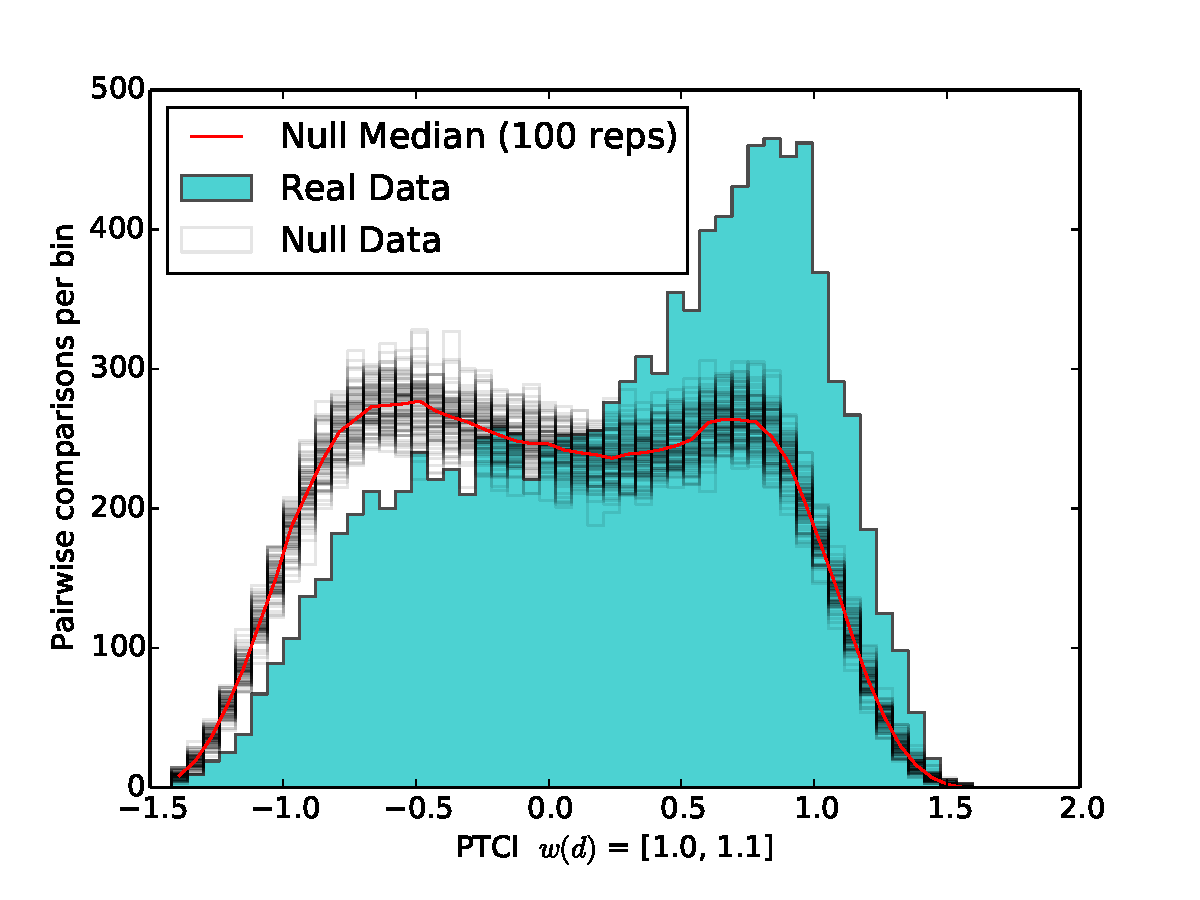
\includegraphics[width=.5\linewidth]{figures/figs/ecr_team_ptci_20130918_orthodb7/pairwise_ptci_hist.pdf}}
% 
\subcaptionbox{\label{fig:ecr-pair-ptci-hists-rcum-hist}}
{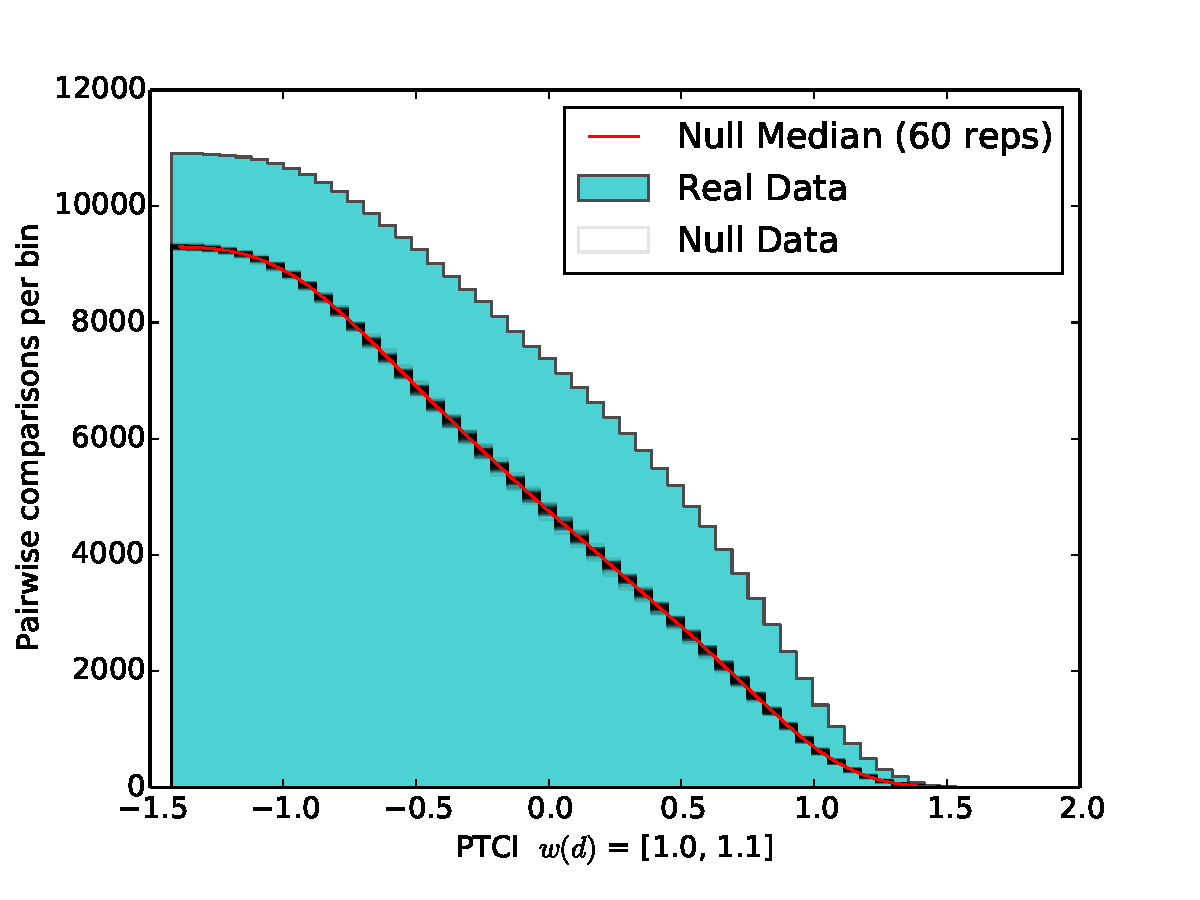
\includegraphics[width=.5\linewidth]{figures/figs/ecr_team_ptci_20130918_orthodb7/pairwise_ptci_cum_hist.pdf}}
% 
\subcaptionbox{\label{fig:ecr-pair-ptci-hists-fdr}}
{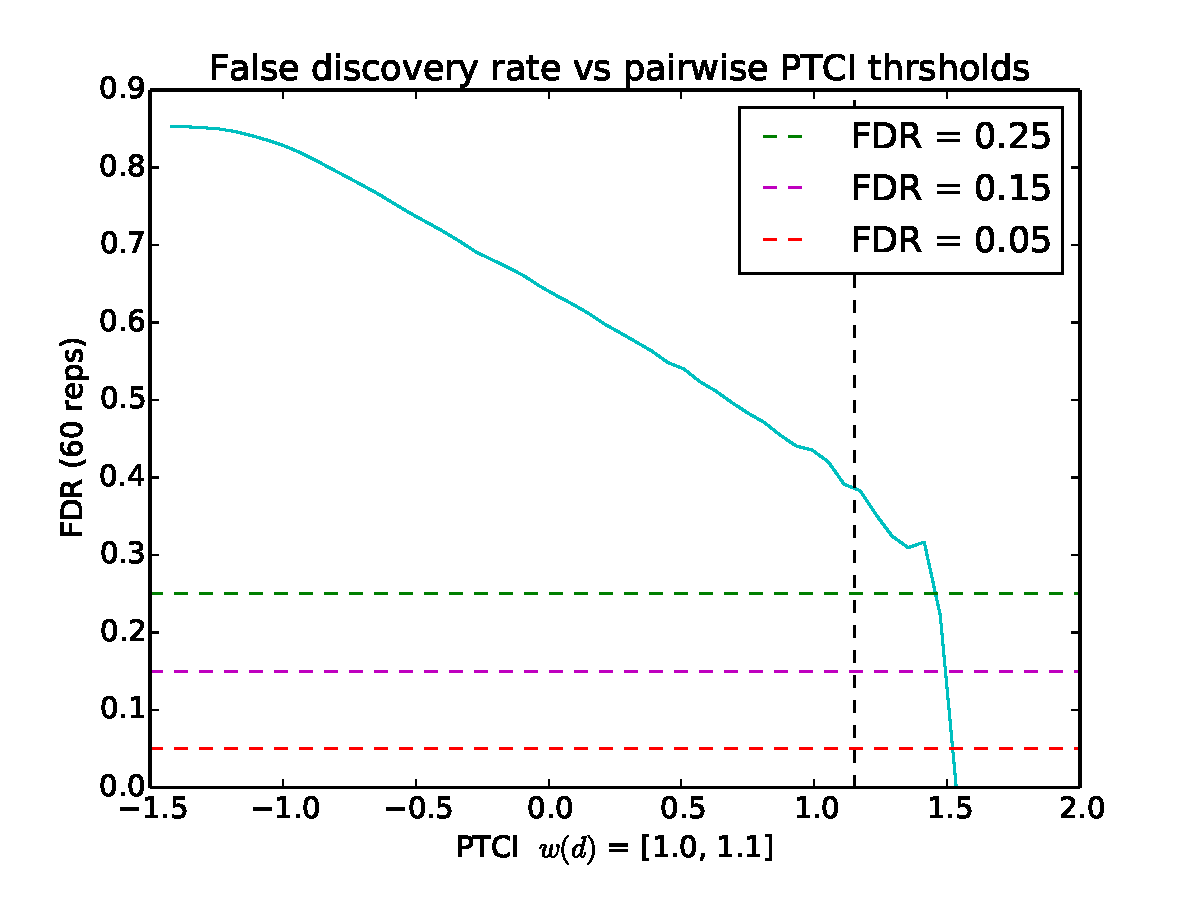
\includegraphics[width=.5\linewidth]{figures/figs/ecr_team_ptci_20130918_orthodb7/pairwise_ptci_fdr.pdf}}
% 
% 
\caption[Pairwise 20E-PTCI results]{\sf \textbf{Pairwise PTCI results for the \gls{20E}-\gls{TFBS} group}:\\
\textbf{(A)} Histogram of mean PTCI results vs null distributions.
\textbf{(B)} Reverse Cumulative histogram of mean PTCI results vs null distributions.
\textbf{(C)} False discover rate vs PTCI threshold.}
\label{fig:ecr-pair-ptci-hists}
\end{figure}

\begin{figure}[hp]
%
\subcaptionbox{\label{fig:ecr-mean-ptci-hists-base}}
{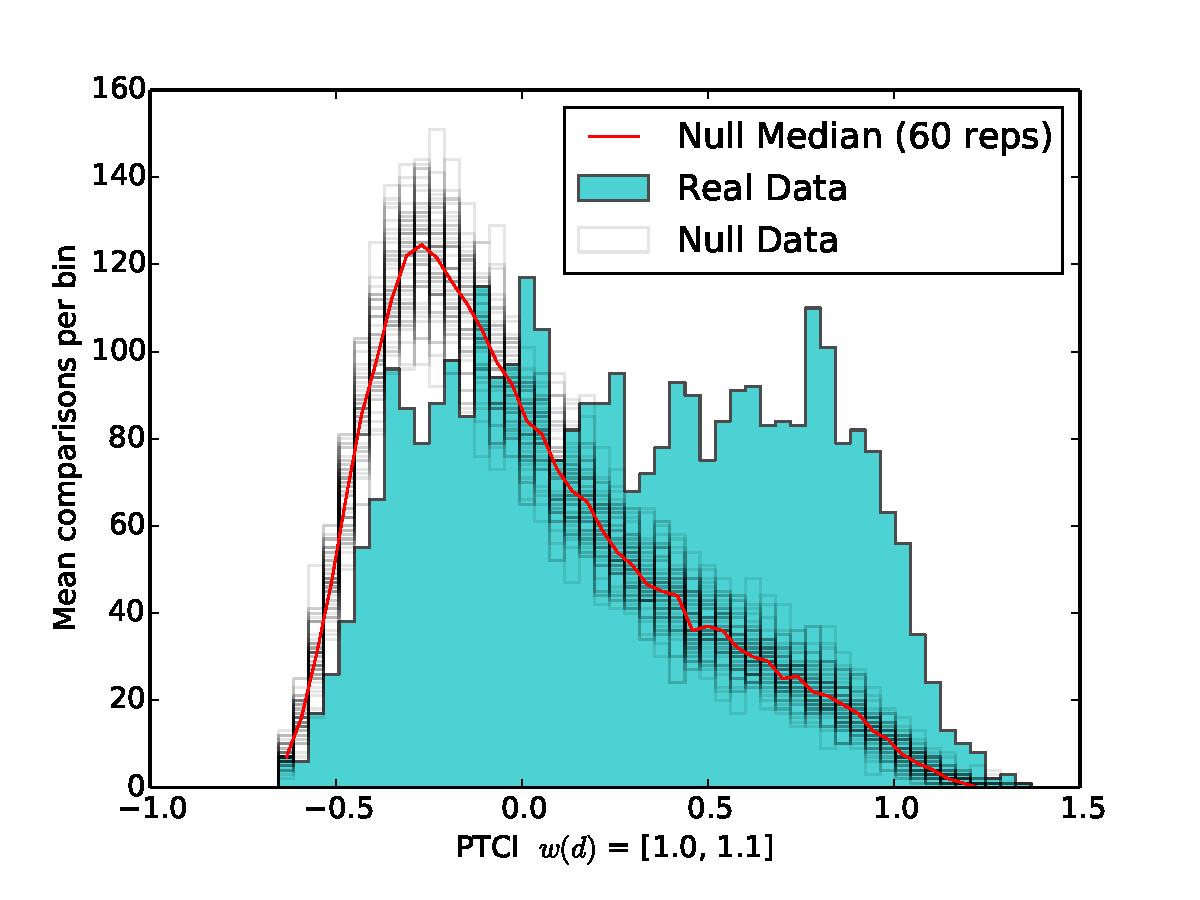
\includegraphics[width=.5\linewidth]{figures/figs/ecr_team_ptci_20130918_orthodb7/mean_ptci_hist.pdf}}
% 
\subcaptionbox{\label{fig:ecr-mean-ptci-hists-rcum-hist}}
{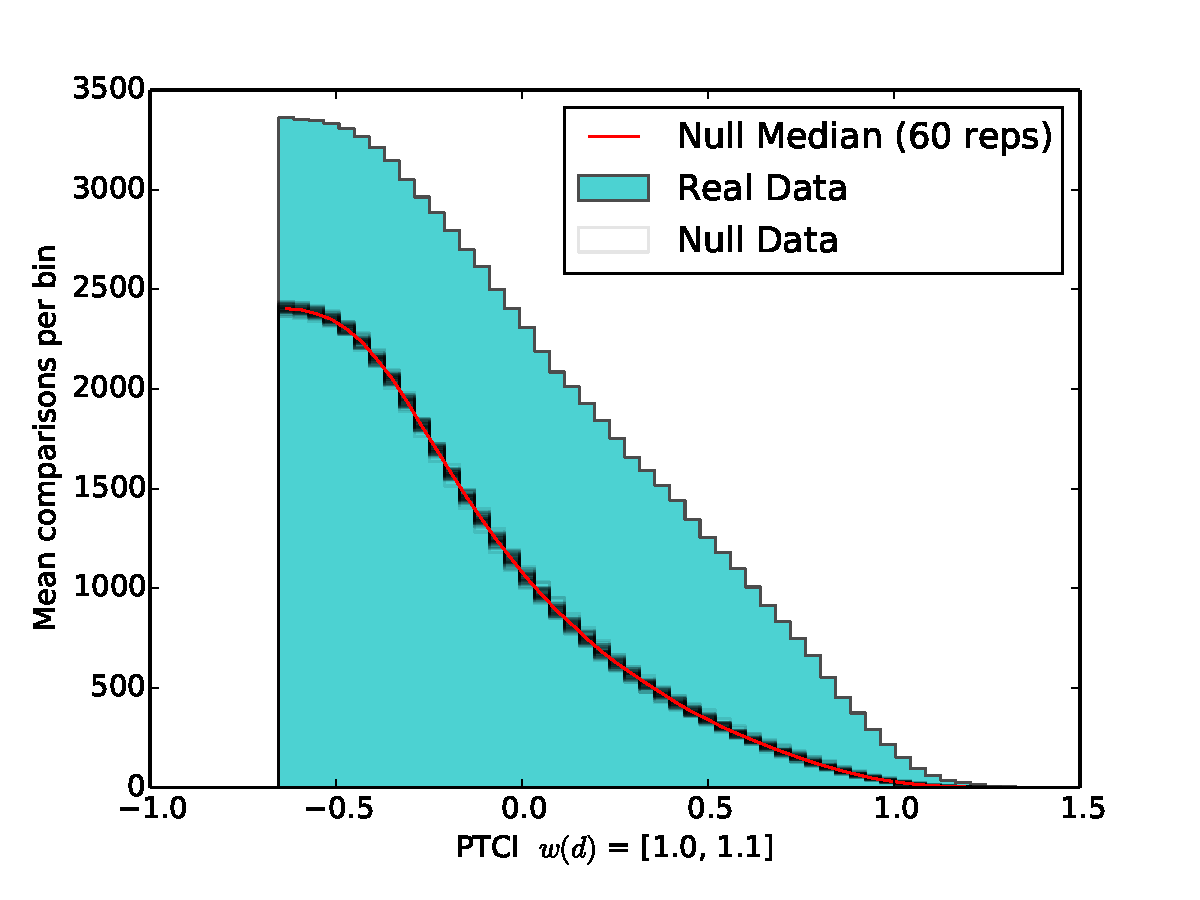
\includegraphics[width=.5\linewidth]{figures/figs/ecr_team_ptci_20130918_orthodb7/mean_ptci_cum_hist.pdf}}
% 
\subcaptionbox{\label{fig:ecr-mean-ptci-hists-fdr}}
{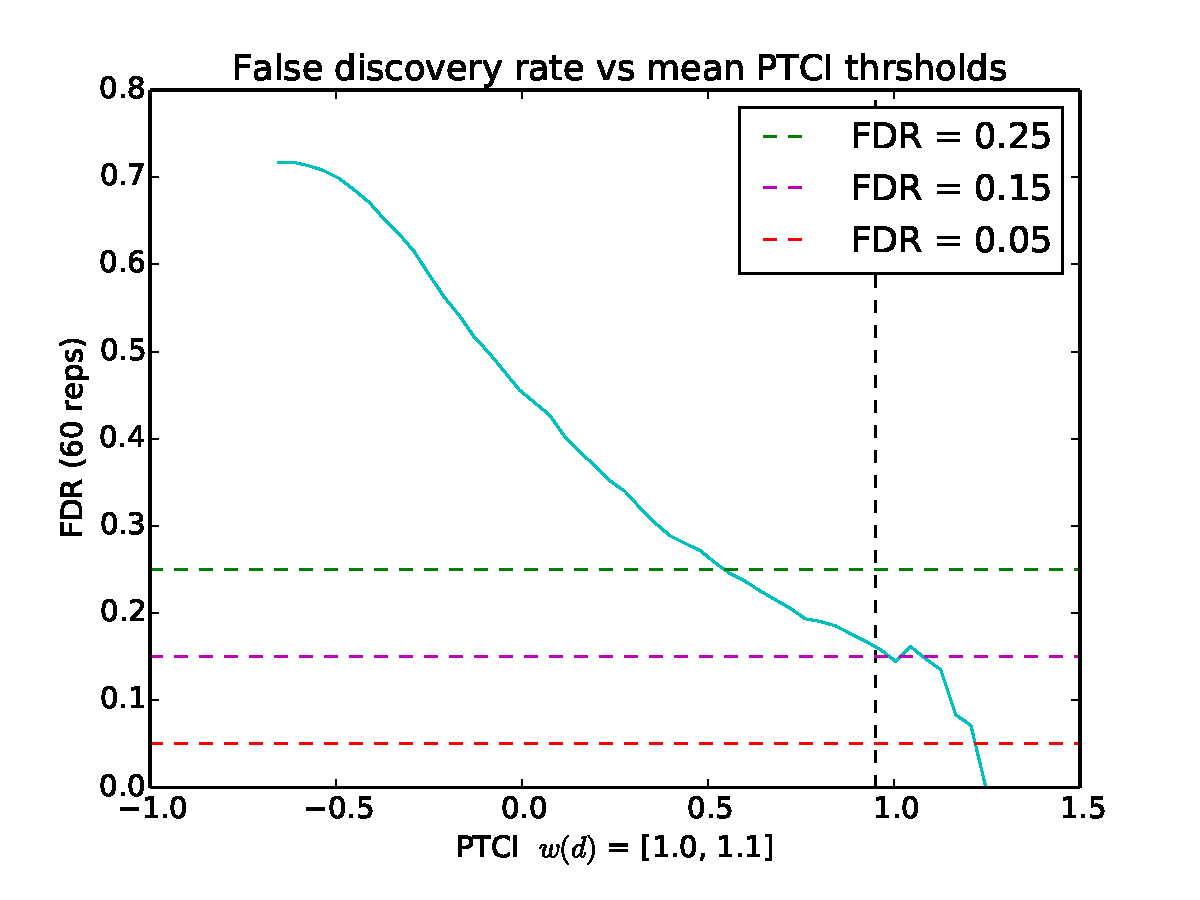
\includegraphics[width=.5\linewidth]{figures/figs/ecr_team_ptci_20130918_orthodb7/mean_ptci_fdr.pdf}}
% 
% 
\caption[Mean 20E-PTCI results]{\sf \textbf{Mean PTCI results for the \gls{20E}-\gls{TFBS} group}:\\
\textbf{(A)} Histogram of mean PTCI results vs null distributions.
\textbf{(B)} Reverse Cumulative histogram of mean PTCI results vs null distributions.
\textbf{(C)} False discovery rate vs PTCI threshold.}
\label{fig:ecr-mean-ptci-hists}
\end{figure}

\begin{figure}[hp]
%
\subcaptionbox{\label{fig:insect-pair-ptci-hists-base}}
{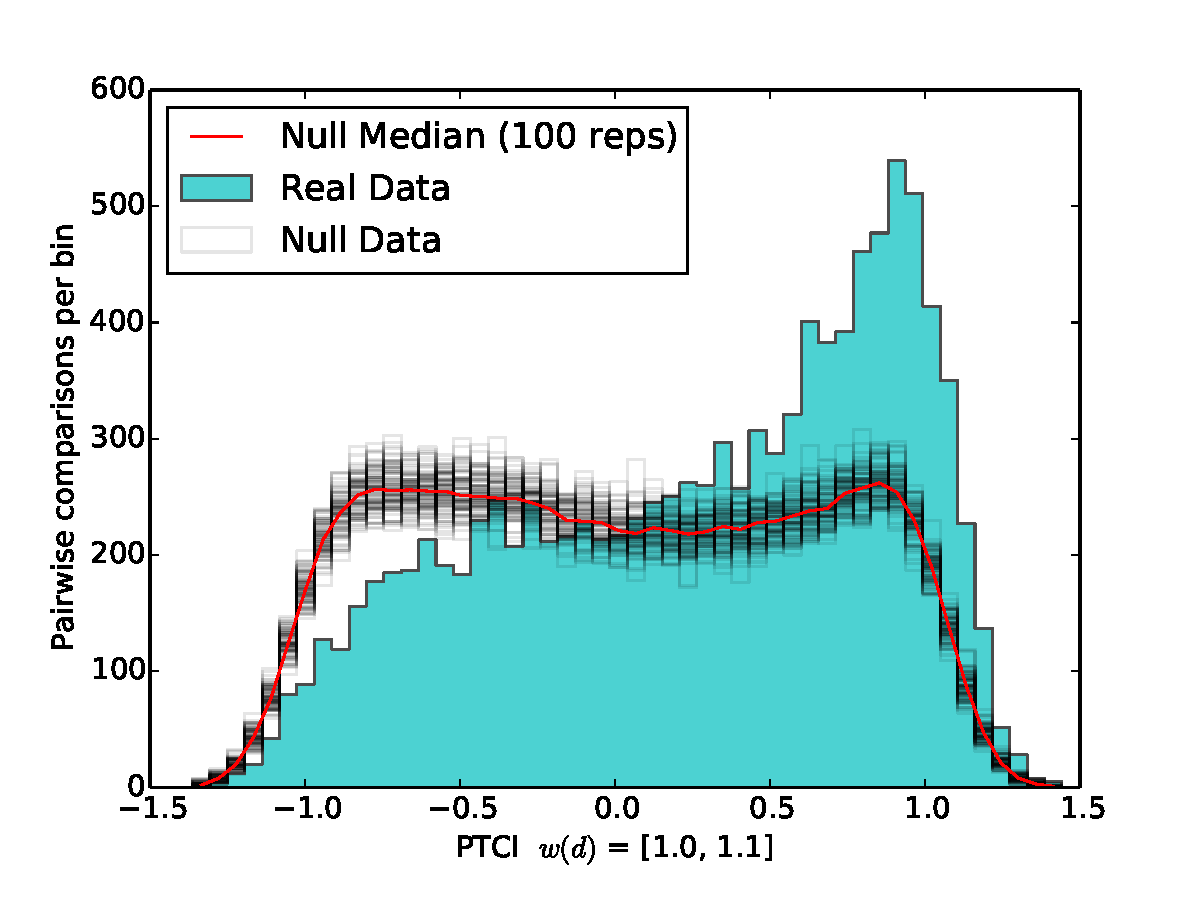
\includegraphics[width=.5\linewidth]{figures/figs/jaspar_insect_ptci_20130918_orthodb7/pairwise_ptci_hist.pdf}}
% 
\subcaptionbox{\label{fig:insect-pair-ptci-hists-rcum-hist}}
{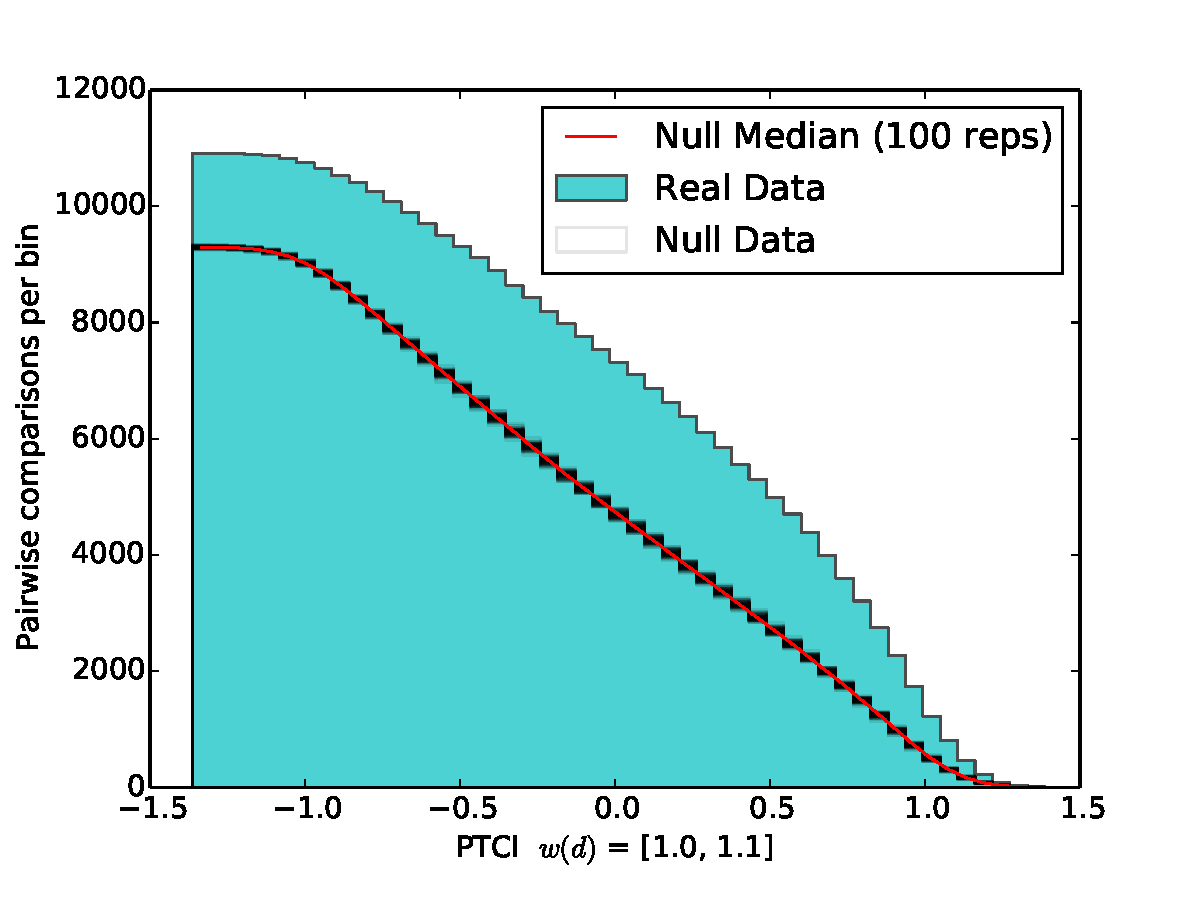
\includegraphics[width=.5\linewidth]{figures/figs/jaspar_insect_ptci_20130918_orthodb7/pairwise_ptci_cum_hist.pdf}}
% 
\subcaptionbox{\label{fig:insect-pair-ptci-hists-fdr}}
{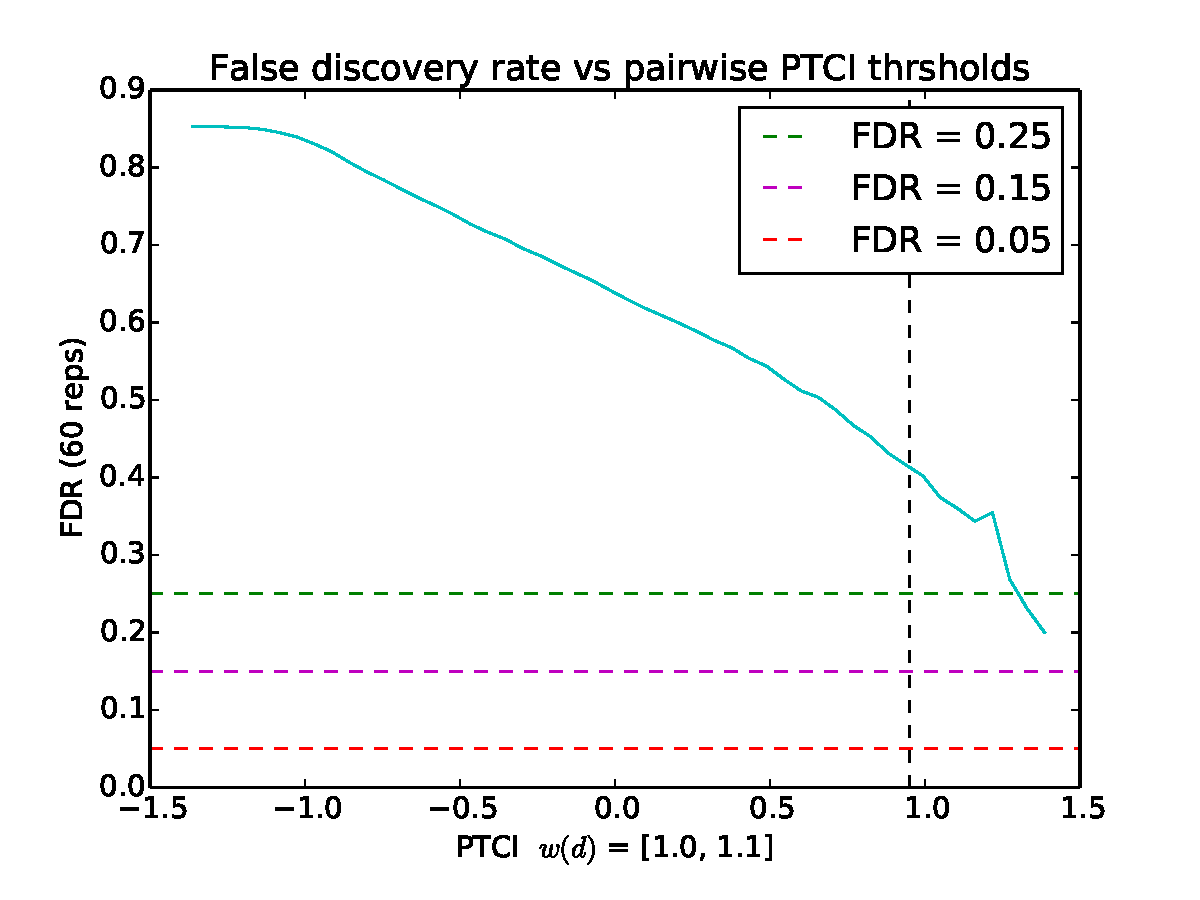
\includegraphics[width=.5\linewidth]{figures/figs/jaspar_insect_ptci_20130918_orthodb7/pairwise_ptci_fdr.pdf}}
% 
% 
\caption[Pairwise insect-PTCI results]{\sf \textbf{Pairwise PTCI results for the insect-\gls{TFBS} group}:\\
\textbf{(A)} Histogram of mean PTCI results vs null distributions.
\textbf{(B)} Reverse Cumulative histogram of mean PTCI results vs null distributions.
\textbf{(C)} False discover rate vs PTCI threshold.}
\label{fig:insect-pair-ptci-hists}
\end{figure}

\begin{figure}[hp]
% /home/gus/Dropbox/repos/git/uci-thesis-latex/figures/figs/jaspar_insect_ptci_20130918_orthodb7/mean_ptci_cum_hist.pdf
\subcaptionbox{\label{fig:insect-mean-ptci-hists-base}}
{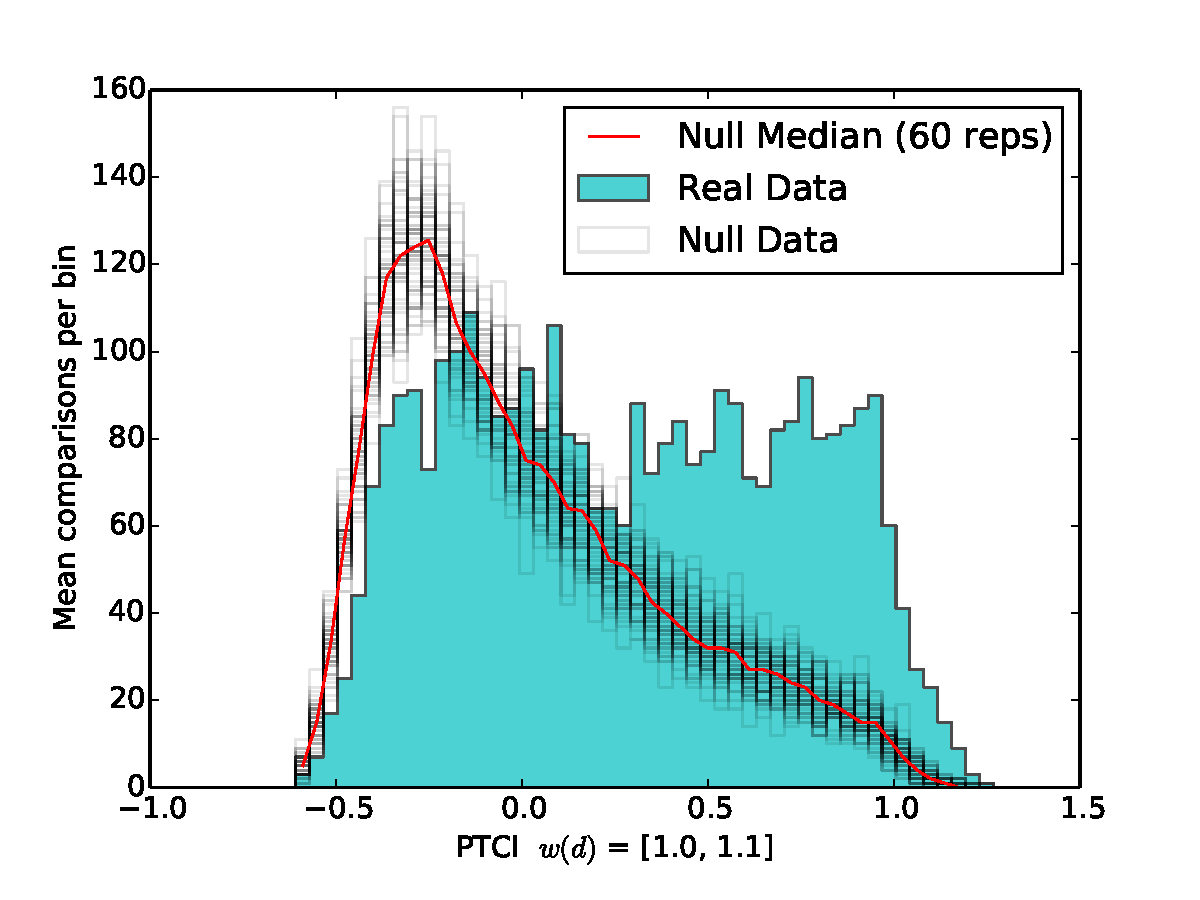
\includegraphics[width=.5\linewidth]{figures/figs/jaspar_insect_ptci_20130918_orthodb7/mean_ptci_hist.pdf}}
% 
\subcaptionbox{\label{fig:insect-mean-ptci-hists-rcum-hist}}
{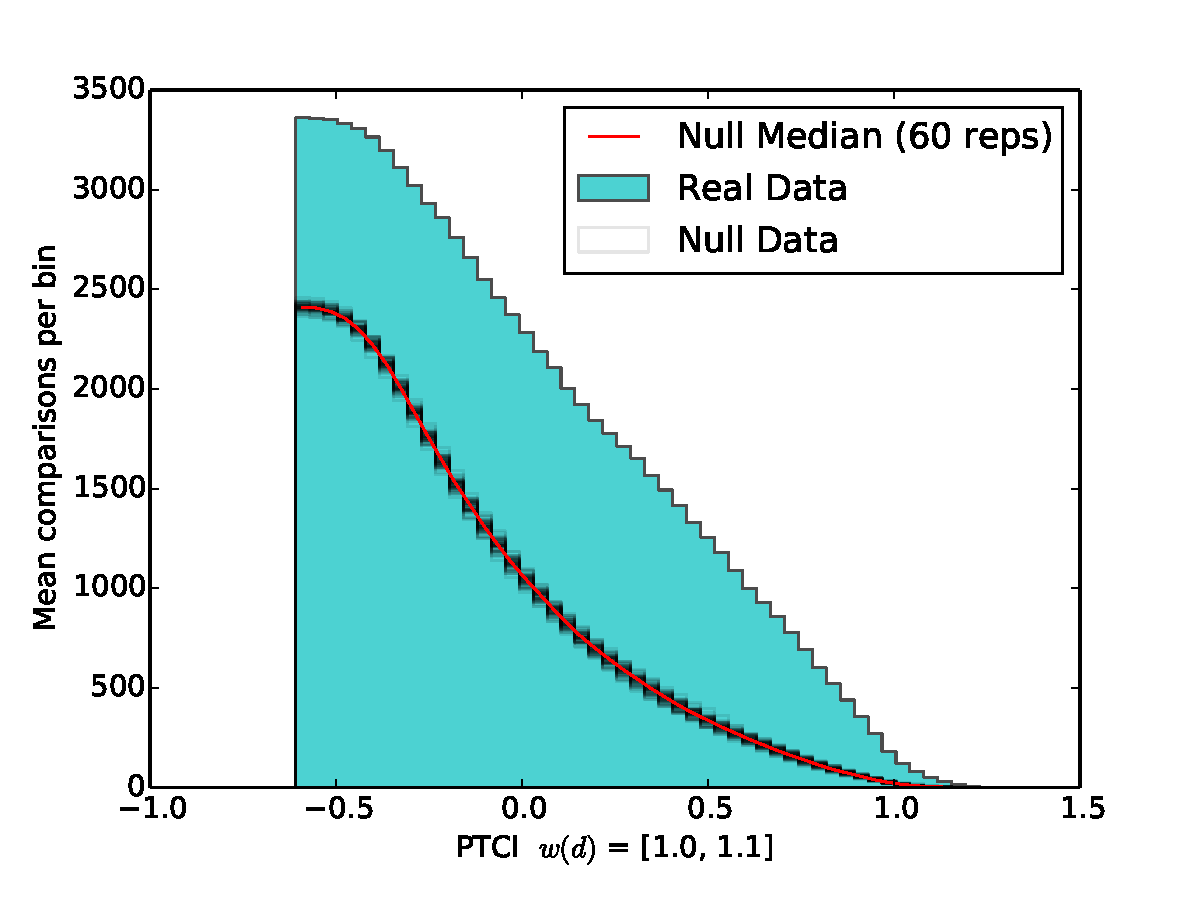
\includegraphics[width=.5\linewidth]{figures/figs/jaspar_insect_ptci_20130918_orthodb7/mean_ptci_cum_hist.pdf}}
% 
\subcaptionbox{\label{fig:insect-mean-ptci-hists-fdr}}
{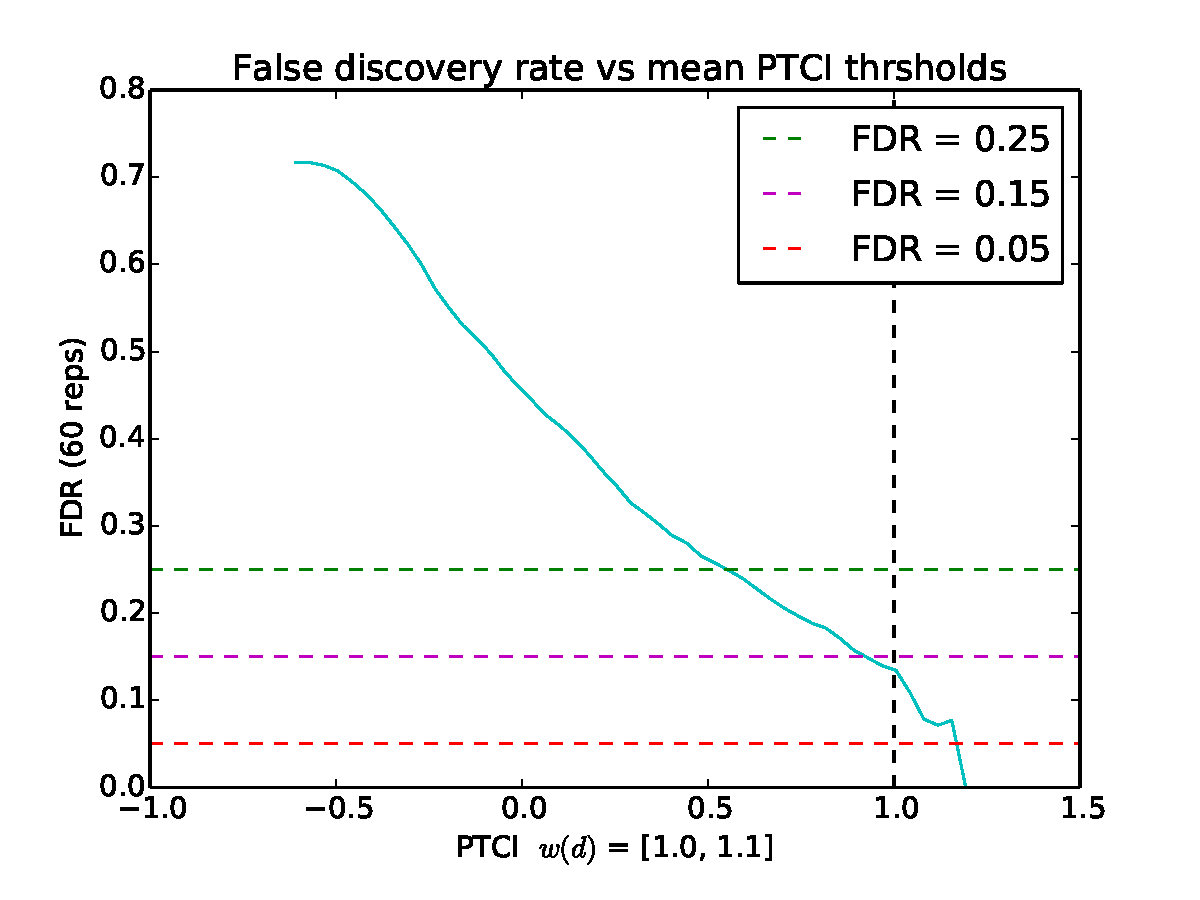
\includegraphics[width=.5\linewidth]{figures/figs/jaspar_insect_ptci_20130918_orthodb7/mean_ptci_fdr.pdf}}
% 
% 
\caption[Mean insect-PTCI results]{\sf \textbf{Mean PTCI results for the insect-\gls{TFBS} group}:\\
\textbf{(A)} Histogram of mean PTCI results vs null distributions.
\textbf{(B)} Reverse Cumulative histogram of mean PTCI results vs null distributions.
\textbf{(C)} False discover rate vs PTCI threshold.}
\label{fig:insect-mean-ptci-hists}
\end{figure}
%
\FDR\ estimation was used to determine a suitable \PTCI\ value to use as a threshold for further investigating particular 3-way 1:1 ortholog sets.
%
It was determined that in both \gls{TFBS} model data-sets a mean \PTCI\ threshold of 0.95 yielded an \FDR\ of approximately 15\% and maximized the number of genes for further classification (Figures \ref{fig:ecr-mean-ptci-hists-fdr} and \ref{fig:insect-mean-ptci-hists-fdr}).
%
This threshold produced 666 and 708 genes in the \PTCIi\ and \PTCIe\ sets, respectively.
%
The union of these gene-sets was 930 genes or 310 genes from each species.
%
The intersection was 444 or an overlap of 66\% of the \PTCIi\ genes and 62.7\% of the \PTCIe\ genes.
%
The unique proportion contributed by each set are 33\% and 37.3\%, respectively.

\paragraph*{Mean vs pairwise PTCI:}
Comparing the \FDR\ values of the pairwise- and mean-\PTCI\ scores at the 0.95 threshold reveals the impact of considering information from all 3-way 1:1 orthologs simultaneously rather than species-pair by species-pair (Figures \ref{fig:ecr-pair-ptci-hists-fdr} vs \ref{fig:ecr-mean-ptci-hists-fdr} and Figures \ref{fig:insect-pair-ptci-hists-fdr} vs \ref{fig:insect-mean-ptci-hists-fdr}).
%
The quality, as judged by \FDR, is strikingly improved by including the relationships of all three species weighted by their pairwise evolutionary distance: an improvement of approximately 30 percentage points in both cases.

\section{Characterization of results stage}
These results pertain to the third stage of the approach described in Chapter \ref{chap:3} (Figure \ref{fig:approach-chart}: \textit{blue box}).

\subsection{Functional annotations (before k-means clustering)}

Functional annotations were obtained for the 930 genes using \gls{Argot2} (Section \ref{chap:3-sec:characterization-of-results}).
%
%% How many of the 930 were assigned at least one annotation >= 200? --> 760 (Aa:253 ,Ag:254 , Cq:253 )
%% How many genes got better than 2000? --> 452 (Aa: 154, Ag:153 , Cq:145 )
Of these, 760 were assigned, by \gls{Argot2}, at least one annotation with a \gls{TS} greater than or equal to 200\footnote{This is the threshold that is suggested by the developers based on their in-house benchmarking \url{http://www.medcomp.medicina.unipd.it/Argot2/help/argot\_scores.php\#ts}} (\Aa: 253, \Ag: 254, \Cq: 253).
%
452 were assigned annotations with \glspl{TS} greater than or equal to 2000 (\Aa: 154, \Ag: 153, \Cq: 145).
%
This indicates that on the whole, most of the 930 genes produced by the \gls{gFunc} process were assigned annotations of a quality at least as stringent as used by the developers of \gls{Argot2}.

%%%%%%%%%%%%%%%%%%%%%

\subsection{K-means clustering}

K-means clustering ($k=23$) was applied to the 310 genes from \Ag\ to partition the 3-way 1:1 ortholog sets based on \gls{mAP} similarity.
%
\Ag\ was selected because it shares approximately equidistant evolutionary divergence to both other species.
%
Four of the resulting clusters were chosen for further characterization (Figure \ref{fig:23-clusters}: \textit{Cluster IDs 4, 6, 16, and 22}) because they have expression patterns that may be regulated by a noted pulse of \gls{20E} that occurs around 4h \gls{PBM}\footnote{See Section \ref{chap:3-sec:clustering-of-filtered-ortholog-sets} for more information.}.
%

\begin{landscape}

    \begin{figure}[h]
    \centering
    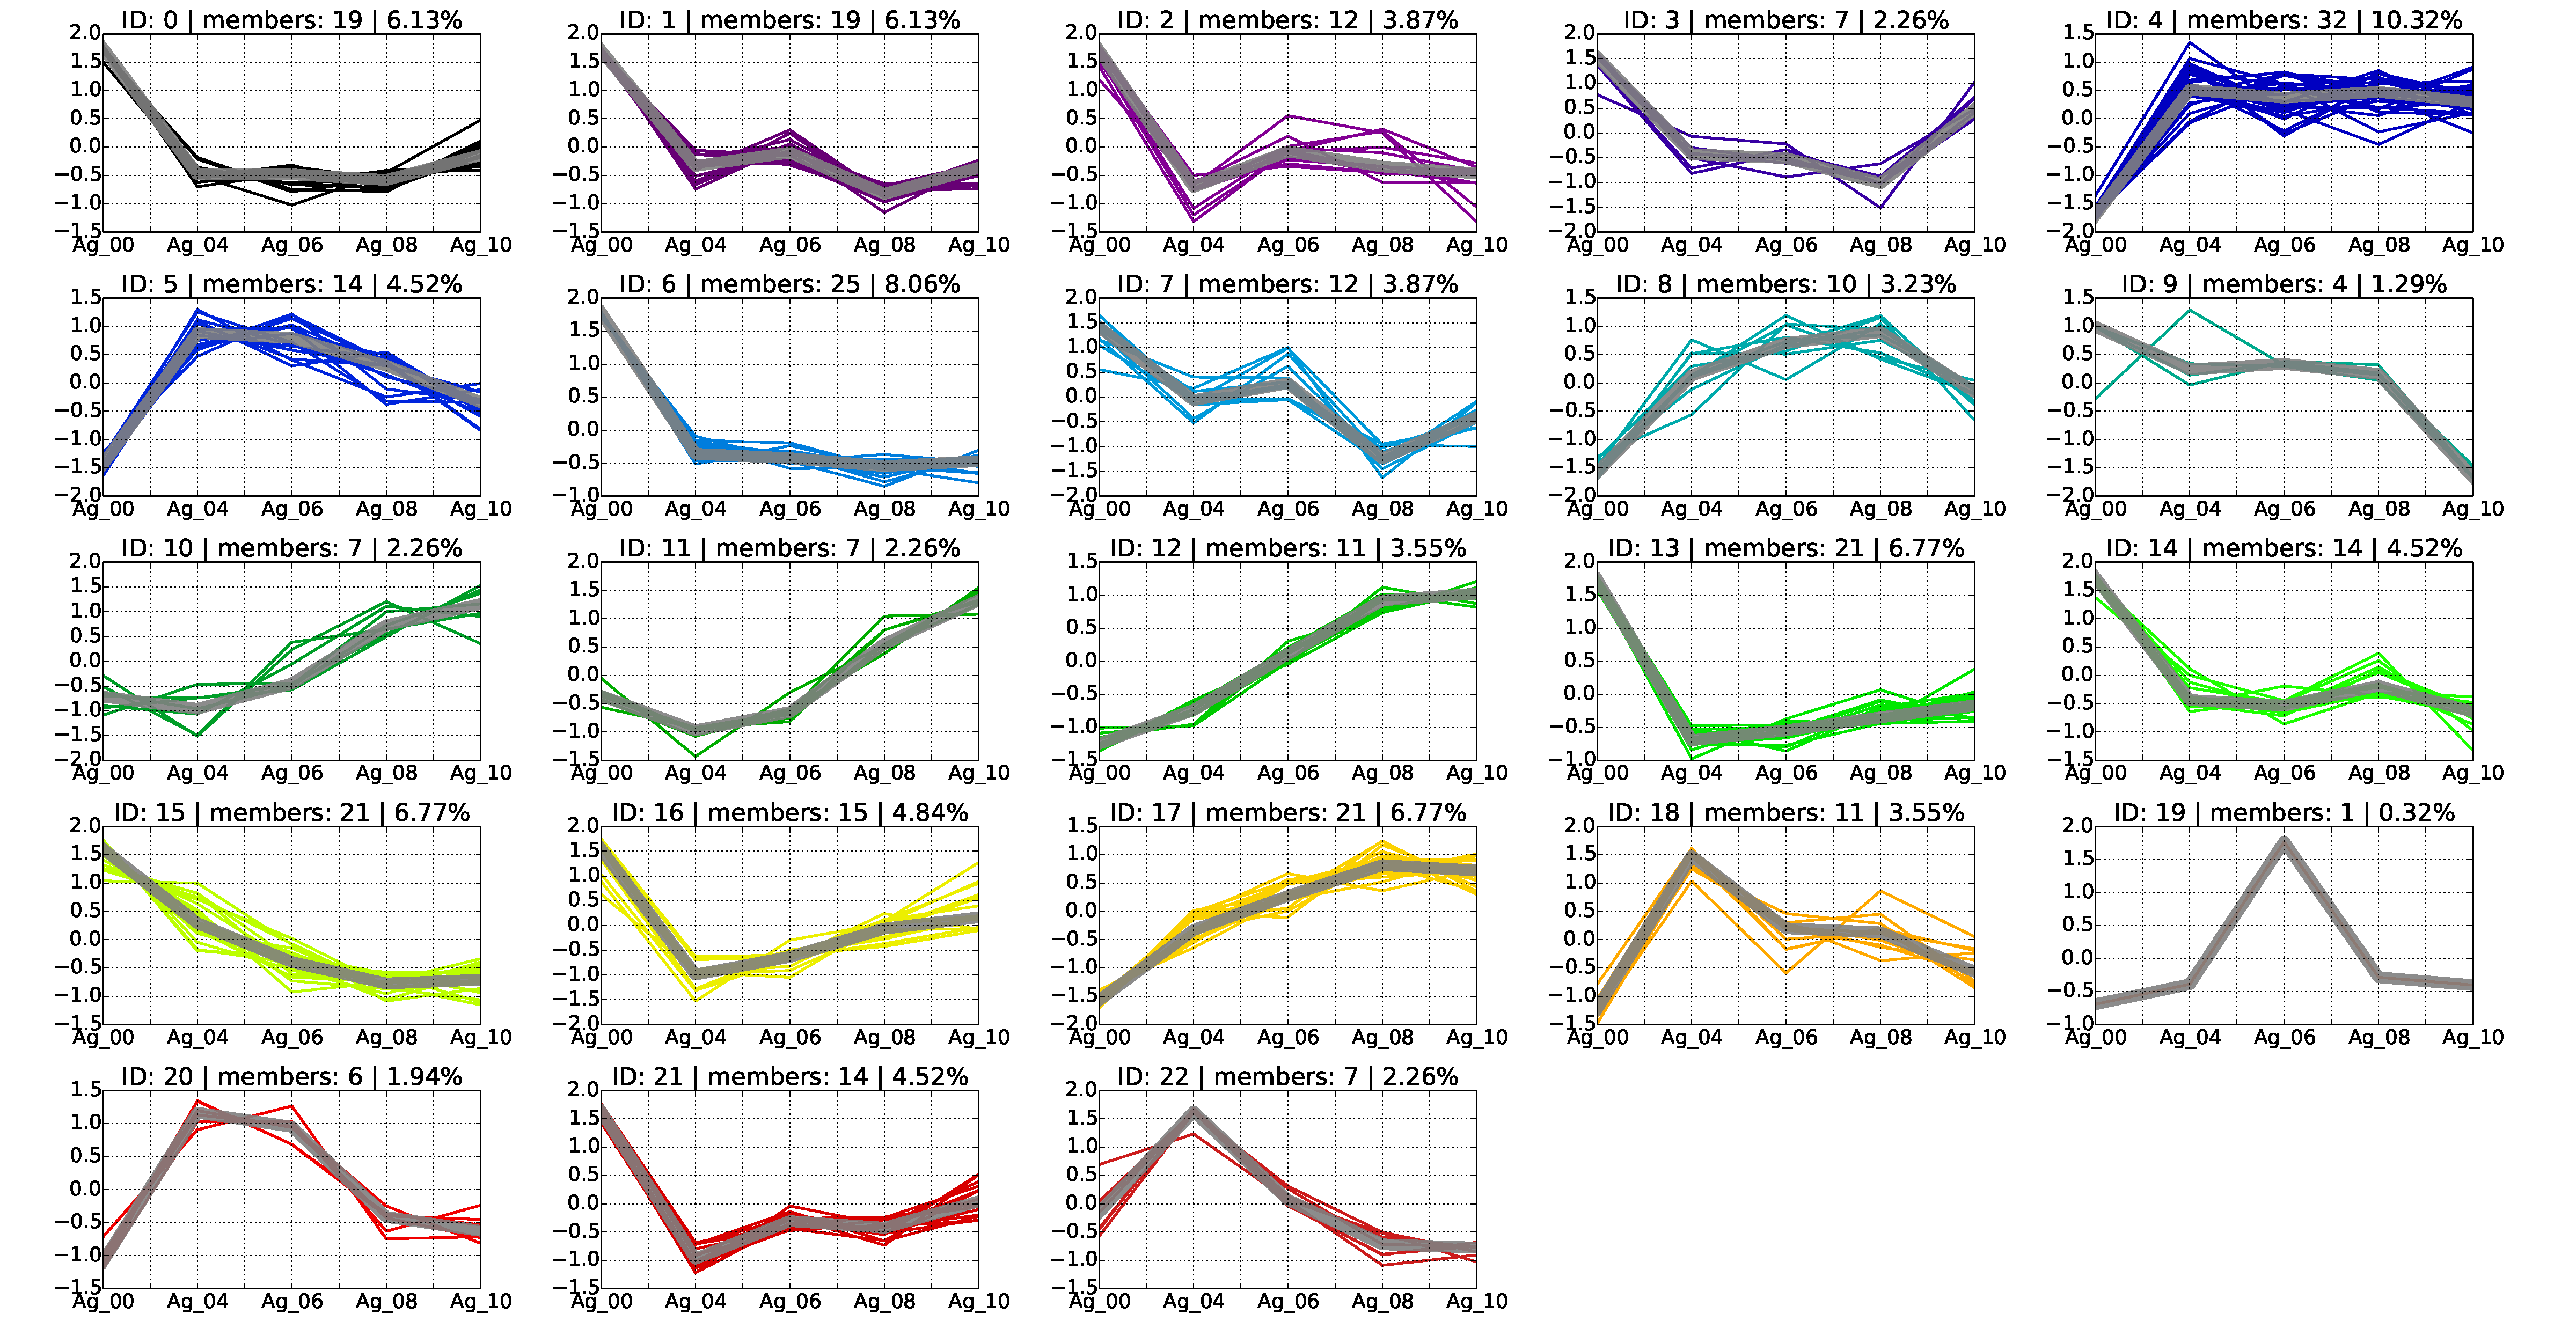
\includegraphics[width=\linewidth]{figures/figs/ecr_and_insects_ptci_20130918_orthodb7/23clusters_ptci_0_95_orthodb7.pdf}
    \caption[\Ag\ clustered abundance profiles]{\sf \textbf{\Ag\ clustered abundance profiles.} \\ 
    Clusters were generated using k-means clustering as implemented in Biopython version 1.62 \cite{Cock2009}.  Abundance profile data was log transformed after one FPKM was added to all data to remove zeros ($log_{10}(\mathrm{FPKM}+1)$).  K-means was then applied using the arithmetic mean as the center for cluster definition.  The data displayed here is the gene-wise standardization of the \textbf{raw} FPKM data such that each profile has mean = 0 and standard deviation = 1. Each median abundance profile is marked by a thick gray line. \textbf{Panel Titles} - ID: cluster identifier | members: number of genes in cluster | percentage of genes represented in all clusters. \textbf{Time Points} - \gls{NBF}, 4, 6, 8, 10 h \gls{PBM}.
}
    \label{fig:23-clusters}
    \end{figure}
    
\end{landscape}



\subsection{Highlighted clusters}

Clusters 4, 6, 16, and 22 were chosen for further characterization because they demonstrated patterns of mRNA accumulation that change sharply between \gls{NBF} and 4h \gls{PBM}.
%
Clusters 4 and 6 maintain similar \gls{FPKM} values for the remaining time points and are referred to as ``up after 4h'' (Figure \ref{fig:cluster4}) and ``down after 4h'' (Figure \ref{fig:cluster6}) respectively.
%
Clusters 16 and 22 follow the change in \gls{FPKM} at 4h \gls{PBM} by gradually trending back towards the original level of accumulation and are referred to as ``down at 4h'' (Figure \ref{fig:cluster16}) and ``up at 4h'' (Figure \ref{fig:cluster22}) respectively.
%
The interest in changes that focus on 4h \gls{PBM} stems from the description of a small but reproducible pulse of \gls{20E} that coincides with many important events which signal the switch from a \gls{JH} dominated signaling environment to one influenced by the lack of \gls{JH} and presence of \gls{20E}\footnote{See Discussion (Section \ref{chap:4-sec:discussion}) for more details.}

The cluster-specific functional annotation results included in the following sections represent the mean \gls{TS} for all occurrences of each term in the cluster-specific \gls{Argot2} results.
%
This provides an overview of which function and process gene ontology terms characterize the cluster as a whole as opposed to each individual gene.

\subsubsection{Cluster 4 (up after 4h)}

\paragraph*{General description:}

Cluster 4 is characterized by genes that have a median \gls{NBF} \gls{FPKM} of approximately 1.5 standard deviations \textit{below} their overall mean \gls{FPKM} \gls{FPKM} and median \gls{FPKM} values between 0 and 0.5 standard deviations \textit{above} their overall mean \gls{FPKM} for the remainder of the time course (Figures \ref{fig:23-clusters} and \ref{fig:cluster4}).
%
This \gls{mAP} illustrates a rapid and sustained increase in mRNA abundance putatively triggered by the bloodfeeding stimulus.
%
\begin{figure}[p]
% 
\subcaptionbox{\label{fig:cluster4-Aa}}
{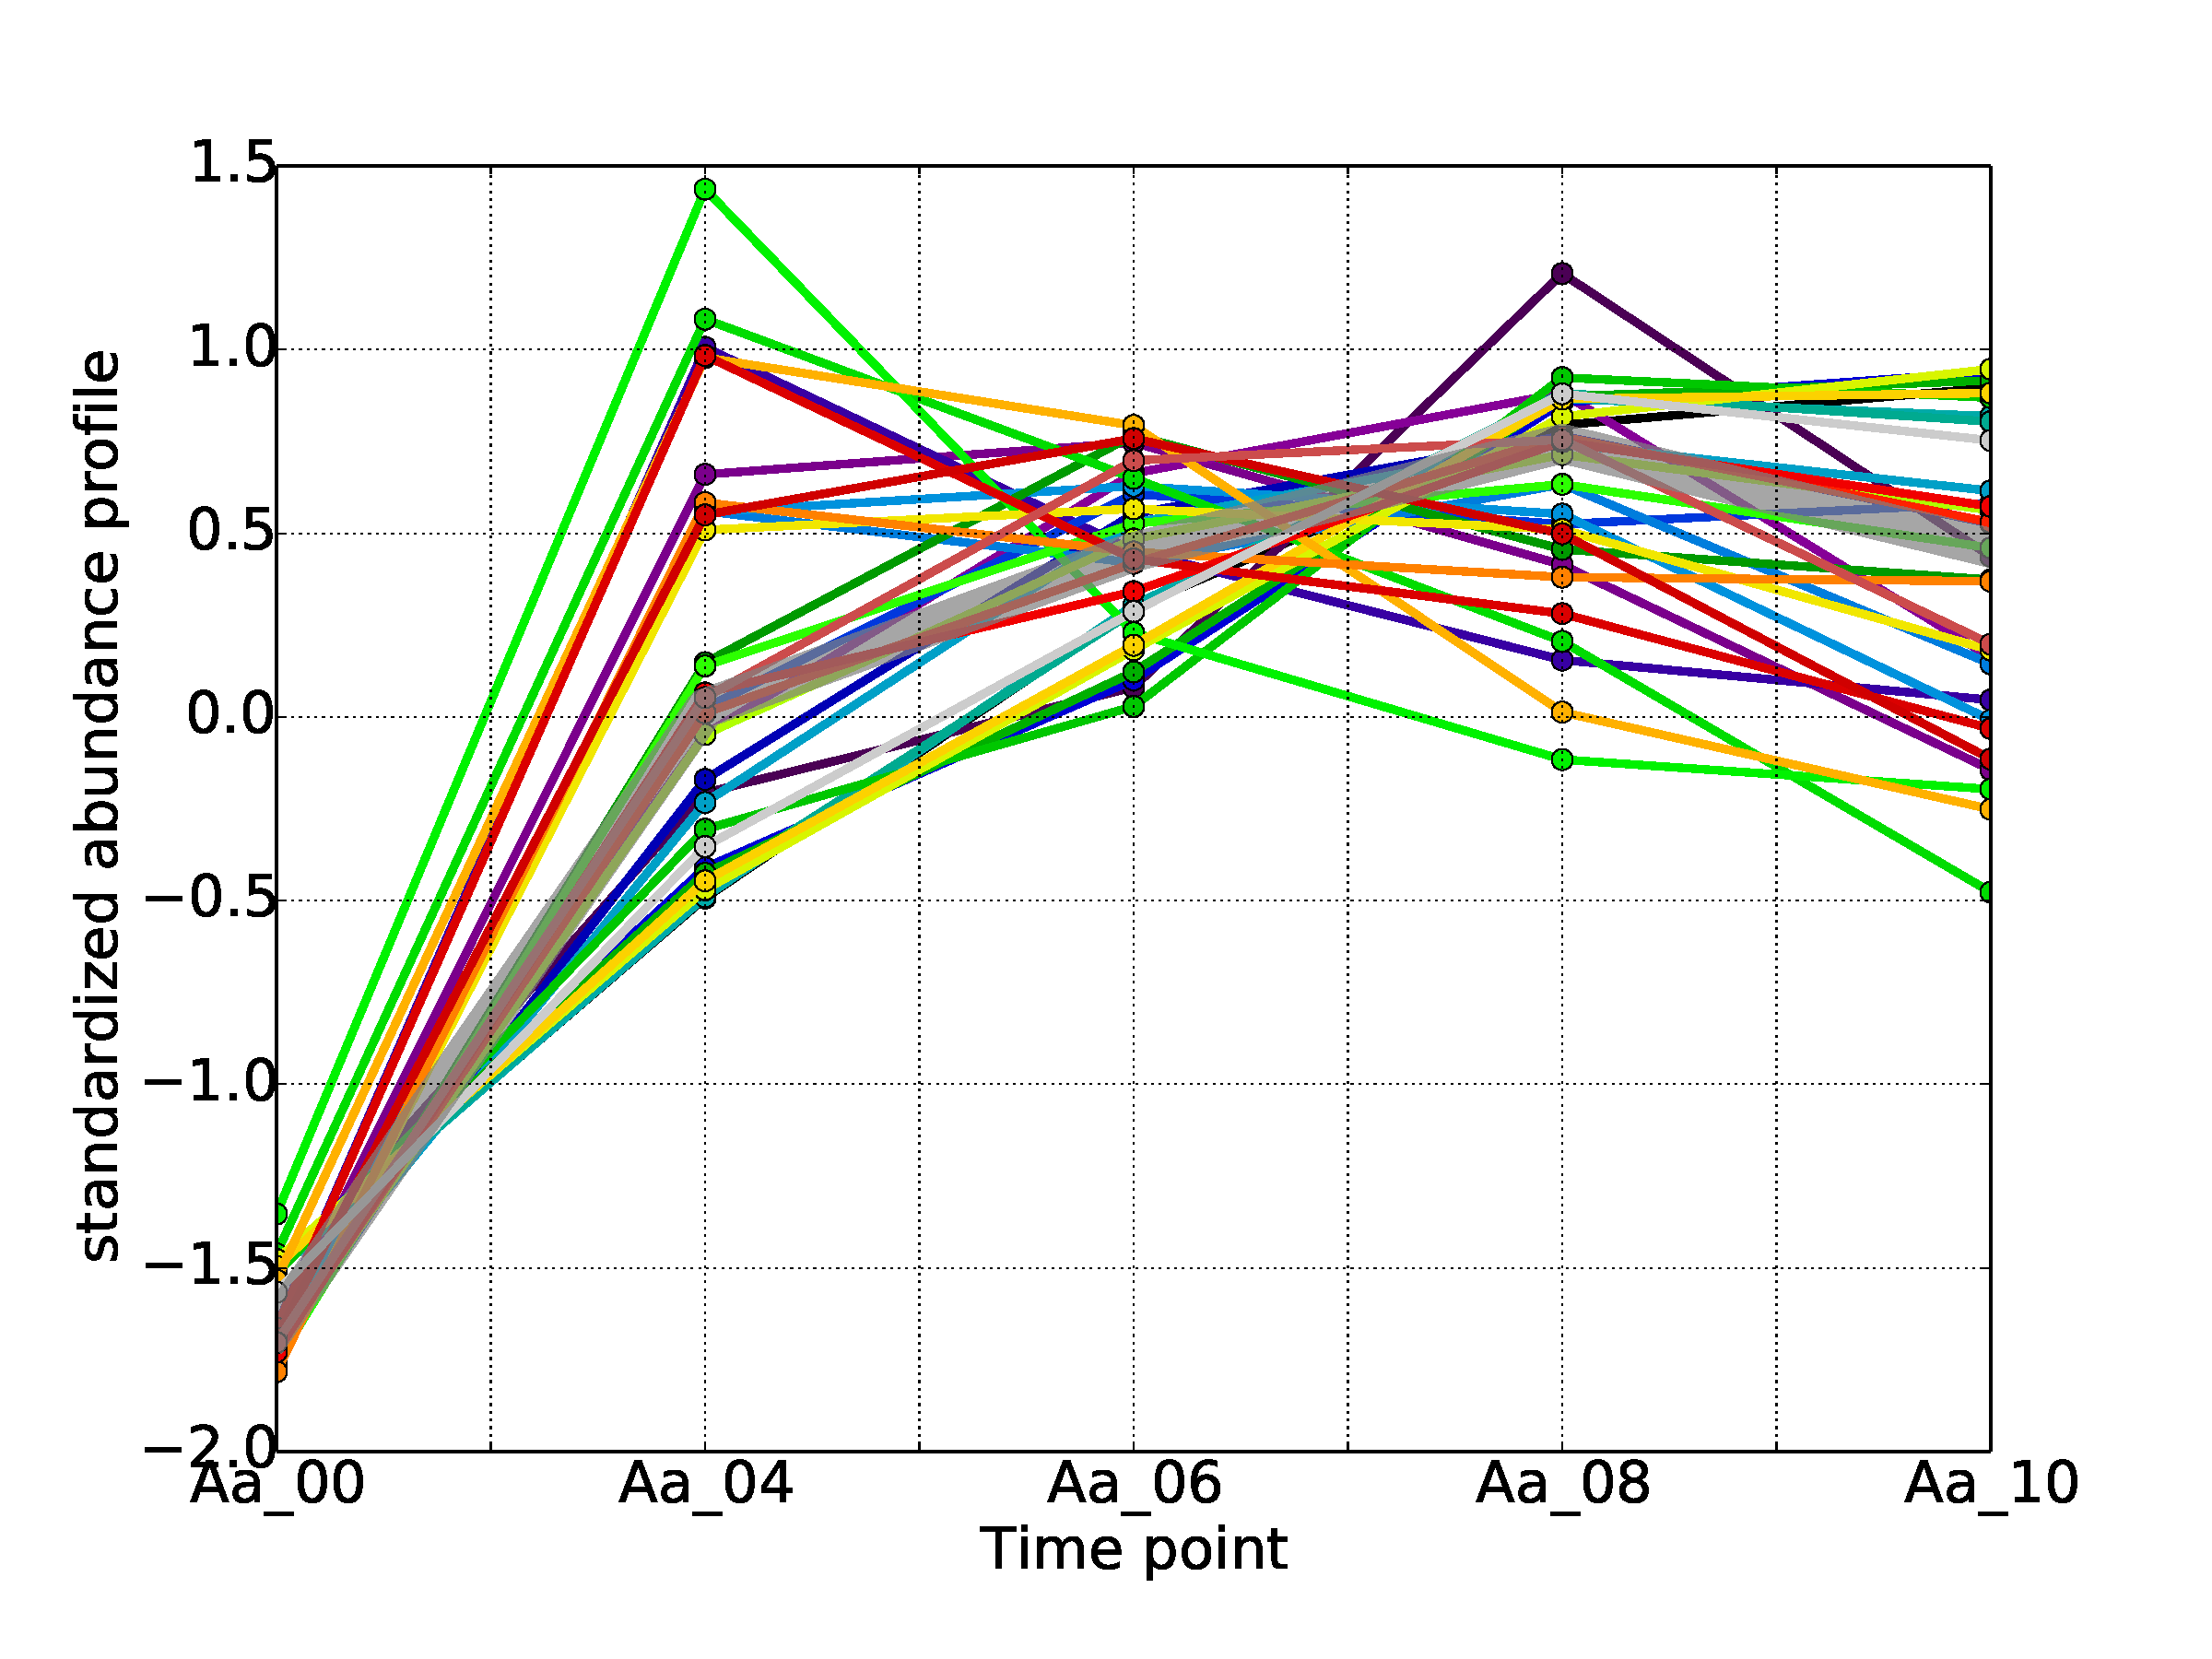
\includegraphics[width=.5\linewidth]{figures/figs/ecr_and_insects_ptci_20130918_orthodb7/upAfter4_gene_profiles_from_cummerbund/Aa_upAfter4_cls4_Ag_target_FPKMs_vb_orthos.pdf}}
%
\subcaptionbox{\label{fig:cluster4-Ag}}
{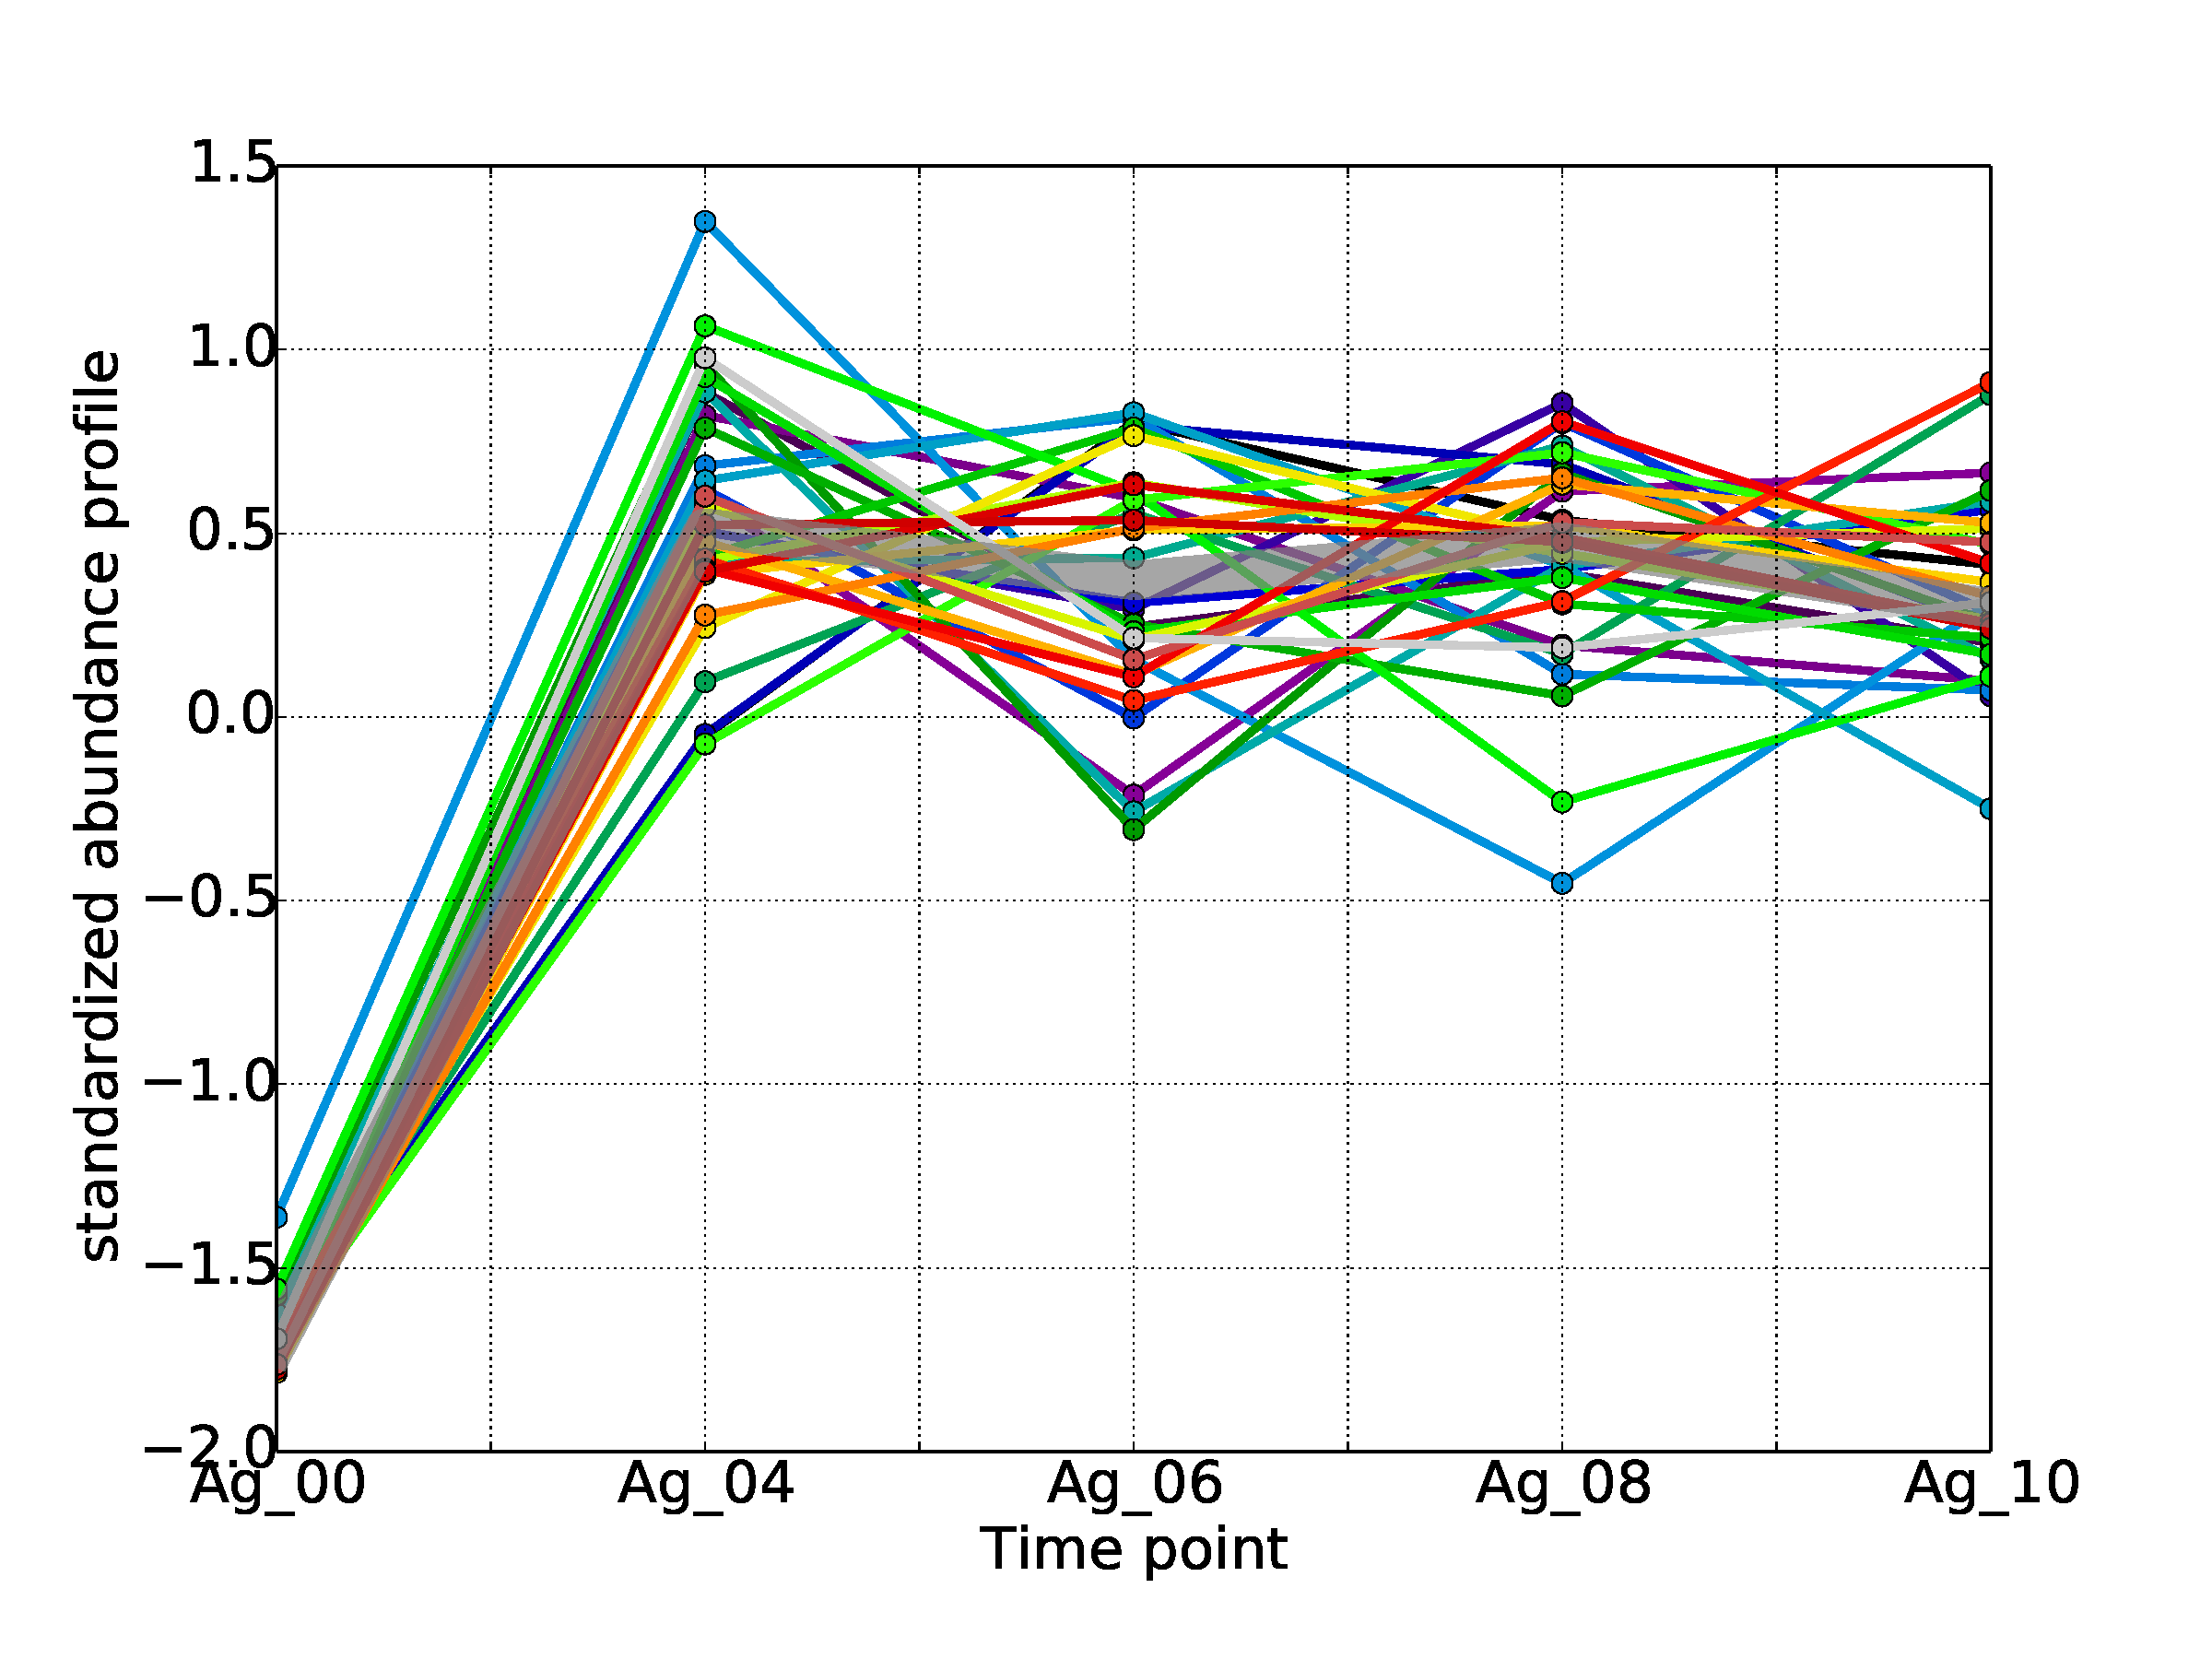
\includegraphics[width=.5\linewidth]{figures/figs/ecr_and_insects_ptci_20130918_orthodb7/upAfter4_gene_profiles_from_cummerbund/Ag_upAfter4_cls4_Ag_target_FPKMs_vb_orthos.pdf}}
%
\subcaptionbox{\label{fig:cluster4-Cq}}
{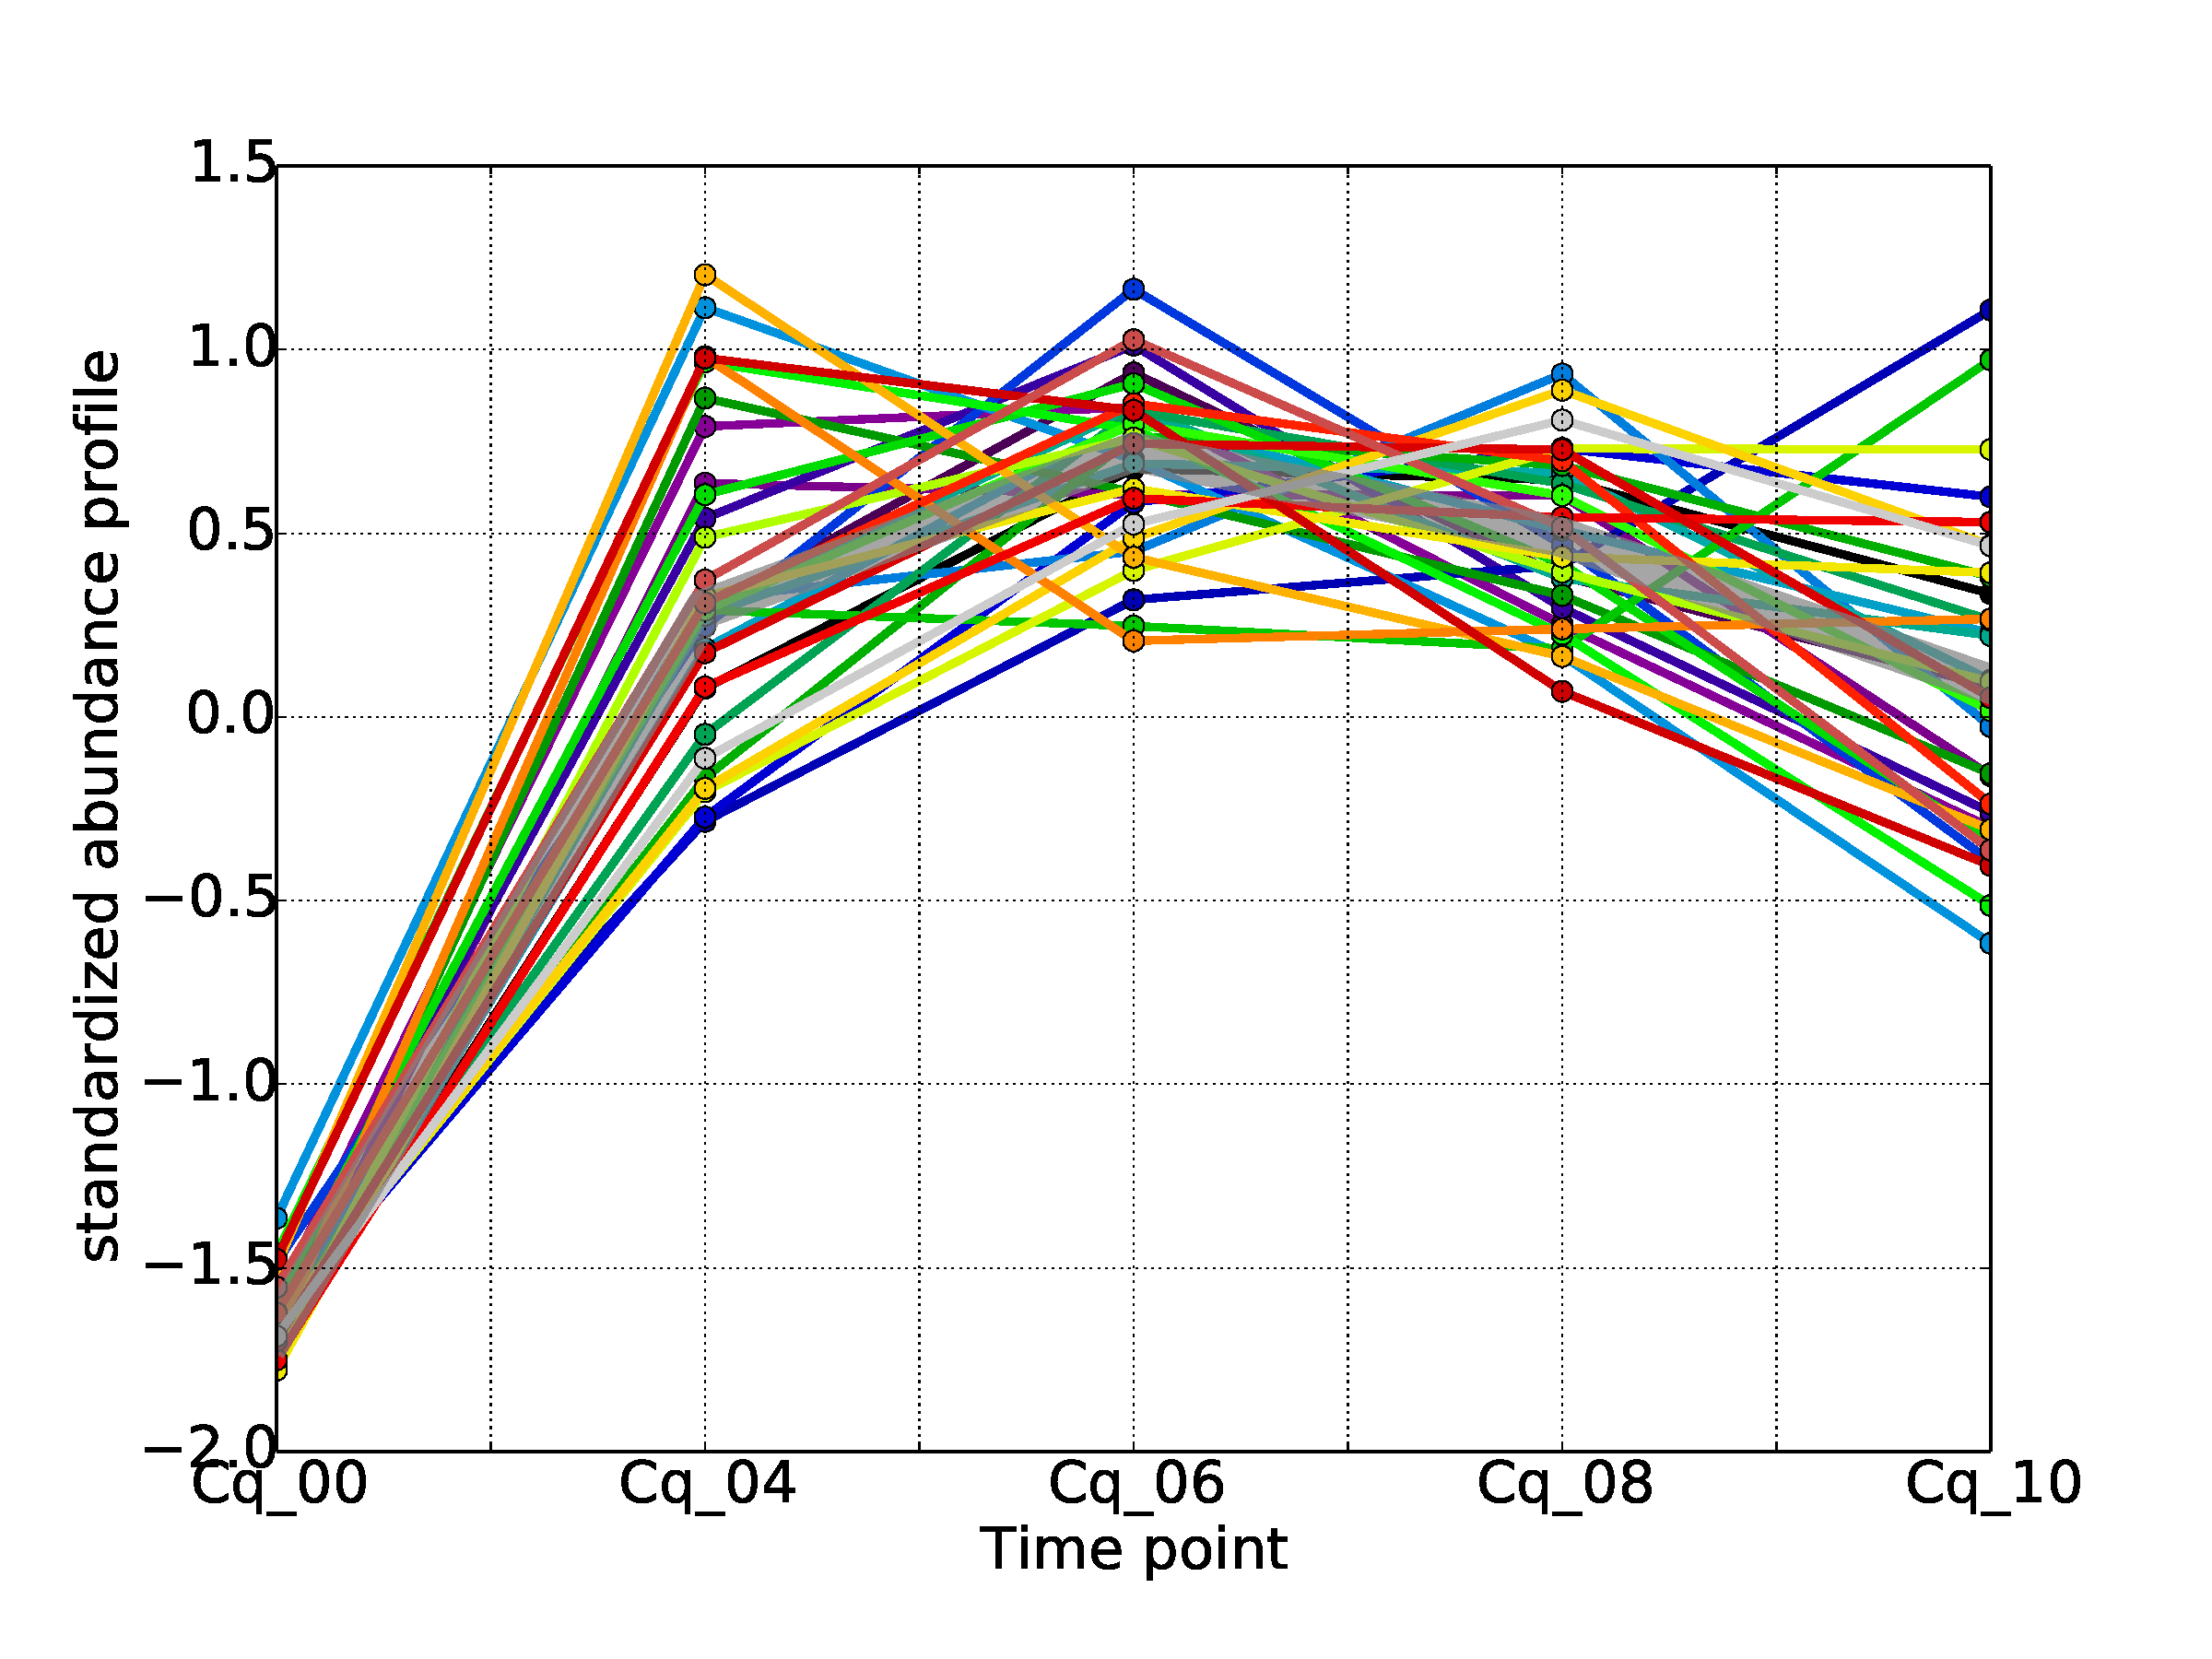
\includegraphics[width=.5\linewidth]{figures/figs/ecr_and_insects_ptci_20130918_orthodb7/upAfter4_gene_profiles_from_cummerbund/Cq_upAfter4_cls4_Ag_target_FPKMs_vb_orthos.pdf}}
% 
\caption[Orthologs of cluster 4]{\sf \textbf{Orthologs of cluster 4 (up after 4h):}\\
The same color scheme is used for each species which means that orthologs are given the same color in all three panels.
The thick, transparent gray line represents the median \gls{mAP} for the panel.
\textbf{(A)} \Aa.
\textbf{(B)} \Ag.
\textbf{(C)} \Cq.
}\label{fig:cluster4}
\end{figure}

\paragraph*{Functional annotations of cluster 4:}

% upregulation of translation/TOR
%	peptide quality control 
% active secretory pathways in both directions
% Metabolic activities

% Heme management
% midgut repair

The three main themes present in the \gls{Argot2} functional annotation terms for this cluster can be described as translation, secretory processes, and peptide metabolic activities.
%
Other supported activities include heme management and midgut repair (Tables \ref{tab:cls4-process} and \ref{tab:cls4-function}).
% Booktabs require to add \usepackage{booktabs} to your document preamble
\begin{table}[hp]
\begin{center} \sf
\begin{tabular}{p{.7\textwidth}r}
\toprule
\textbf{Name}                                                 & \textbf{Total Score (mean)} \\ \midrule
SRP-dependent cotranslational protein targeting to membrane   & 13254.87                    \\ % secretion / nutrient pathway
Golgi organization                                            & 7289.78                     \\ % secretion / nutrient pathway
glutamine biosynthetic process                                & 7056.26                     \\
bone development                                              & 6844.92                     \\ % #EXPLAIN #LOOKUP << LOOK HERE: http://pfam.sanger.ac.uk/family/PF09742 --> Functionally this protein might be involved in vesicle secretion or be an inter-cellular signalling protein or be a novel insulin receptor.[PMID 14504222] >>
ER to Golgi vesicle-mediated transport                        & 5914.05                     \\
heme biosynthetic process                                     & 5069.12                     \\ % bloodmeal
regulation of translational initiation                        & 4594.46                     \\ % translation/ TOR?
formation of translation preinitiation complex                & 4524.89                     \\ % translation/ TOR?
translational initiation                                      & 4288.82                     \\
translation                                                   & 3777.61                     \\
% positive regulation of GTPase activity                        & 3543.72                     \\
proteasome assembly                                           & 3326.44                     \\ % upregulated translation
porphyrin-containing compound biosynthetic process            & 3077.12                     \\ % #EXPLAIN #LOOKUP {{ferrochetalase}}
proton transport                                              & 2772.26                     \\ % digestion? endocytosis?
% ATP catabolic process                                         & 2642.02                     \\ % consumption of ATP / energy for proton transport?
proteolysis                                                   & 2453.58                     \\ % digestion
regulation of autophagy                                       & 2294.64                     \\ % change from starvation to nutrient excess
retrograde vesicle-mediated transport, Golgi to ER            & 2202.55                     \\
L-lysine catabolic process to acetyl-CoA via saccharopine     & 2148.61                     \\
vesicle fusion with Golgi apparatus                           & 2141.47                     \\
proteolysis involved in cellular protein catabolic process    & 1972.16                     \\
ubiquitin-dependent protein catabolic process                 & 1963.42                     \\
nitrogen compound metabolic process                           & 1885.16                     \\ % #EXPLAIN
ATP hydrolysis coupled proton transport                       & 1860.32                     \\ 
cell-cell adhesion                                            & 1774.89                     \\ % Midgut repair?
small GTPase mediated signal transduction                     & 1693.93                     \\
% response to drug                                              & 1507.48                     \\
% Golgi vesicle transport                                       & 1410.43                     \\
% intracellular protein transport                               & 1382.58                     \\
oligopeptide transport                                        & 1243.85                     \\
% cellular membrane fusion                                      & 1216.84                     \\
protein ubiquitination                                        & 1073.12                     \\
transmembrane transport                                       & 1025.68                     \\
vesicle-mediated transport                                    & 930.96                      \\
% protein transport                                             & 905.51                      \\
% mitotic prophase                                              & 897.77                      \\
% peptide transport                                             & 721.42                      \\
% transport                                                     & 657.84                      \\
% oocyte growth                                                 & 543.51                      \\ % endoplasmic reticulum organization and vesical trafficing (this gene known important in nurse cell folicle relationship) {{Protein jagunal}}
ion transport                                                 & 480.36                      \\
glycine biosynthetic process, by transamination of glyoxylate & 464.76                      \\
autophagy                                                     & 447.12                      \\
L-lysine catabolic process                                    & 417.84                      \\
lysine catabolic process                                      & 414.33                      \\
% oogenesis                                                     & 406.52                      \\
L-cysteine catabolic process                                  & 378.10                      \\
exocytosis                                                    & 294.15                      \\ % digestive secretion ? {{Protein jagunal}} endoplasmic reticulum organization and vesical trafficing
% cell adhesion                                                 & 286.17                      \\
cell differentiation                                          & 279.02                      \\ % midgut repair ?
detoxification of cadmium ion                                 & 262.31                      \\
% multicellular organismal development                          & 253.99                      \\
small molecule metabolic process                              & 253.25                      \\
metabolic process                                             & 235.09                      \\
cellular nitrogen compound metabolic process                  & 234.76                      \\
lysine biosynthetic process                                   & 207.74                      \\
cellular amino acid biosynthetic process                      & 200.81                      \\ \bottomrule                                                           
\end{tabular}
\end{center}

\caption[Cluster 4 top process GO terms]{\sf \textbf{Cluster 4 top process GO terms}}
\label{tab:cls4-process}
\end{table}
% Booktabs require to add \usepackage{booktabs} to your document preamble
\begin{table}[hp]
\begin{center} \sf
\begin{tabular}{p{.7\textwidth}r}
\toprule
\textbf{Name}                                                                                  & \textbf{Total Score (mean)} \\ \midrule
translation initiation factor activity                                                         & 18796.17                    \\ % translation/ TOR?
protein transporter activity                                                                   & 13663.10                    \\
signal recognition particle binding                                                            & 9157.88                     \\
endoplasmic reticulum signal peptide binding                                                   & 7943.20                     \\ % secretion 
Rab GDP-dissociation inhibitor activity                                                        & 7361.38                     \\
hydrolase activity, acting on acid anhydrides, catalyzing transmembrane movement of substances & 6647.91                     \\
hydrogen ion transmembrane transporter activity                                                & 6278.87                     \\
ferrochelatase activity                                                                        & 4990.12                     \\
GTP binding                                                                                    & 4006.06                     \\
%enzyme binding                                                                                 & 3697.54                     \\
saccharopine dehydrogenase (NAD+, L-glutamate-forming) activity                                & 3453.61                     \\
zinc ion binding                                                                               & 3215.15                     \\
glutamate-ammonia ligase activity                                                              & 2901.02                     \\
RNA binding                                                                                    & 2799.62                     \\
ATPase activity, coupled to transmembrane movement of substances                               & 2678.79                     \\
pyridoxal phosphate binding                                                                    & 2586.25                     \\
transporter activity                                                                           & 2044.78                     \\
saccharopine dehydrogenase (NADP+, L-lysine-forming) activity                                  & 1890.88                     \\
threonine-type endopeptidase activity                                                          & 1842.63                     \\
GTPase activator activity                                                                      & 1780.38                     \\
transaminase activity                                                                          & 1686.97                     \\
aminopeptidase activity                                                                        & 1592.00                     \\
endopeptidase activity                                                                         & 1546.38                     \\
nucleoside-triphosphatase activity                                                             & 1372.39                     \\
ATPase activity                                                                                & 1369.37                     \\
hydrolase activity                                                                             & 1352.33                     \\
lyase activity                                                                                 & 1299.81                     \\
ubiquitin-protein ligase activity                                                              & 1261.81                     \\
oxidoreductase activity                                                                        & 1237.14                     \\
nucleotide binding                                                                             & 1166.69                     \\
GTPase activity                                                                                & 1110.62                     \\
protein binding                                                                                & 1013.21                     \\
oligopeptide transporter activity                                                              & 927.01                      \\
symporter activity                                                                             & 915.24                      \\
ligase activity                                                                                & 870.70                      \\
metallopeptidase activity                                                                      & 809.99                      \\
metal ion binding                                                                              & 794.06                      \\
peptidase activity                                                                             & 792.59                      \\
proton-transporting ATPase activity, rotational mechanism                                      & 702.75                      \\
% ATP binding                                                                                    & 662.73                      \\
% catalytic activity                                                                             & 438.09                      \\
transferase activity                                                                           & 319.82                      \\
dipeptide transporter activity                                                                 & 217.58                      \\ \bottomrule
\end{tabular}
\end{center}

\caption[Cluster 4 (up after 4h) mean function GO terms]{\sf \textbf{Cluster 4 (up after 4h) mean function GO terms}}
\label{tab:cls4-function}
\end{table}

Representative terms from the ``process'' ontology domain that directly pertain to translation include (trailing parenthetical represents the mean \gls{TS}) SRP-dependent cotranslational protein targeting to membrane  (13254.87), regulation of translational initiation (4594.46), formation of translation preinitiation complex (4524.89), translational initiation (4288.82), and translation (3777.61).
%
In addition, other process-terms include activities expected to be up-regulated when translation is increasing include proteasome assembly (3326.44), ubiquitin-dependent protein catabolic process (1963.42), and protein ubiquitination (1073.12).
%
Similarly, the ``function'' ontology domain terms related to translation include translation initiation factor activity (18796.17), RNA binding (2799.62), transaminase activity (1686.97), and transferase activity (319.82).

Both process and function domain terms suggest an increase in secretory activity as well (anterograde and retrograde directions).
%
Process terms include Golgi organization (7289.78), ER to Golgi vesicle-mediated transport (5914.05), retrograde vesicle-mediated transport, Golgi to ER (2202.55), and vesicle fusion with Golgi apparatus (2141.47).
%
Complementary function terms are signal recognition particle binding (9157.88) and endoplasmic reticulum signal peptide binding (7943.20).

A major difference between the nutrients available to female mosquitoes when bloodfeeding versus sugarfeeding (\gls{NBF} sample) is the abundance of protein.
%
The increase in transcription of genes that encode products related to metabolizing peptides is evident in these data as well.
%
For example, proteolysis (2453.58), proteolysis involved in cellular protein catabolic process (1972.16), L-lysine catabolic process (417.84), lysine catabolic process (414.33), and L-cysteine catabolic process (378.10) are represented in the process domain terms, while threonine-type endopeptidase activity (1842.63), aminopeptidase activity (1592.00), endopeptidase activity (1546.38), and peptidase activity (792.59) are examples from the function domain.

Other notable sets of functional annotations for cluster 4 include a set that involves heme management (heme biosynthetic process [5069.12], porphyrin-containing compound biosynthetic process [3077.12], and ferrochelatase activity [4990.12]) and a set that may be involved in cellular repair of the midgut (cell-cell adhesion [1774.89], autophagy [447.12], and cell differentiation [279.02]).


% \paragraph*{\glspl{mAP} between species:}
% \lipsum[3]





\subsubsection{Cluster 6 (down after 4h)}

\paragraph*{General description:}

Cluster 6 is characterized by genes that have a median \gls{NBF} \gls{FPKM} of approximately 1.5 standard deviations \textit{above} their overall mean \gls{FPKM} \gls{FPKM} and median \gls{FPKM} values of approximately 0.5 standard deviations \textit{below} their overall mean \gls{FPKM} for the remainder of the time course (Figures \ref{fig:23-clusters} and \ref{fig:cluster6}).
%
This \gls{mAP} illustrates a rapid and sustained decrease in mRNA abundance following bloodfeeding.
%

\begin{figure}[hp]
% 
\subcaptionbox{\label{fig:cluster6-Aa}}
{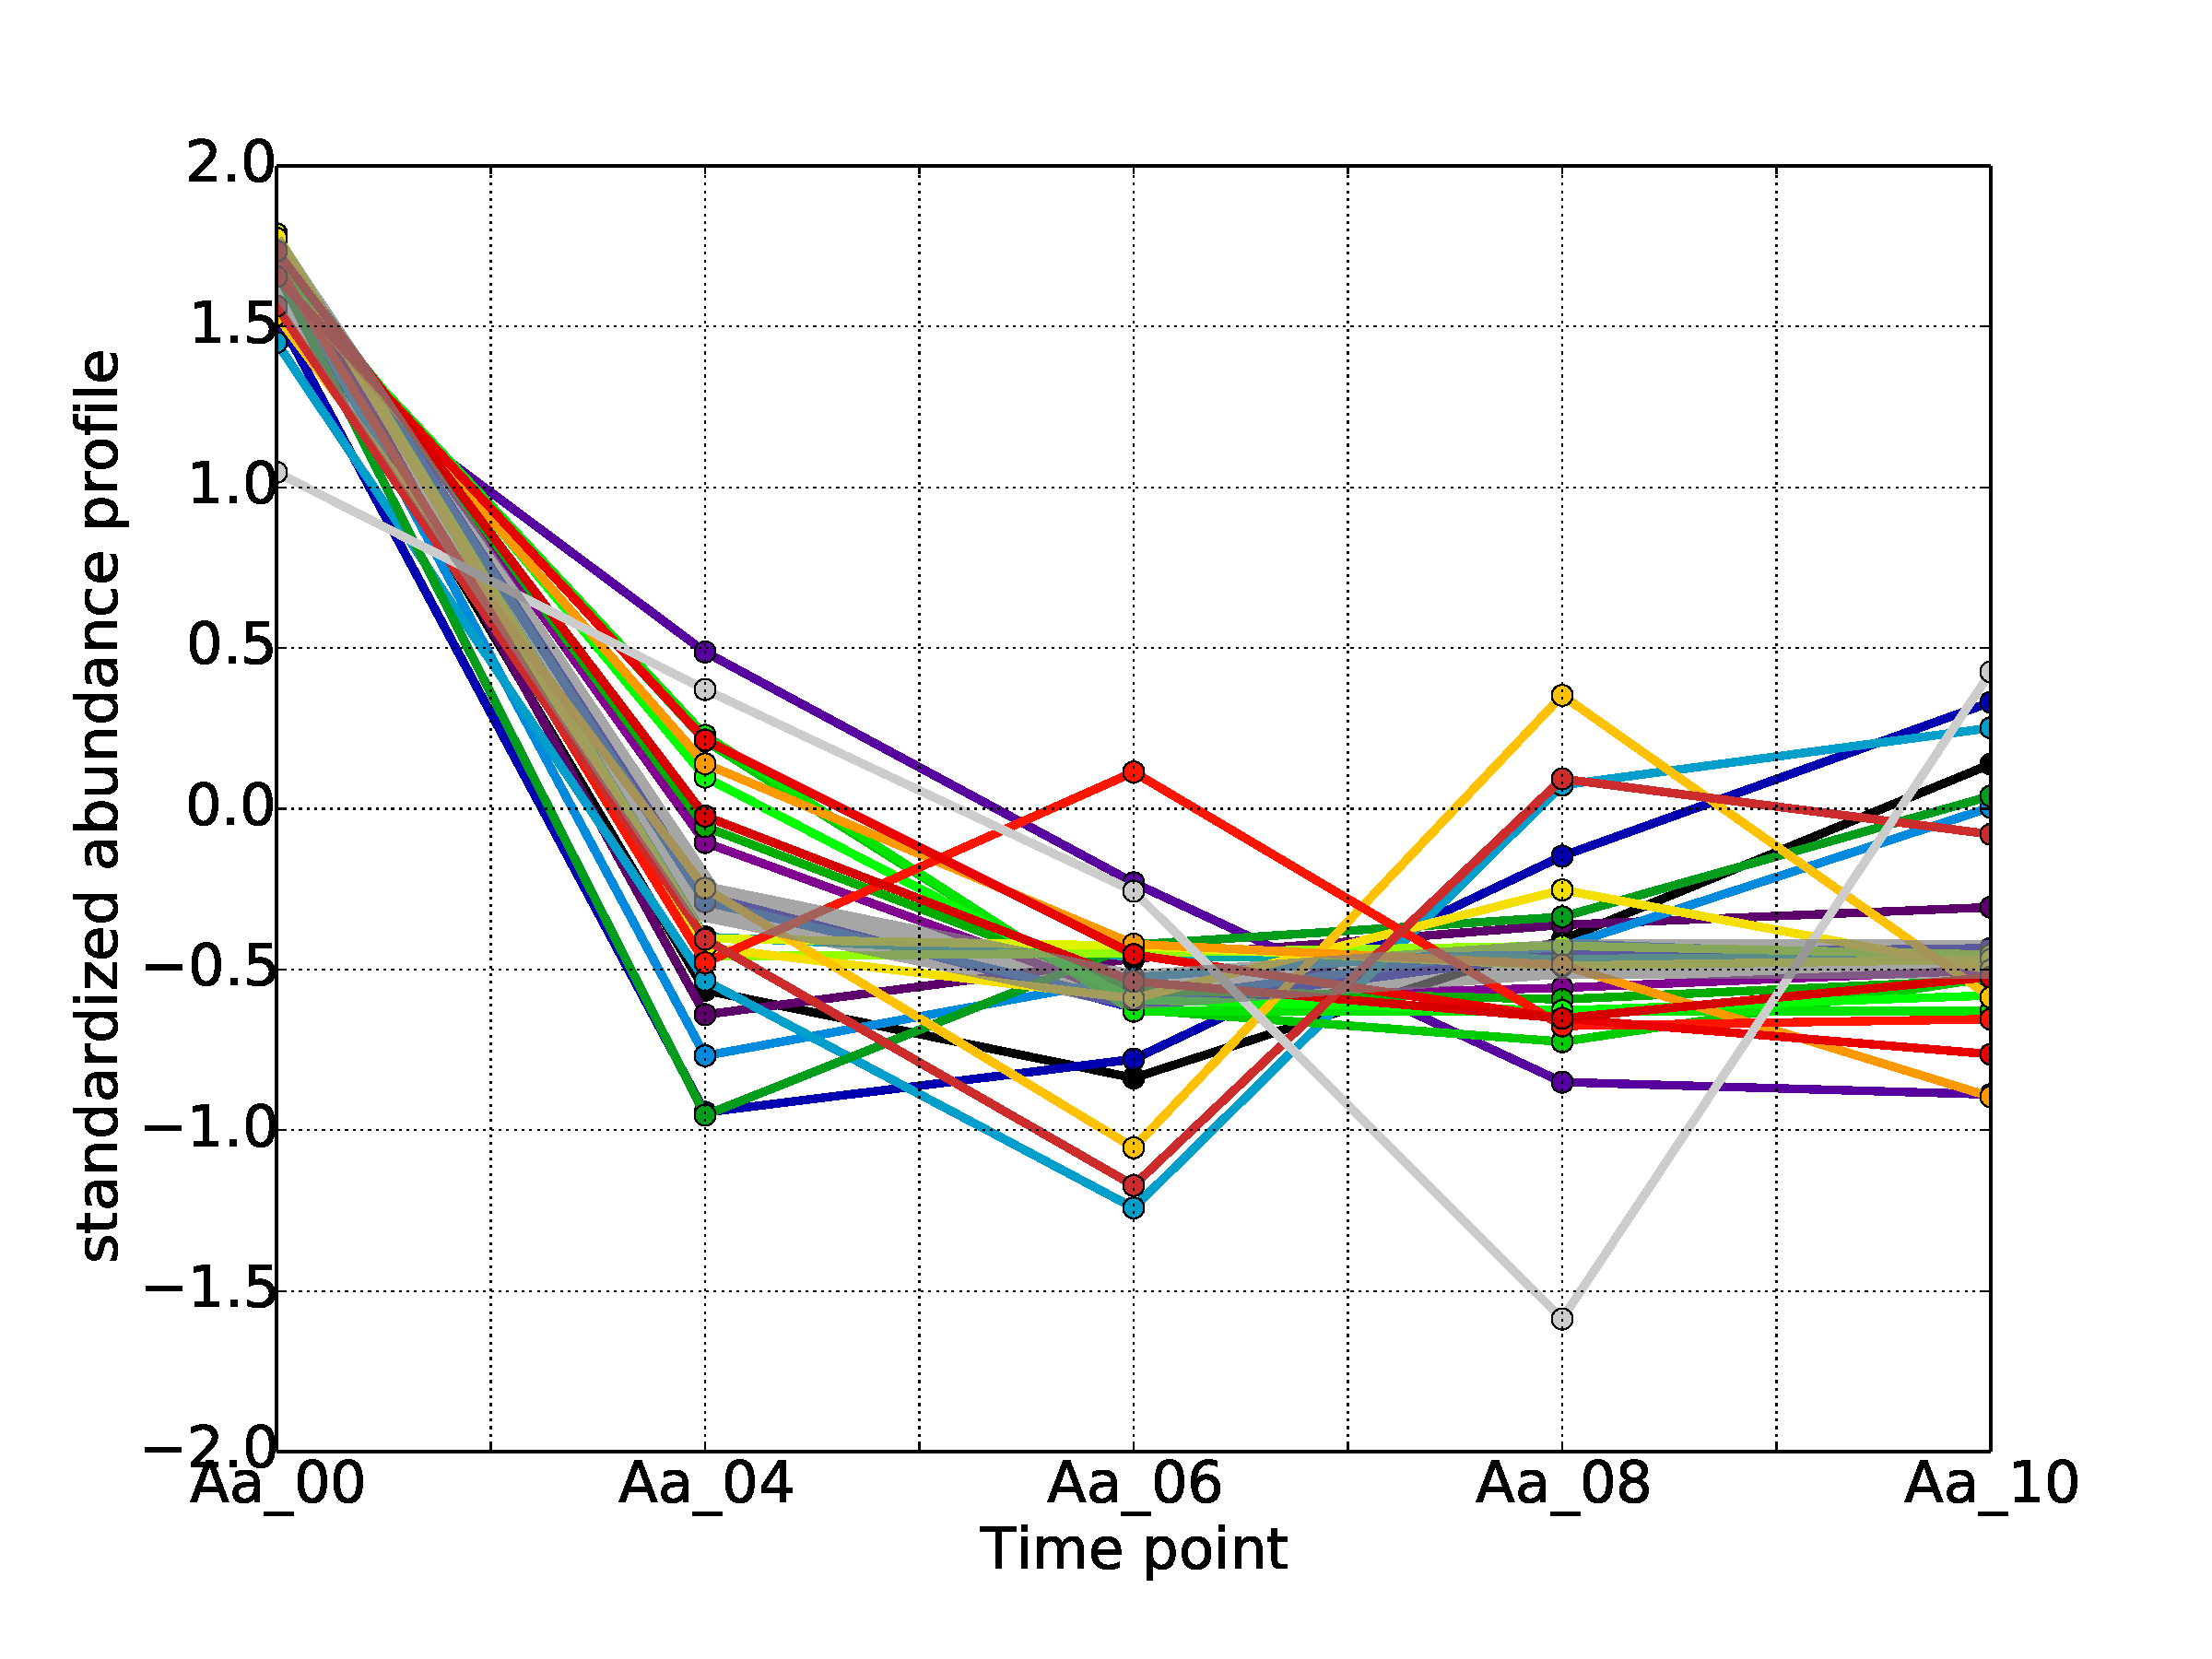
\includegraphics[width=.5\linewidth]{figures/figs/ecr_and_insects_ptci_20130918_orthodb7/downAfter4_gene_profiles_from_cummerbund/Aa_downAfter4_cls6_Ag_target_FPKMs_vb_orthos.pdf}}
%
\subcaptionbox{\label{fig:cluster6-Ag}}
{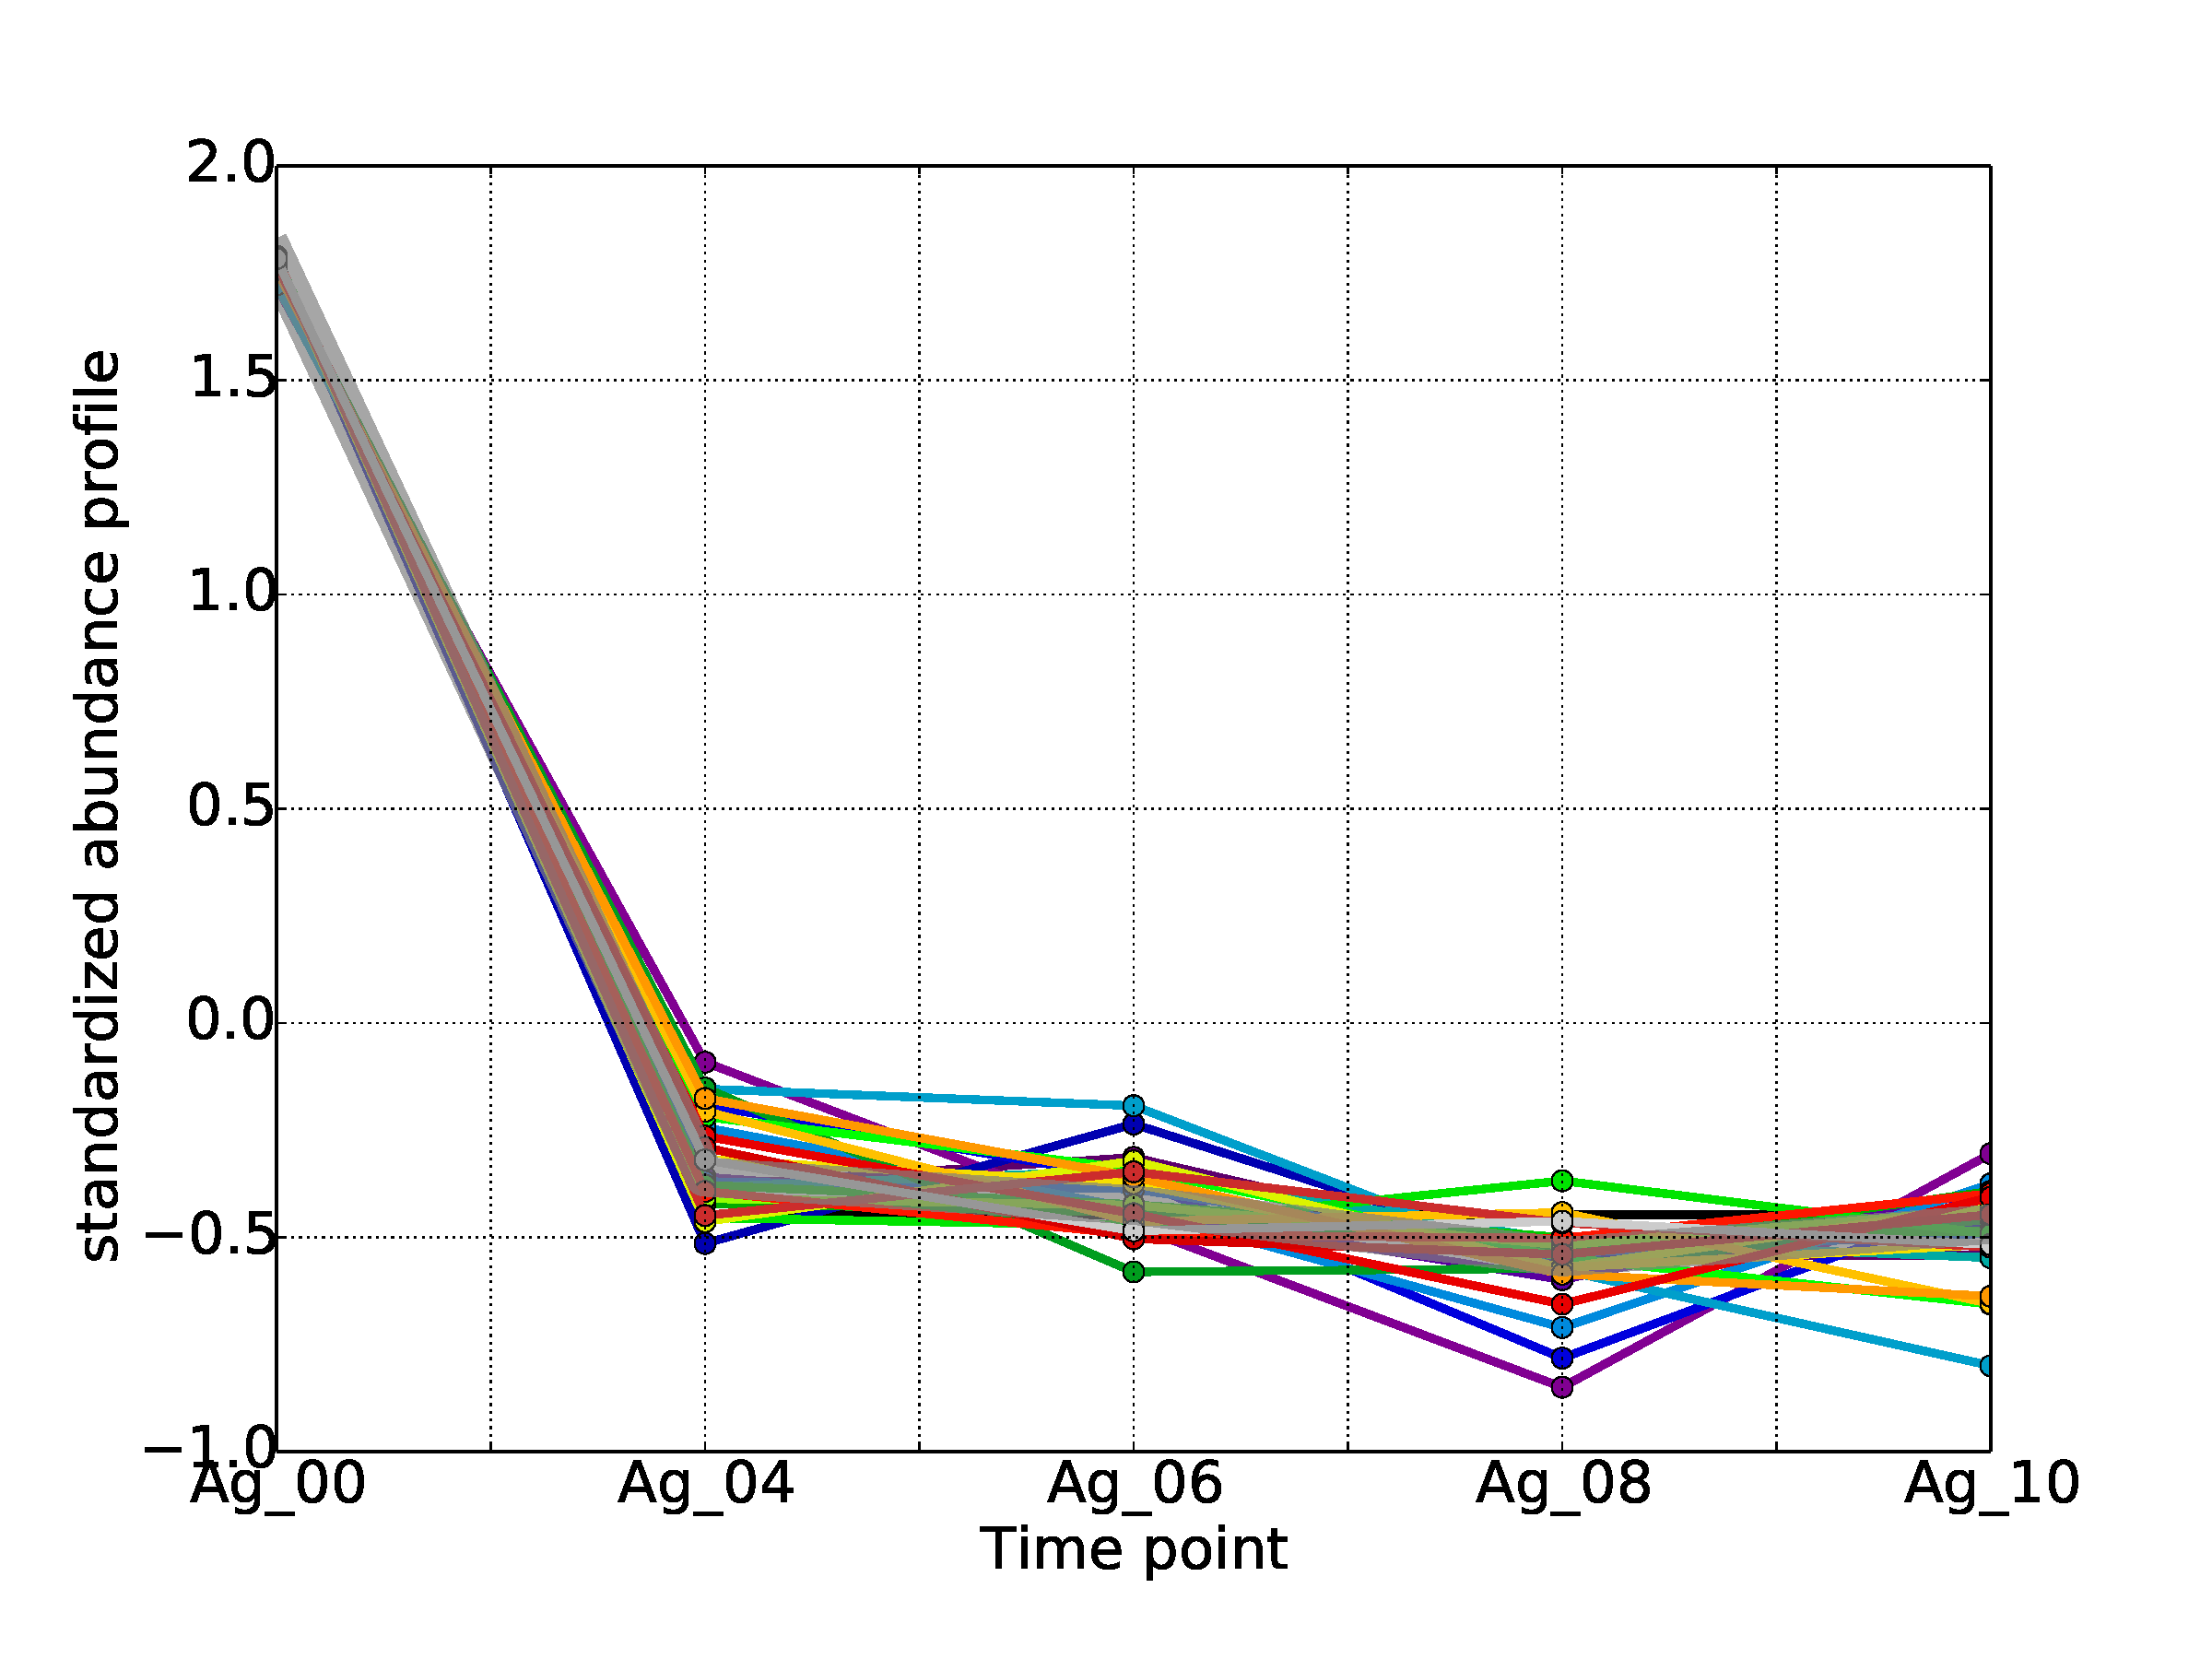
\includegraphics[width=.5\linewidth]{figures/figs/ecr_and_insects_ptci_20130918_orthodb7/downAfter4_gene_profiles_from_cummerbund/Ag_downAfter4_cls6_Ag_target_FPKMs_vb_orthos.pdf}}
%
\subcaptionbox{\label{fig:cluster6-Cq}}
{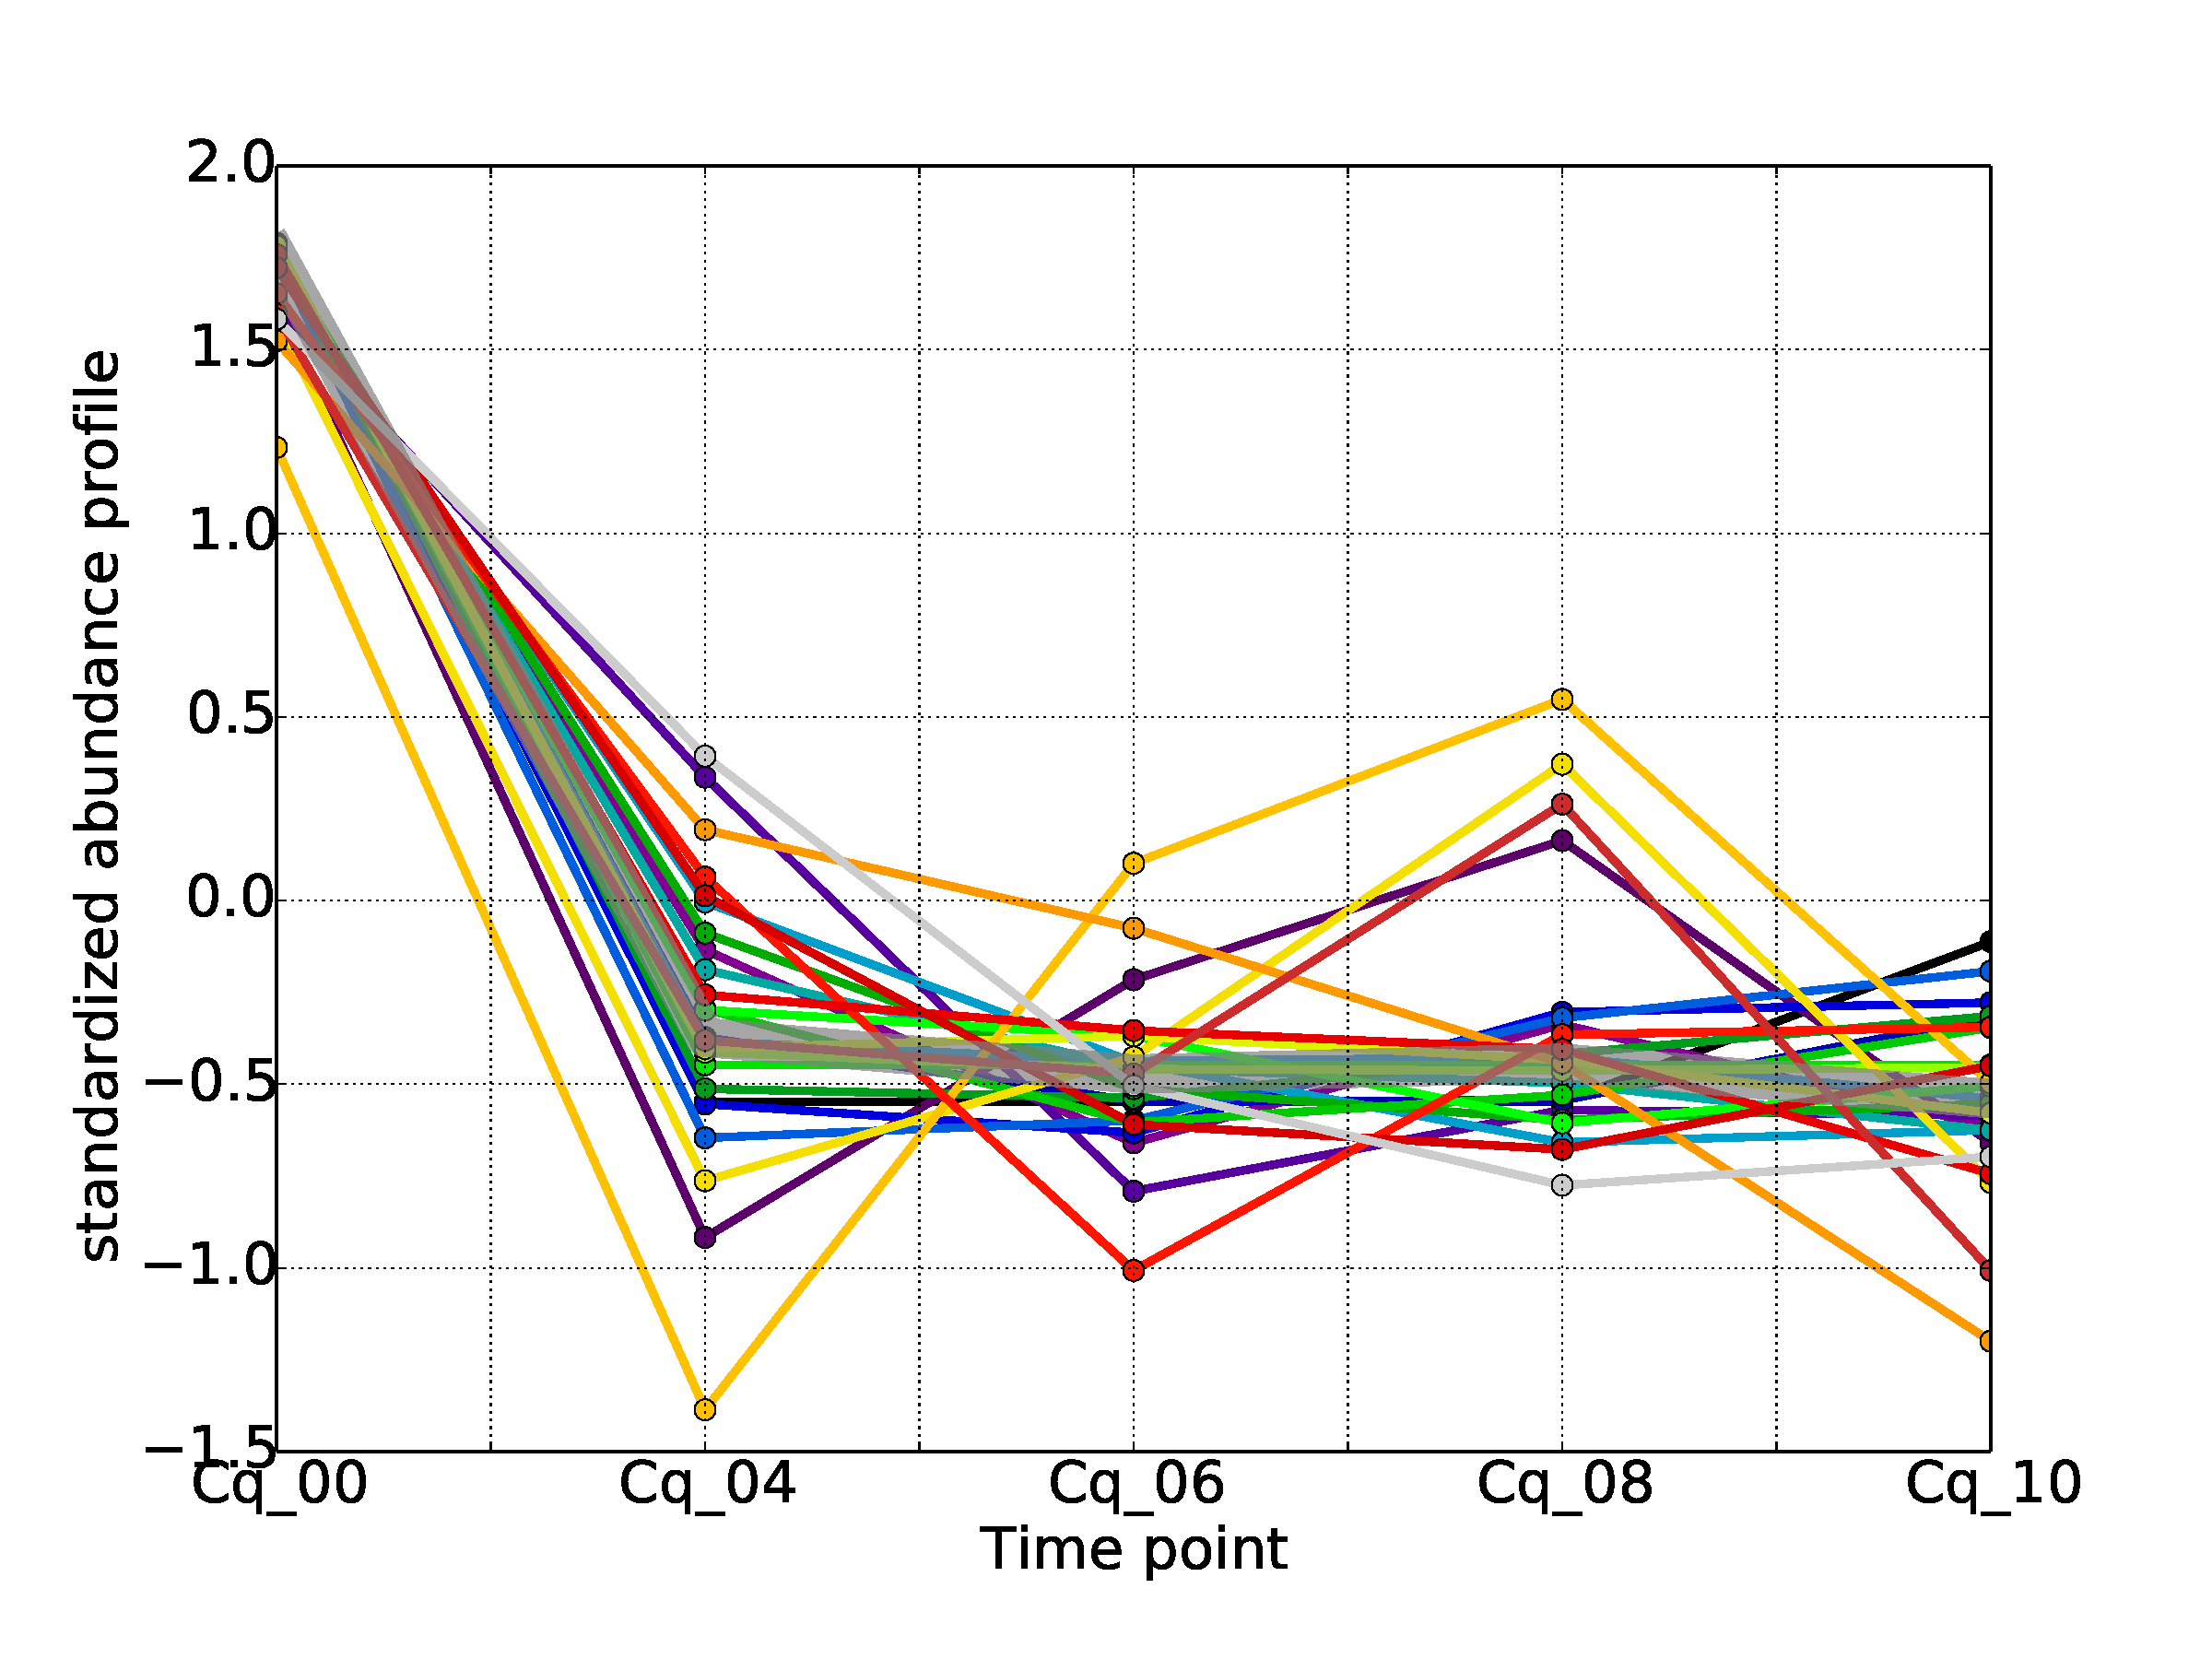
\includegraphics[width=.5\linewidth]{figures/figs/ecr_and_insects_ptci_20130918_orthodb7/downAfter4_gene_profiles_from_cummerbund/Cq_downAfter4_cls6_Ag_target_FPKMs_vb_orthos.pdf}}
% 
\caption[Orthologs of cluster 6]{\sf \textbf{Orthologs of cluster 6 (down after 4h):}\\
The same color scheme is used for each species which means that orthologs are given the same color in all three panels.
The thick, transparent gray line represents the median \gls{mAP} for the panel.
\textbf{(A)} \Aa.
\textbf{(B)} \Ag.
\textbf{(C)} \Cq.
}\label{fig:cluster6}
\end{figure}


\paragraph*{Functional annotations of cluster 6:}

% downregulation of transcription factors
% translation elongation
% signaling
% Heme management


% transcription factors
%	X AGAP002238:AAEL010222CPIJ008350 {GATA-type}
%	x AAEL009171:CPIJ001396:AGAP003726 {ortholog to Dmel bZIP family. CREBRF subfamily}
%	x CPIJ004057:AAEL009114:AGAP004050 {Doublesex}
%	x CPIJ014945:AAEL002062:AGAP005661 {Ftz-f1}
%	x AAEL001361:AGAP006990:CPIJ002241 {Bap 170 }
%	x CPIJ005607:AAEL005452:AGAP010201 {ortholog to Dmel crp}


Possible themes regarding the functional annotation terms for cluster 6 are down-regulation of certain transcription factors, signaling molecules, and heme management (Tables \ref{tab:cls6-process} and \ref{tab:cls6-function}).
% Booktabs require to add \usepackage{booktabs} to your document preamble
\begin{table}[hp]
\begin{center} \sf
\begin{tabular}{p{.7\textwidth}r}
\toprule
\textbf{Name}                                                           & \textbf{Total Score (mean)} \\ \midrule
Mo-molybdopterin cofactor biosynthetic process                          & 7762.64                     \\ % #LOOKUP
GTP catabolic process                                                   & 5712.72                     \\
translational elongation                                                & 3558.74                     \\
heme biosynthetic process                                               & 2615.06                     \\ % heme managment
glutamate biosynthetic process                                          & 2418.17                     \\
protein export from nucleus                                             & 2157.87                     \\
translation                                                             & 1962.19                     \\ % translation
cellular amino acid biosynthetic process                                & 1737.45                     \\
sex differentiation                                                     & 1549.60                     \\ % #EXPLAIN this is DBX
nuclear-transcribed mRNA catabolic process, nonsense-mediated decay     & 1190.98                     \\ % #LOOKUP
biosynthetic process                                                    & 1116.03                     \\
regulation of cyclin-dependent protein serine/threonine kinase activity & 950.21                      \\ % #LOOKUP CyclinT
cell adhesion                                                           & 938.98                      \\
intracellular protein transport                                         & 853.03                      \\
glutamine metabolic process                                             & 826.49                      \\
steroid hormone mediated signaling pathway                              & 779.04                      \\ % #LOOKUP (AGAP005661:AAEL002062:CPIJ014945 Ftz transcription factor)
protoporphyrinogen IX biosynthetic process                              & 769.19                      \\ % #LOOKUP Heme Biosynth
regulation of transcription, DNA-dependent                              & 760.48                      \\ 
nitrogen compound metabolic process                                     & 726.25                      \\
rRNA processing                                                         & 660.29                      \\
SRP-dependent cotranslational protein targeting to membrane             & 653.41                      \\
tetrapyrrole biosynthetic process                                       & 607.64                      \\
ribosome biogenesis                                                     & 571.22                      \\
transport                                                               & 489.46                      \\
transcription, DNA-dependent                                            & 454.23                      \\
protein transport                                                       & 449.05                      \\
cell-matrix adhesion                                                    & 339.59                      \\
Wnt receptor signaling pathway                                          & 330.08                      \\
nucleosome disassembly                                                  & 285.68                      \\ % 1:1 ortho of Dmel: Brahma associated protein 170kD [Bap170]
actin filament bundle assembly                                          & 281.75                      \\
metabolic process                                                       & 270.58                      \\
protein phosphorylation                                                 & 263.56                      \\
enzyme active site formation via L-cysteine persulfide                  & 228.92                      \\
synapse assembly                                                        & 222.33                      \\
regulation of protein export from nucleus                               & 214.34                      \\
neurogenesis                                                            & 212.84                      \\ \bottomrule
\end{tabular}
\end{center}

\caption[Cluster 6 top process GO terms]{\sf \textbf{Cluster 6 top process GO terms}}
\label{tab:cls6-process}
\end{table}
% Booktabs require to add \usepackage{booktabs} to your document preamble
\begin{table}[h]
\begin{center} \sf
\begin{tabular}{p{.7\textwidth}r}
\toprule
\textbf{Name}                                                 & \textbf{Total Score (mean)} \\ \midrule
protein transporter activity                                  & 9225.37                     \\
translation elongation factor activity                        & 4478.17                     \\ % #EXPLAIN
GTPase activity                                               & 4364.13                     \\
GTP binding                                                   & 3823.91                     \\
phospholipid binding                                          & 3341.66                     \\
pyridoxal phosphate binding                                   & 2871.76                     \\
steroid hormone receptor activity                             & 2322.77                     \\ % which gene(s) is this?
protein kinase binding                                        & 2059.25                     \\
sequence-specific DNA binding                                 & 1999.76                     \\ % transcription factor repression?
protein N-terminus binding                                    & 1781.39                     \\
protein complex binding                                       & 1446.01                     \\
transferase activity, transferring acyl groups                & 1047.27                     \\
integrin binding                                              & 1003.53                     \\
protein domain specific binding                               & 995.27                      \\
DNA binding                                                   & 910.28                      \\ % transcription factor repression?
ATP-dependent helicase activity                               & 877.71                      \\
carboxylesterase activity                                     & 828.49                      \\
sequence-specific DNA binding transcription factor activity   & 796.99                      \\ % transcription factor repression?
nucleotide binding                                            & 772.48                      \\ % transcription factor repression?
hydrolase activity                                            & 766.78                      \\
helicase activity                                             & 737.95                      \\ % #EXPLAIN
ATP binding                                                   & 700.66                      \\
glutamate synthase activity                                   & 578.54                      \\
zinc ion binding                                              & 578.26                      \\ % transcription factor repression?
protein binding                                               & 569.78                      \\
GTPase regulator activity                                     & 568.11                      \\
transferase activity                                          & 536.16                      \\
oxidoreductase activity                                       & 512.70                      \\
protein dimerization activity                                 & 503.19                      \\
nucleic acid binding                                          & 500.17                      \\
oxidoreductase activity, acting on the CH-NH2 group of donors & 461.69                      \\
metal ion binding                                             & 453.98                      \\
kinesin binding                                               & 450.65                      \\
JUN kinase binding                                            & 392.02                      \\ % #EXPLAIN
phosphatidylinositol-3,4,5-trisphosphate binding              & 387.10                      \\
lipid binding                                                 & 367.29                      \\
RNA binding                                                   & 316.90                      \\
protein homodimerization activity                             & 309.12                      \\ % transcription factor repression?
catalytic activity                                            & 263.32                      \\
glutamate synthase (ferredoxin) activity                      & 254.70                      \\ % #EXPLAIN
transporter activity                                          & 233.90                      \\ \bottomrule
\end{tabular}
\end{center}

\caption[Cluster 6 top function GO terms]{\sf \textbf{Cluster 6 top function GO terms}}
\label{tab:cls6-function}
\end{table}


At least six 3-way 1:1 ortholog sets in this cluster are likely transcription factors (Table \ref{tab:TFs-in-cls6}).
\begin{table}[hp]
\sf
\begin{center}
\begin{tabular}{lr}\toprule
\textbf{Ortholog set} & \textbf{Description} \\
\midrule
AAEL010222 & \multirow{3}{*}{GATA-type}\\
AGAP002238 & \\
CPIJ008350 & \\ \midrule
AGAP004050 & \multirow{3}{*}{doublesex}\\
AAEL009114 & \\
CPIJ004057 & \\ \midrule
AGAP005661 & \multirow{3}{*}{Ftz-F1}\\
AAEL002062 & \\
CPIJ014945 & \\ \midrule
AAEL009171 & \multirow{3}{*}{uncharacterized basic leucine zipper (CREBRF subfamily)}\\
AGAP003726 & \\
CPIJ001396 & \\ \midrule
AAEL001361 & \multirow{3}{*}{ortholog of \Dm\ Brahma associated protein 170kD (Bap170)}\\
AGAP006990 & \\
CPIJ002241 & \\ \midrule
AAEL005452 & \multirow{3}{*}{ortholog of \Dm\ cropped (crp)}\\
AGAP010201 & \\
CPIJ005607 & \\ \bottomrule
\end{tabular}
\end{center}

\caption[Transcription factors in cluster 6 (down after 4h)]{\sf \textbf{Transcription factors in cluster 6 (down after 4h)}} \label{tab:TFs-in-cls6}
\end{table} 
%
Five have putative identities based on orthology to \Dm\ or have been given the names in at least one of the mosquito genome projects on VectorBase.
%
The are a GATA-factor member, doublesex, Ftz-F1, Bap 170, and crp.
%
The last, which exists only as accession numbers in all species including \Dm, is predicted to be a basic leucine zipper transcription factor.

Process terms relating to signaling activities include (trailing parenthetical represents the mean \gls{TS}) regulation of cyclin-dependent protein serine/threonine kinase activity (950.21), steroid hormone mediated signaling pathway (779.04), Wnt receptor signaling pathway (330.08), protein phosphorylation (263.56), and synapse assembly (222.33).
%
Relevant function terms are steroid hormone receptor activity (2322.77), protein kinase binding (2059.25), sequence-specific DNA binding (1999.76), integrin binding (1003.53), JUN kinase binding (392.02), and phosphatidylinositol-3,4,5-trisphosphate binding (387.10).

Another notable set of annotation terms concerns heme management.
%
They are heme biosynthetic process (2615.06), protoporphyrinogen IX biosynthetic process (769.19), tetrapyrrole biosynthetic process (607.64), and pyridoxal phosphate binding (2871.76).
%
They all originate from the same ortholog-set (AAEL007787, AGAP003184, CPIJ007746), which are aminolevulinate synthases.
%
Aminolevulinate synthase catalyzes D-Aminolevulinic acid which is the first precursor in the pathway to produce heme.








\subsubsection{Cluster 16 (down at 4h)}

\paragraph*{General description:}

Cluster 16 is characterized by genes that have a median \gls{NBF} \gls{FPKM} of approximately 1.5 standard deviations \textit{above} their overall mean \gls{FPKM} and a 4h \gls{PBM} median \gls{FPKM} value of between 0.5 and 1 standard deviations \textit{below} their overall mean \gls{FPKM}. The median \gls{FPKM} values for the remaining time points then gradually approach the overall mean \gls{FPKM} by the end of the time course (Figures \ref{fig:23-clusters} and \ref{fig:cluster16}).
%
This \gls{mAP} illustrates a rapid and substantial but temporary decrease in mRNA abundance following bloodfeeding.
%
\begin{figure}[p]
% 
\subcaptionbox{\label{fig:cluster16-Aa}}
{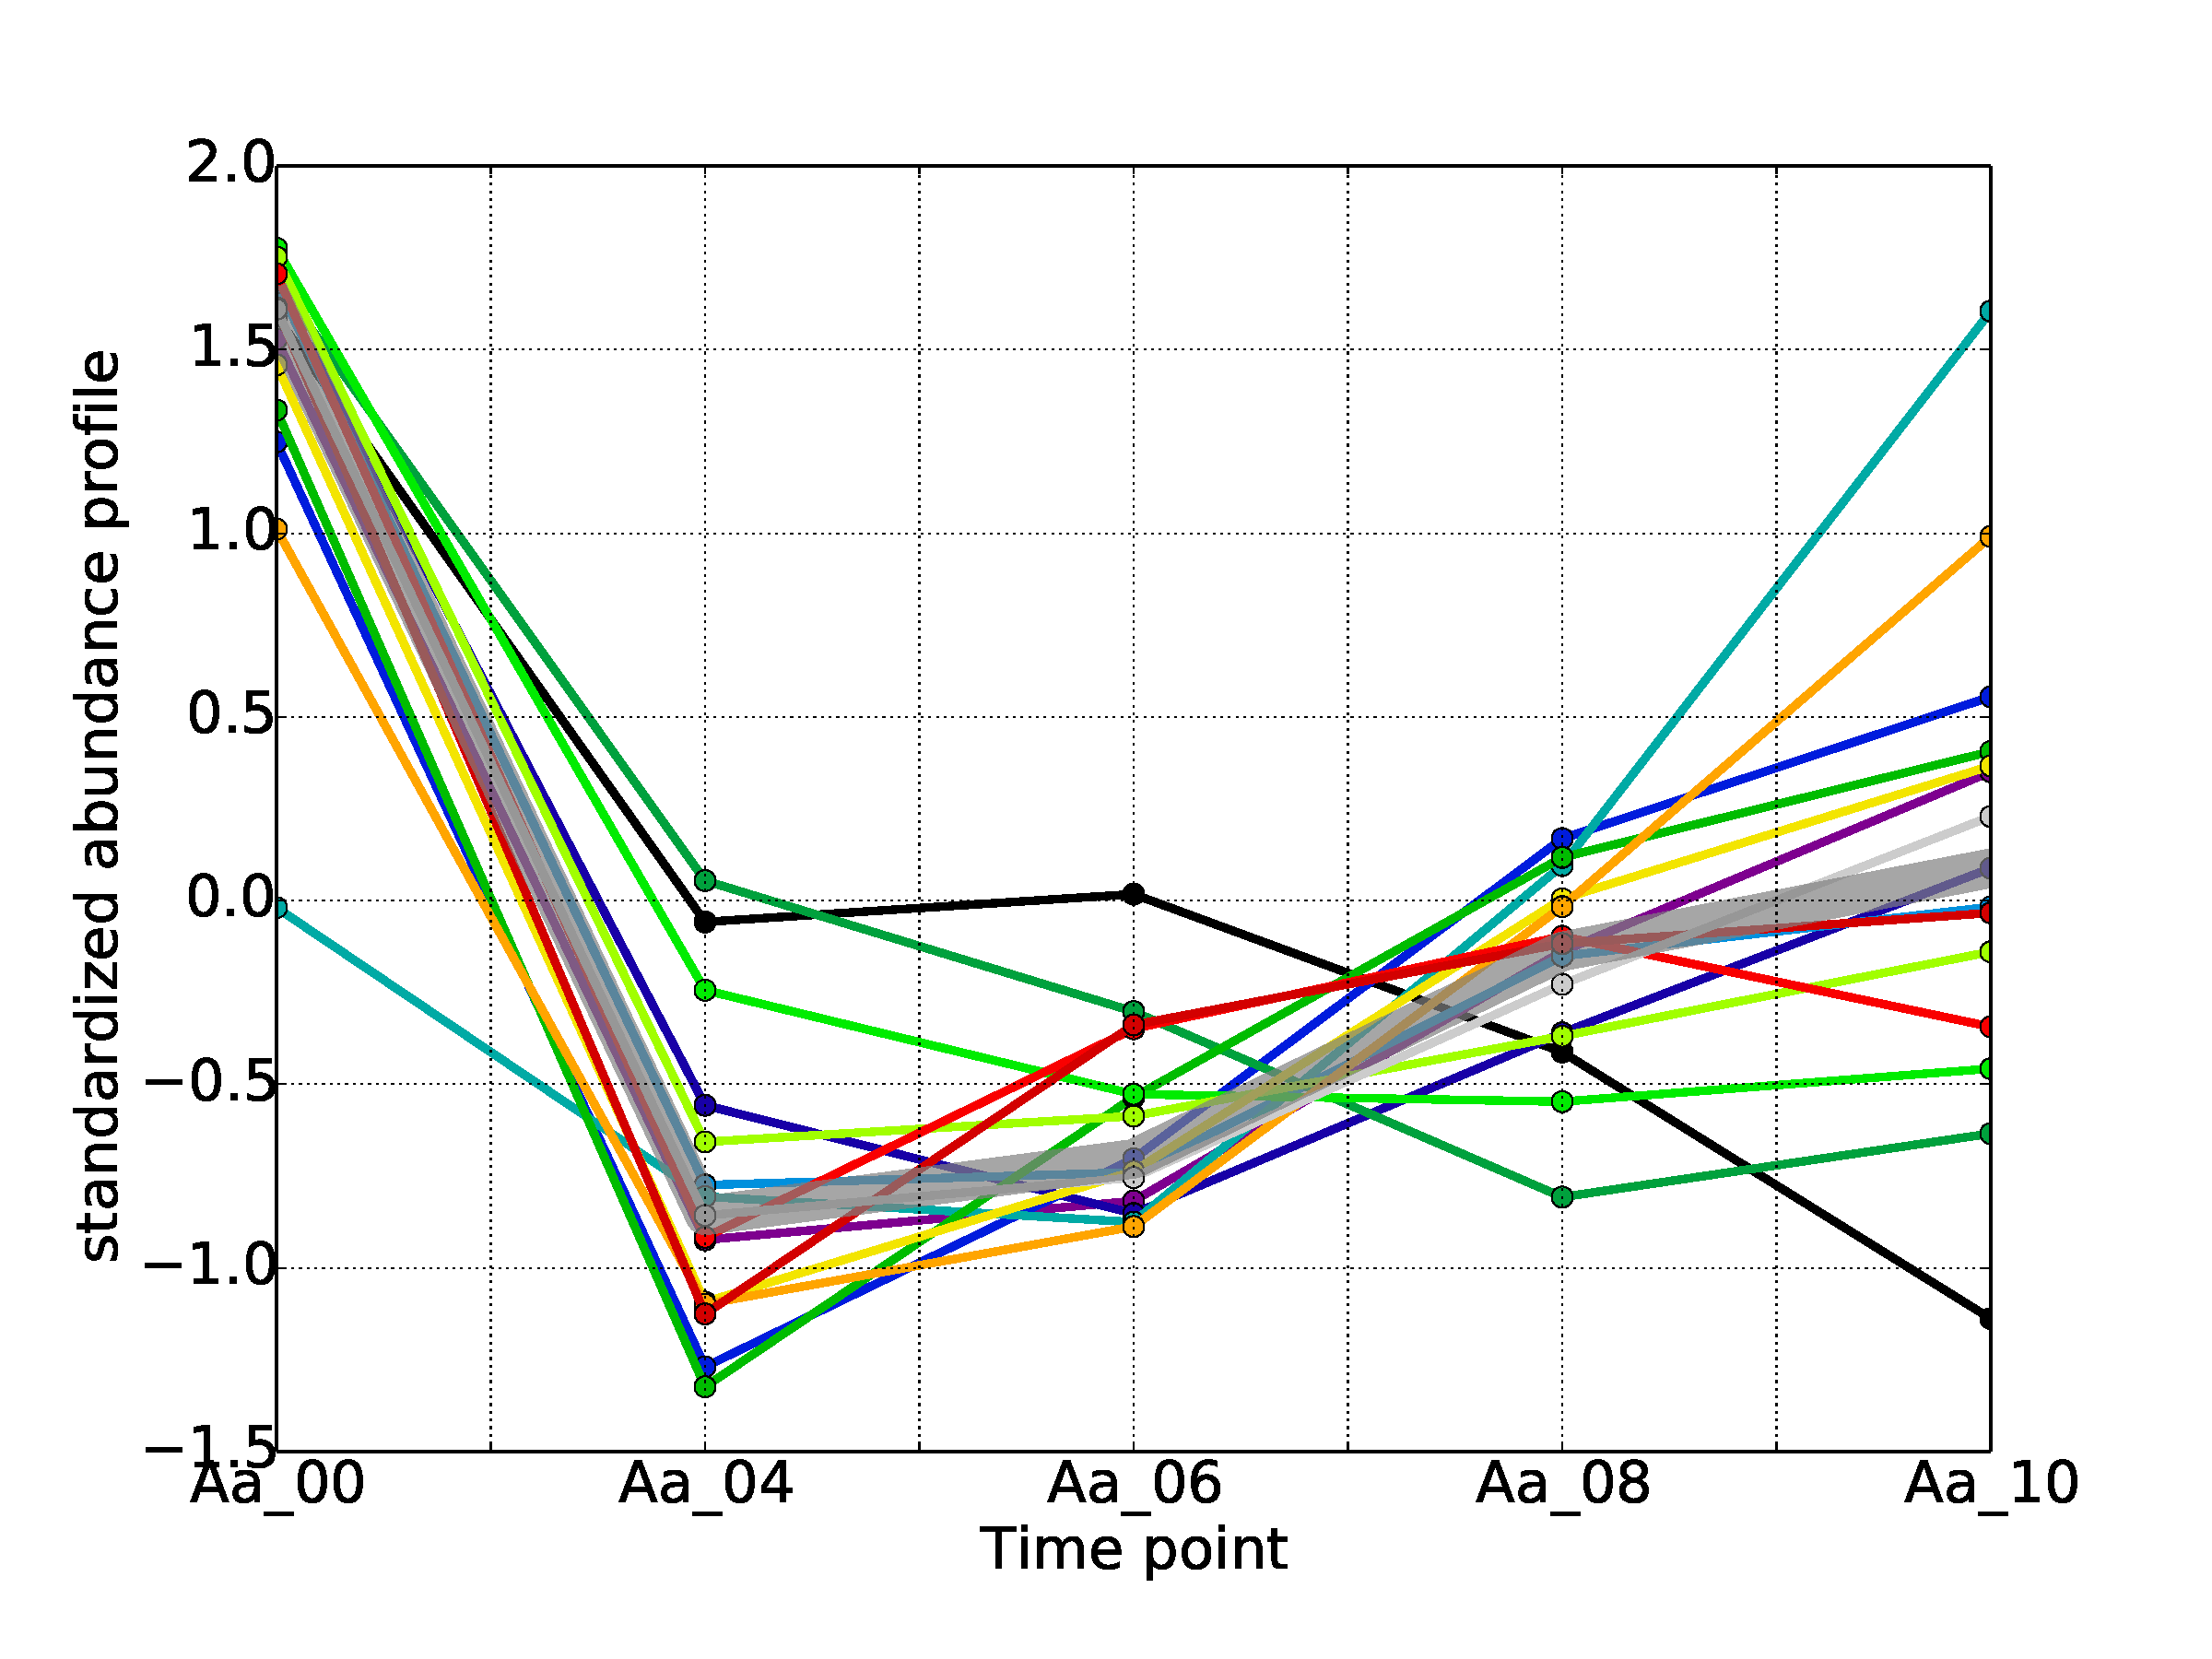
\includegraphics[width=.5\linewidth]{figures/figs/ecr_and_insects_ptci_20130918_orthodb7/downAt4_gene_profiles_from_cummerbund/Aa_downAt4_cls16_Ag_target_FPKMs_vb_orthos.pdf}}
%
\subcaptionbox{\label{fig:cluster16-Ag}}
{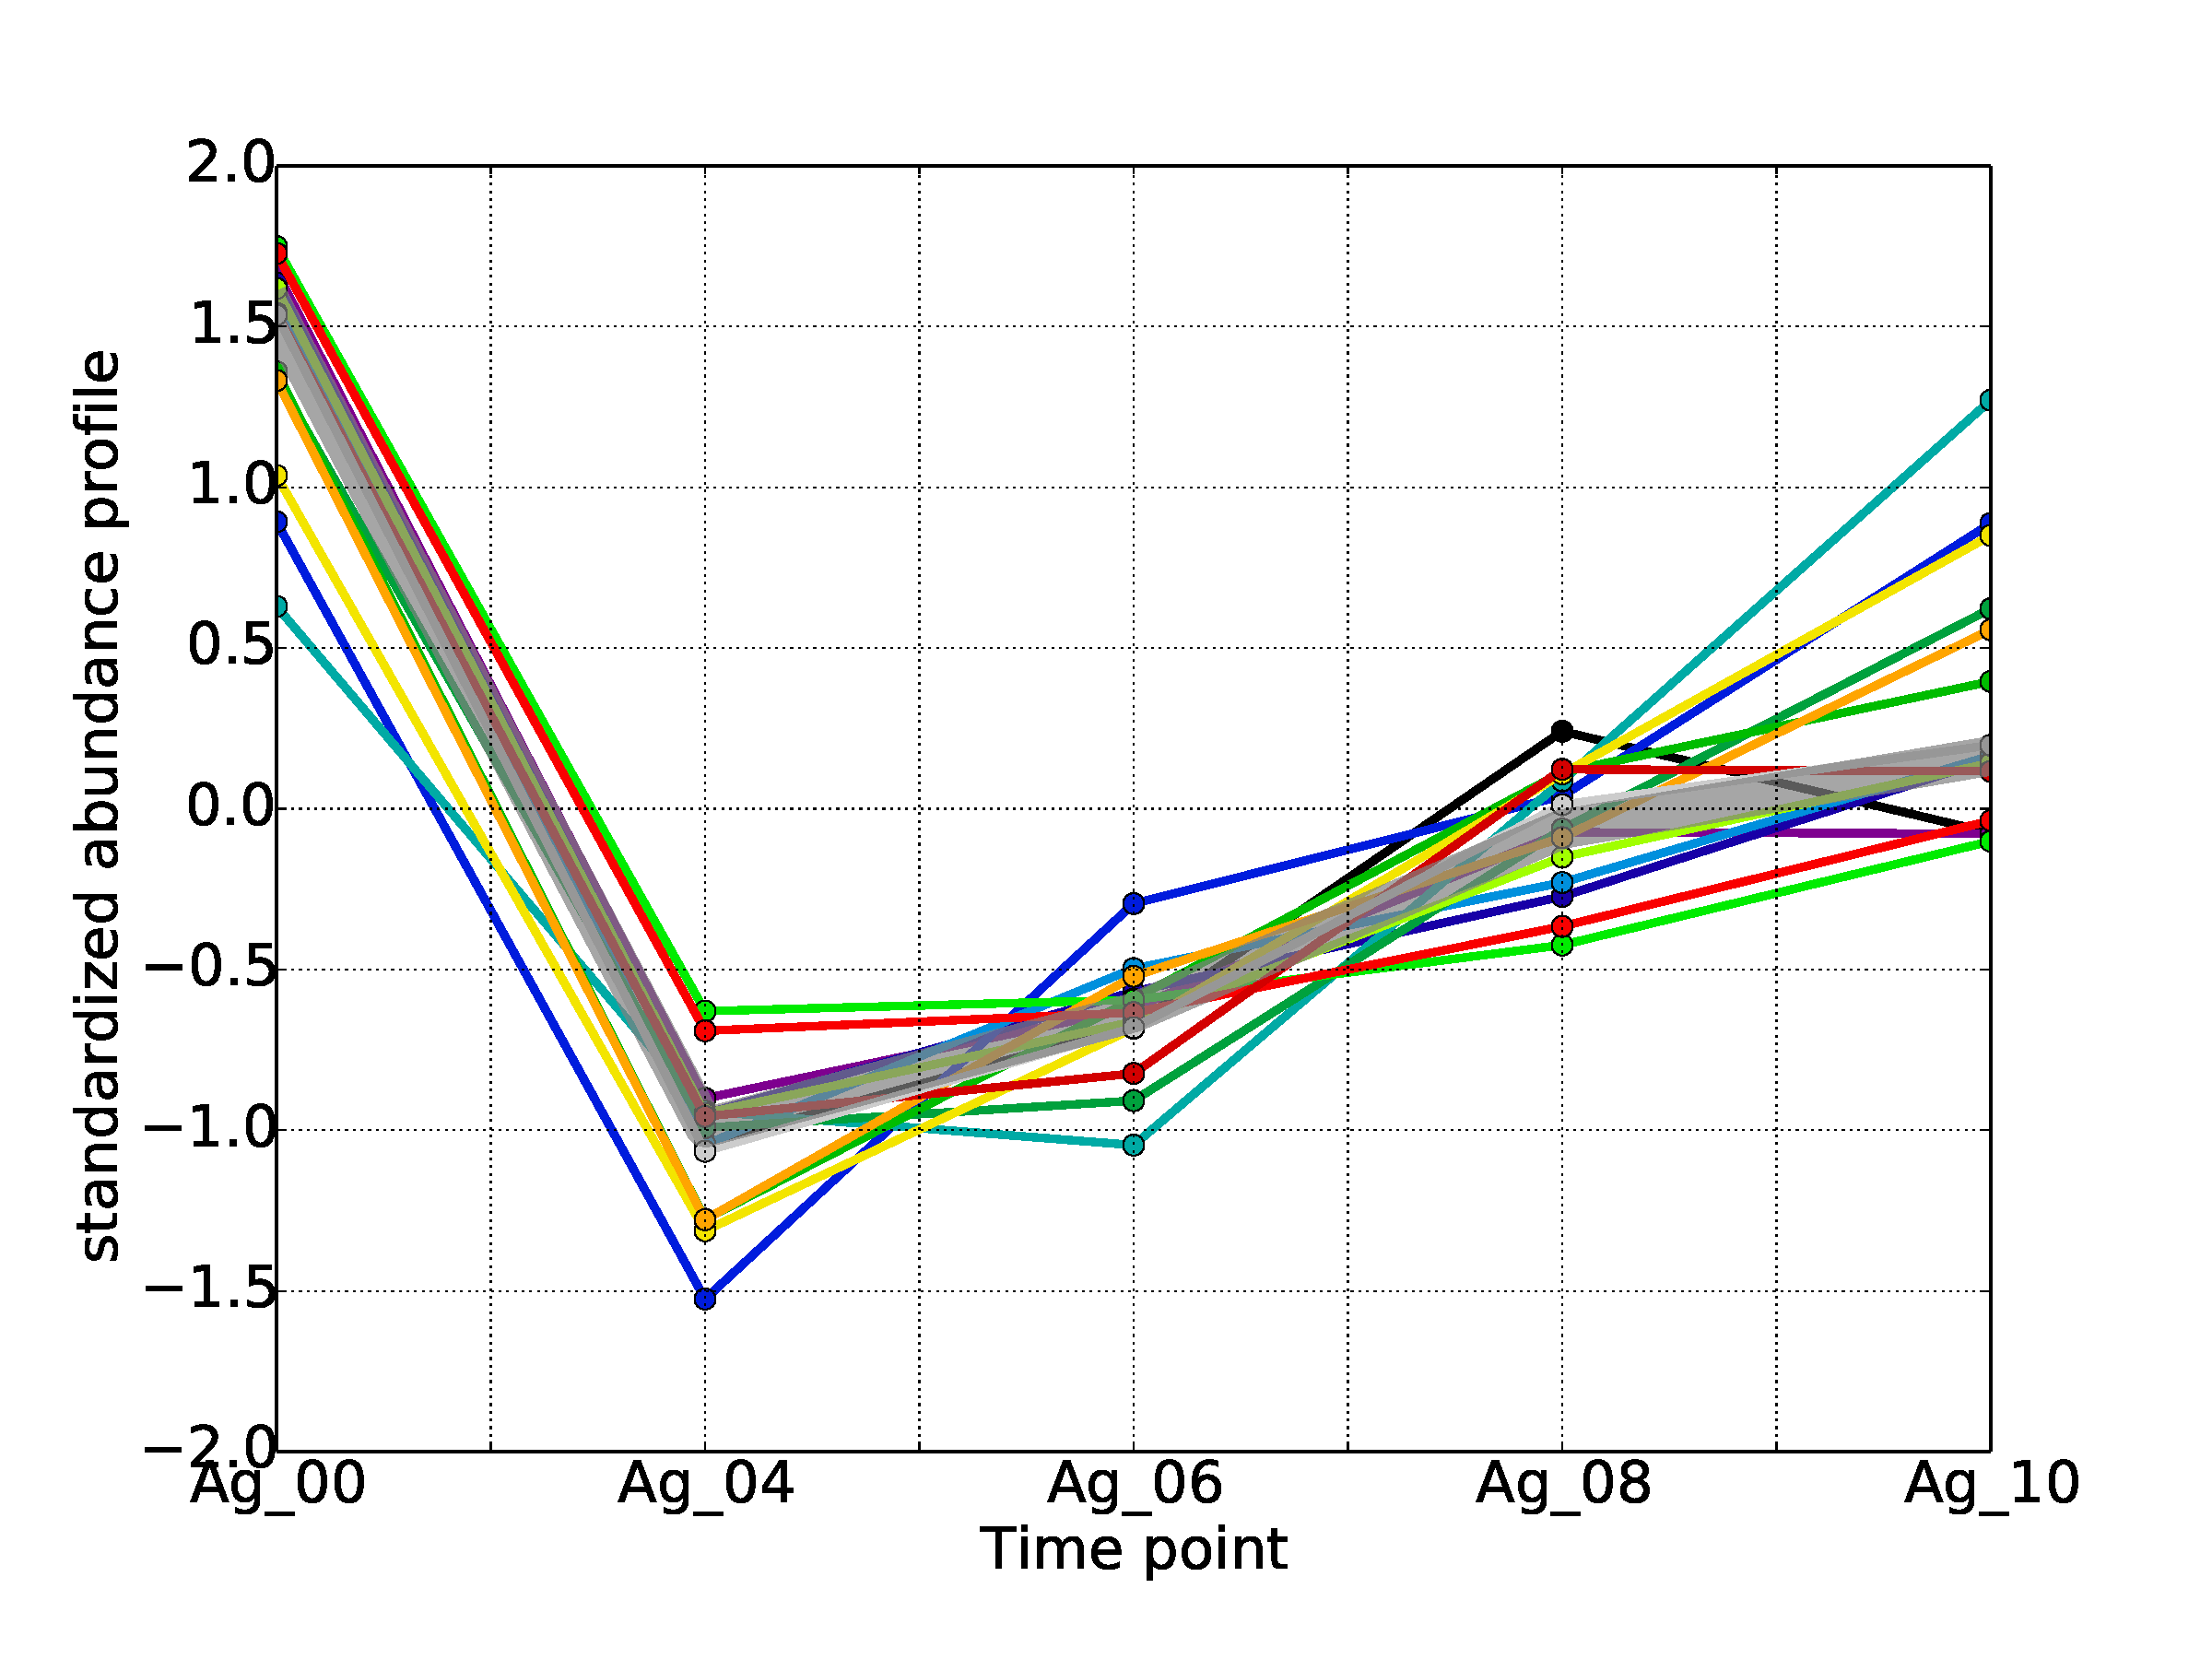
\includegraphics[width=.5\linewidth]{figures/figs/ecr_and_insects_ptci_20130918_orthodb7/downAt4_gene_profiles_from_cummerbund/Ag_downAt4_cls16_Ag_target_FPKMs_vb_orthos.pdf}}
%
\subcaptionbox{\label{fig:cluster16-Cq}}
{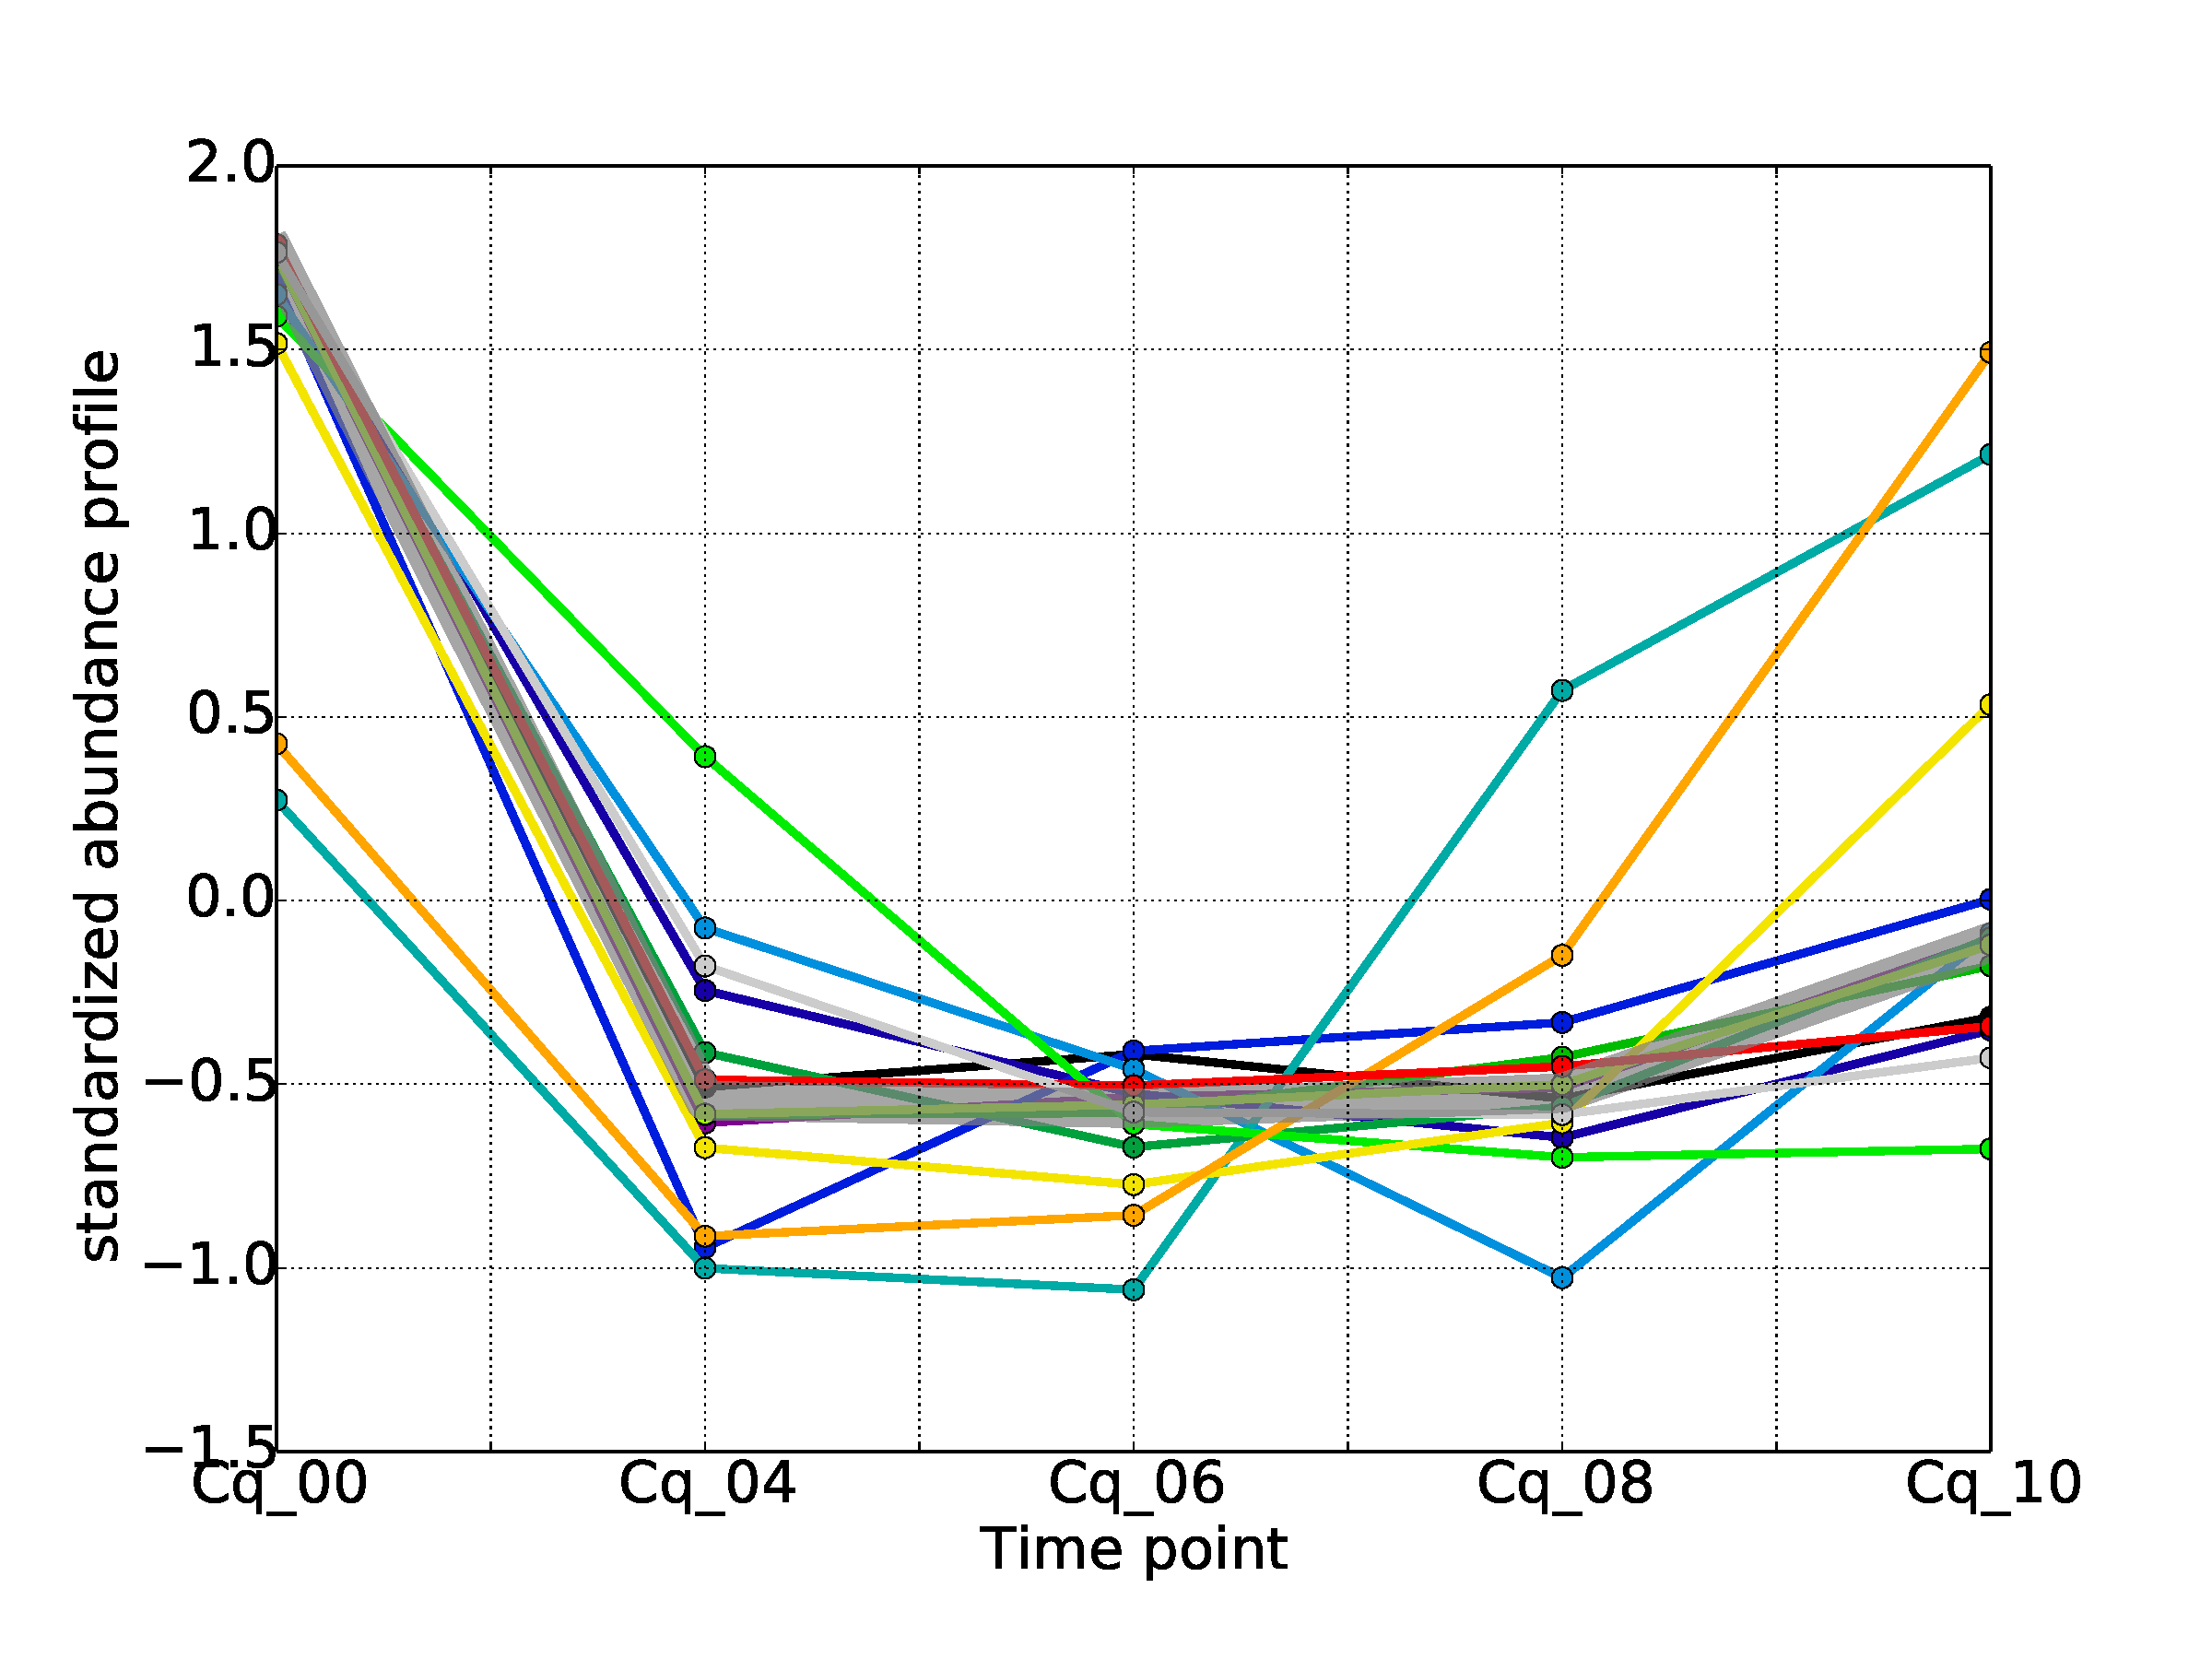
\includegraphics[width=.5\linewidth]{figures/figs/ecr_and_insects_ptci_20130918_orthodb7/downAt4_gene_profiles_from_cummerbund/Cq_downAt4_cls16_Ag_target_FPKMs_vb_orthos.pdf}}
% 
\caption[Orthologs of cluster 16]{\sf \textbf{Orthologs of cluster 16 (down at 4h):}\\
The same color scheme is used for each species which means that orthologs are given the same color in all three panels.
The thick, transparent gray line represents the median \gls{mAP} for the panel.
\textbf{(A)} \Aa.
\textbf{(B)} \Ag.
\textbf{(C)} \Cq.
}\label{fig:cluster16}
\end{figure}


\paragraph*{Functional annotations of cluster 16:}

% Downreulation of carbohydrate metabolism
% downregulation of autophagy/apoptotic process (yippee)/cellular arrest
% dwnreg of translation-repression
%   AAEL002550	 AGAP001639	 CPIJ002368 from OrthoDB

Cluster 16 contains genes with annotations that largely fit into the areas of carbohydrate digestion, cellular arrest, and repression of translation (Tables \ref{tab:cls16-process} and \ref{tab:cls16-process}).
%
Two ortholog-sets produced errors during the process that parsed the \gls{Argot2} results and others returned no process or function domain terms.
%
In these cases, OrthoDB was used to examine annotation terms assigned to these ortholog-sets using the OrthoDB ``metazoa'' database, and are noted as OrthoDB results.

% Booktabs require to add \usepackage{booktabs} to your document preamble
\begin{table}[h]
\begin{center} \sf
\begin{tabular}{p{.7\textwidth}r}
\toprule
\textbf{Name}                                 & \textbf{Total Score (mean)} \\ \midrule
one-carbon metabolic process                  & 8498.68                     \\
carbohydrate metabolic process                & 4077.43                     \\
translation                                   & 3505.77                     \\
regulation of Rho protein signal transduction & 1336.90                     \\
homophilic cell adhesion                      & 1316.75                     \\
cell adhesion                                 & 851.76                      \\
autophagy                                     & 686.01                      \\
apoptotic process                             & 670.22                      \\
regulation of myelination                     & 618.20                      \\
protein phosphorylation                       & 542.93                      \\
phosphorylation                               & 395.02                      \\
metabolic process                             & 286.58                      \\
protein transport                             & 262.15                      \\
protein ubiquitination                        & 242.49                      \\
intracellular signal transduction             & 212.22                      \\ \bottomrule
\end{tabular}
\end{center}

\caption[Cluster 16 top process GO terms]{\sf \textbf{Cluster 16 top process GO terms}}
\label{tab:cls16-process}
\end{table}
% Booktabs require to add \usepackage{booktabs} to your document preamble
\begin{table}[h]
\begin{center} \sf
\begin{tabular}{p{.7\textwidth}r}
\toprule
\textbf{Name}                                                    & \textbf{Total Score (mean)} \\ \midrule
carbonate dehydratase activity                                   & 4264.07                     \\
cysteine-type peptidase activity                                 & 2253.39                     \\
carbon-nitrogen ligase activity, with glutamine as amido-N-donor & 1652.90                     \\
Rho guanyl-nucleotide exchange factor activity                   & 1446.25                     \\
zinc ion binding                                                 & 1412.73                     \\
guanyl-nucleotide exchange factor activity                       & 1208.72                     \\
nucleic acid binding                                             & 810.14                      \\
peptidase activity                                               & 715.27                      \\
beta-tubulin binding                                             & 707.48                      \\
hydrolase activity, acting on glycosyl bonds                     & 652.43                      \\
glutaminyl-tRNA synthase (glutamine-hydrolyzing) activity        & 550.56                      \\
protein binding                                                  & 433.44                      \\
protein serine/threonine kinase activity                         & 413.31                      \\
metal ion binding                                                & 408.70                      \\
microtubule binding                                              & 403.62                      \\
ATP binding                                                      & 395.77                      \\
transferase activity                                             & 387.71                      \\
maltose alpha-glucosidase activity                               & 378.58                      \\
hydrolase activity                                               & 366.71                      \\
catalytic activity                                               & 331.87                      \\
ligase activity                                                  & 310.07                      \\
alpha-glucosidase activity                                       & 285.38                      \\
nucleotide binding                                               & 239.99                      \\
lyase activity                                                   & 212.94                      \\
oxidoreductase activity                                          & 206.49                      \\
protein kinase activity                                          & 200.95                      \\ \bottomrule                   
\end{tabular}
\end{center}

\caption[Cluster 16 top function GO terms]{\sf \textbf{Cluster 16 top function GO terms}}
\label{tab:cls16-function}
\end{table}

Terms relating to carbohydrate digestion are carbohydrate metabolic process (4077.43), maltose alpha-glucosidase activity (378.58), hydrolase activity (366.71), and alpha-glucosidase activity (285.38).

Cellular arrest terms assigned by \gls{Argot2} include autophagy (686.01) and apoptotic process (670.22).

%
Additionally, OrthoDB results identified one ortholog-set (AAEL002833, AGAP011828, CPIJ006471) as orthologs to \Dm\ Cathepsin L which FlyBase annotates with biological process terms including proteolysis, autophagic cell death, protein catabolic process, and salivary gland cell autophagic cell death.
%

Terms pertaining to the repression of translation were obtained from the ortholog-set including AAEL002550, AGAP001639, and CPIJ002368 via OrthoDB.
%
Process results include 32 genes with negative regulation of translational initiation (GO:0045947), and function results contain 17 genes with translation repressor activity, nucleic acid binding (GO:0000900); 15 genes with translation repressor activity (GO:0030371); and 2 genes with  poly(A) RNA binding (GO:0008143:).



\subsubsection{Cluster 22 (up at 4h)}

\paragraph*{General description:}

Cluster 22 is characterized by genes that have a median \gls{NBF} \gls{FPKM} of between 0 and 0.5 standard deviations \textit{below} their overall mean \gls{FPKM} and a 4h \gls{PBM} median \gls{FPKM} value of approximately 1.5 standard deviations \textit{above} their overall mean \gls{FPKM}. The median \gls{FPKM} values for the remaining time points then gradually approach approximately 1 standard deviations \textit{below} the overall mean \gls{FPKM} by the end of the time course (Figures \ref{fig:23-clusters} and \ref{fig:cluster22}).
%
This \gls{mAP} illustrates a rapid and substantial but temporary increase in mRNA abundance following bloodfeeding.
%
\begin{figure}[p]
% 
\subcaptionbox{\label{fig:cluster22-Aa}}
{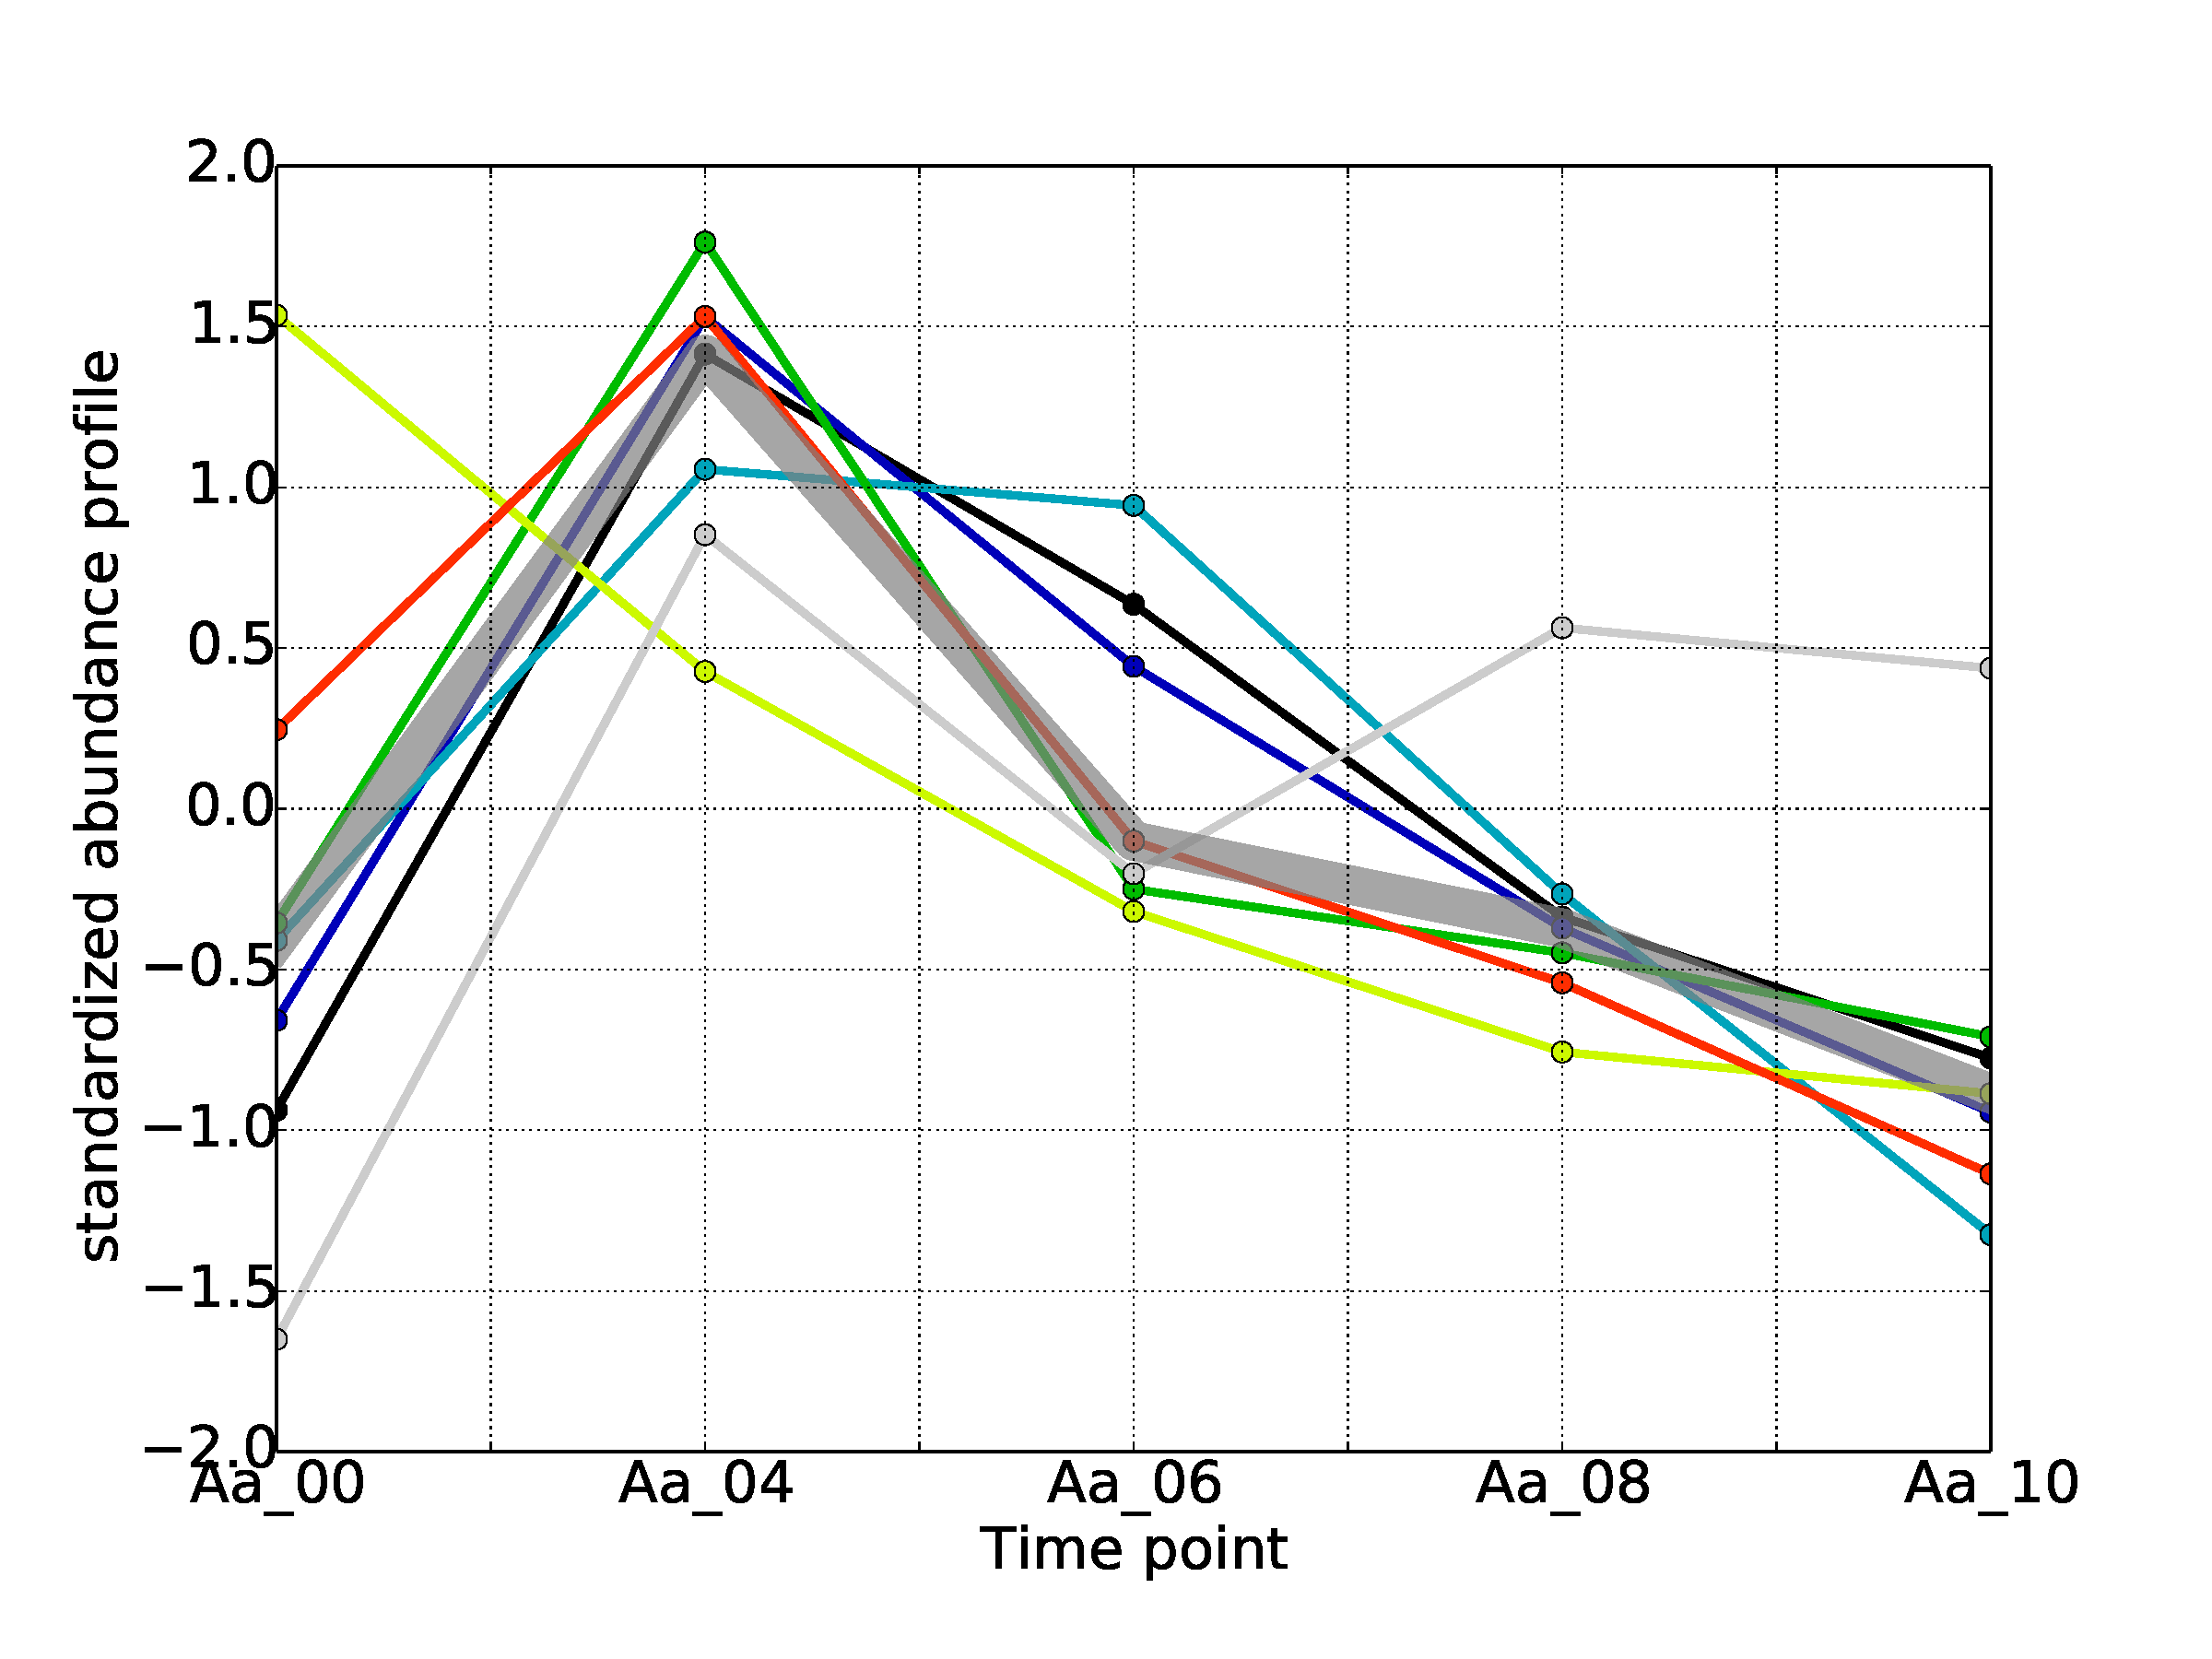
\includegraphics[width=.5\linewidth]{figures/figs/ecr_and_insects_ptci_20130918_orthodb7/upAt4_gene_profiles_from_cummerbund/Aa_upAt4_cls22_Ag_target_FPKMs_vb_orthos.pdf}}
%
\subcaptionbox{\label{fig:cluster22-Ag}}
{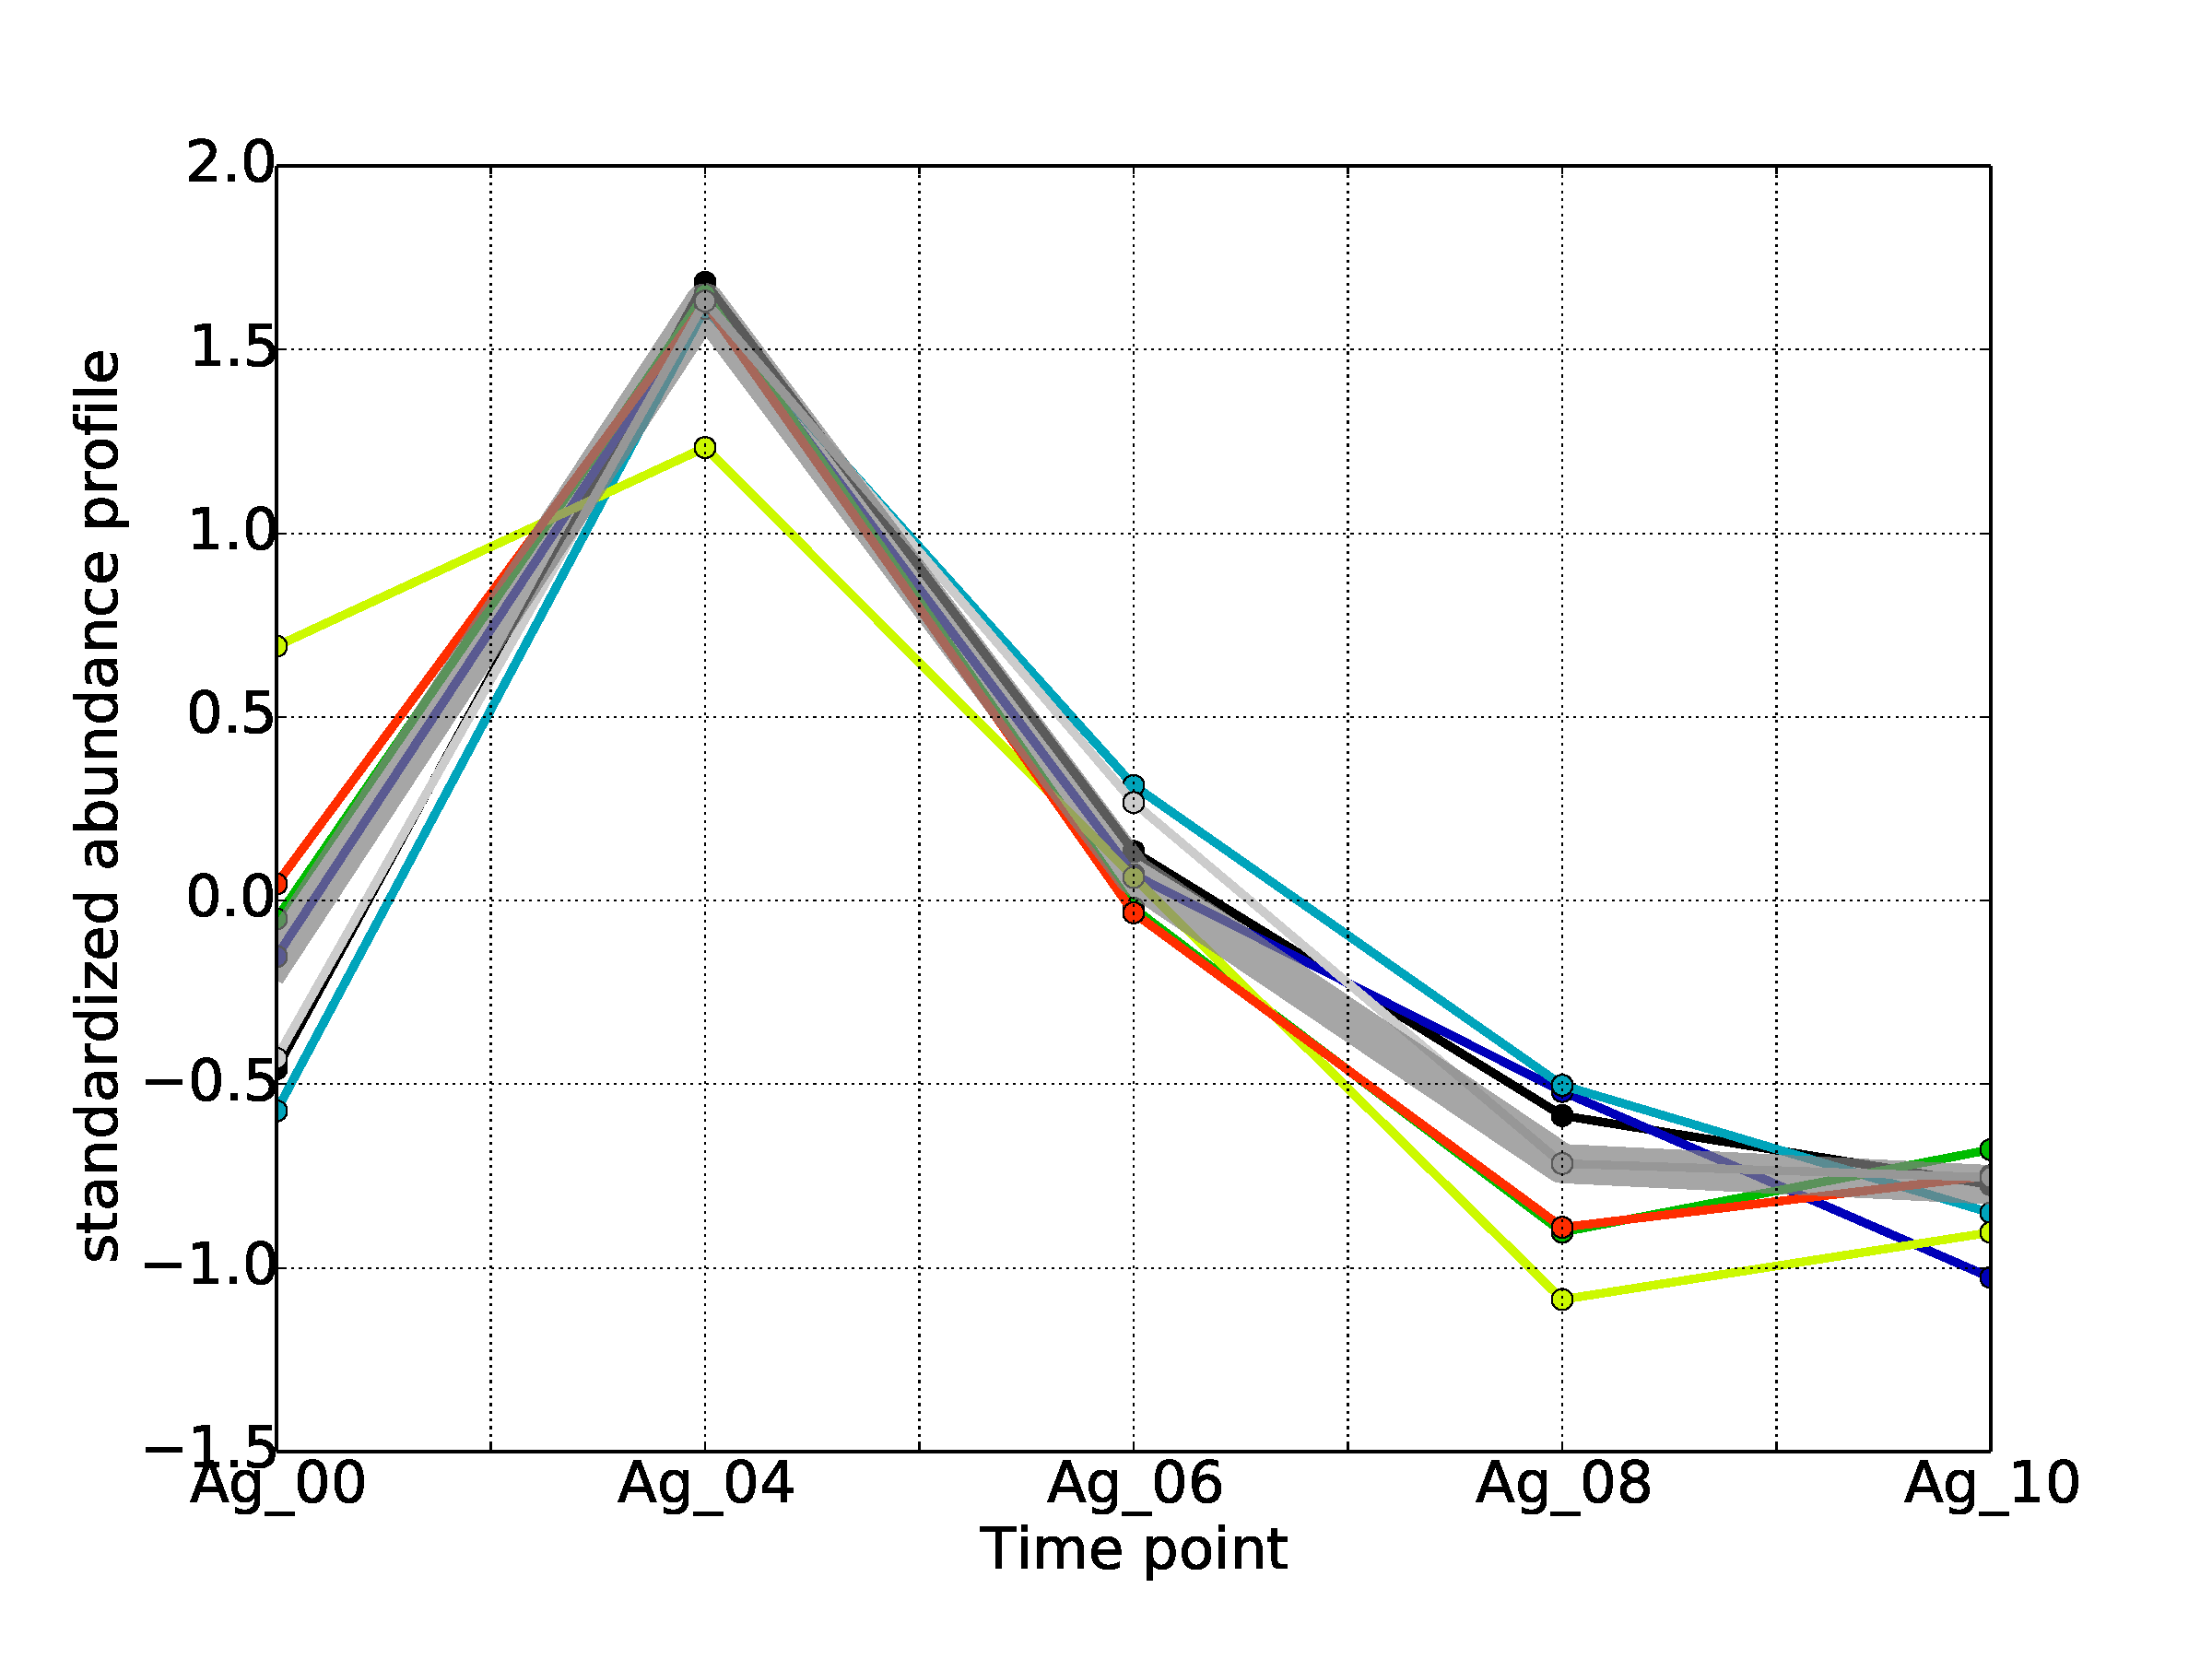
\includegraphics[width=.5\linewidth]{figures/figs/ecr_and_insects_ptci_20130918_orthodb7/upAt4_gene_profiles_from_cummerbund/Ag_upAt4_cls22_Ag_target_FPKMs_vb_orthos.pdf}}
%
\subcaptionbox{\label{fig:cluster22-Cq}}
{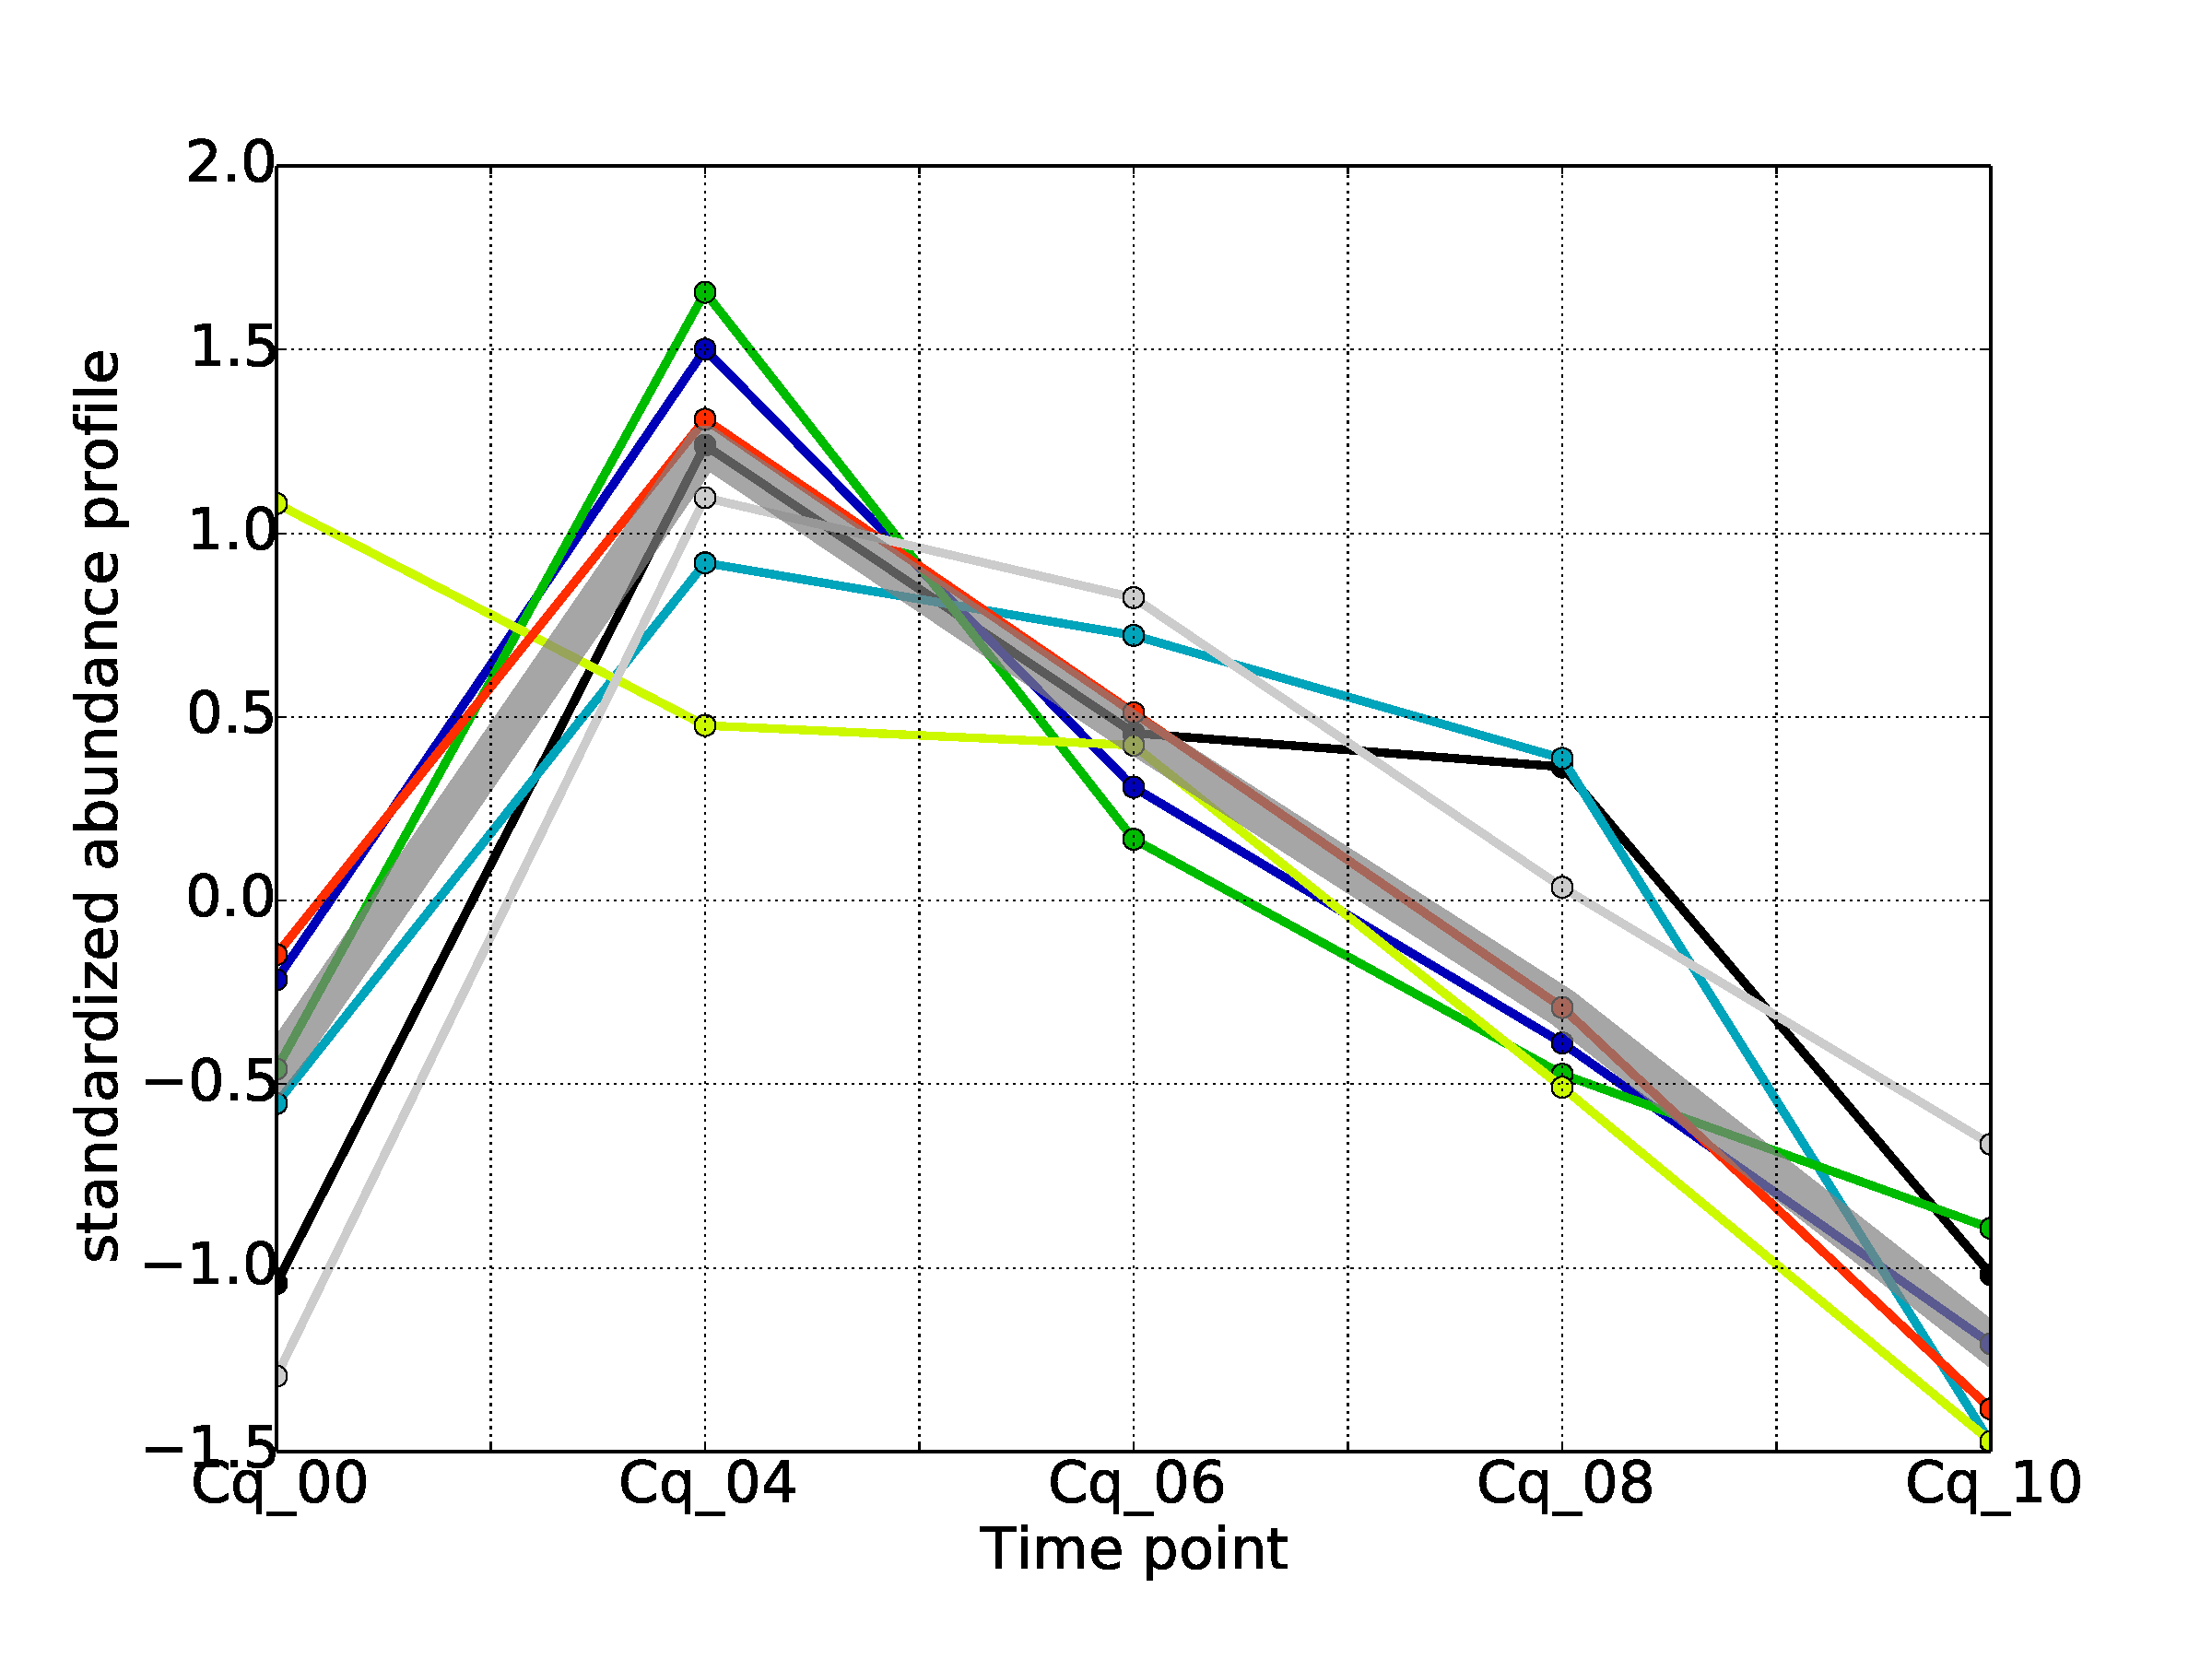
\includegraphics[width=.5\linewidth]{figures/figs/ecr_and_insects_ptci_20130918_orthodb7/upAt4_gene_profiles_from_cummerbund/Cq_upAt4_cls22_Ag_target_FPKMs_vb_orthos.pdf}}
% 
\caption[Orthologs of cluster 22]{\sf \textbf{Orthologs of cluster 22 (up at 4h):}\\
The same color scheme is used for each species which means that orthologs are given the same color in all three panels.
The thick, transparent gray line represents the median \gls{mAP} for the panel.
\textbf{(A)} \Aa.
\textbf{(B)} \Ag.
\textbf{(C)} \Cq.
}\label{fig:cluster22}
\end{figure}


\paragraph*{Functional annotations of cluster 22:}

% protein folding / translation
% membrane transport
% chromatin reoganization / link to 20E signaling pathway

% ## not found in func annotation mean tables ## AAEL011240	 AGAP006534	 CPIJ002990  --> ortholog to Dmel putzig (ptz)  annotated as described with: positive regulation of Notch signaling pathway; negative regulation of JAK-STAT cascade; chromosome organization; ecdysone receptor-mediated signaling pathway; cell cycle; neurogenesis; chromatin organization.


% transcription factors
%	AAEL011240, AGAP006534, CPIJ002990 {ortholog to Dmel putzig (ptz)}
%	AAEL002795, AGAP003943, CPIJ004011 {Rfx transcription factor}


Cluster 2 has the fewest members of ortholog-sets of the four clusters described here (7 members per species).
%
The putative functions in this cluster can be associated with protein translation and protein folding and transcription regulation and chromatin reorganization (Tables \ref{tab:cls22-process} and \ref{tab:cls22-function}).
%
Terms associated with protein translation and folding include translation initiation factor activity (20221.31), unfolded protein binding (7160.14), lysyl-tRNA aminoacylation (5305.2), regulation of translational initiation (5198.1), protein folding (5145.4), translation (3885.2), tRNA aminoacylation for protein translation (3277.1), translational initiation (3268.5), cellular protein metabolic process (2591.6), formation of translation preinitiation complex (1607.7), and tRNA processing (223.64).

% Booktabs require to add \usepackage{booktabs} to your document preamble
\begin{table}[hp]
\begin{center} \sf
\begin{tabular}{p{.7\textwidth}r}
\toprule
\textbf{Name}                                  & \textbf{Total Score (mean)} \\ \midrule
lysyl-tRNA aminoacylation                      & 5305.29                     \\
regulation of translational initiation         & 5198.13                     \\
protein folding                                & 5145.48                     \\
translation                                    & 3885.25                     \\
tRNA aminoacylation for protein translation    & 3277.15                     \\
translational initiation                       & 3268.53                     \\
cellular protein metabolic process             & 2591.65                     \\
regulation of transcription, DNA-dependent     & 2500.50                     \\
transmembrane transport                        & 2120.54                     \\
formation of translation preinitiation complex & 1607.78                     \\
transcription, DNA-dependent                   & 1314.06                     \\
signal transduction                            & 853.12                      \\
regulation of insulin secretion                & 709.97                      \\
negative regulation of BMP signaling pathway   & 526.20                      \\
regulation of cell cycle                       & 470.82                      \\
melanocyte differentiation                     & 316.77                      \\
endocrine pancreas development                 & 296.05                      \\
transport                                      & 288.59                      \\
developmental pigmentation                     & 287.51                      \\
pigmentation                                   & 273.58                      \\
tRNA processing                                & 223.64                      \\
multicellular organismal development           & 203.63                      \\ \bottomrule
\end{tabular}
\end{center}

\caption[Cluster 22 top process GO terms]{\sf \textbf{Cluster 22 top process GO terms}}
\label{tab:cls22-process}
\end{table}
% Booktabs require to add \usepackage{booktabs} to your document preamble
\begin{table}[hp]
\begin{center} \sf
\begin{tabular}{p{.7\textwidth}r}
\toprule
\textbf{Name}                               & \textbf{Total Score (mean)} \\ \midrule
translation initiation factor activity      & 20221.31                    \\
unfolded protein binding                    & 7160.14                     \\
DNA binding                                 & 4535.66                     \\
arsenite transmembrane transporter activity & 1600.53                     \\
lysine-tRNA ligase activity                 & 1557.61                     \\
cytoskeletal adaptor activity               & 1456.65                     \\
ATP binding                                 & 1146.99                     \\
aminoacyl-tRNA ligase activity              & 682.47                      \\
nucleotide binding                          & 669.32                      \\
ligase activity                             & 526.89                      \\
transporter activity                        & 400.96                      \\
zinc ion binding                            & 257.13                      \\ \bottomrule                     
\end{tabular}
\end{center}

\caption[Cluster 22 (up at 4h) mean function GO terms]{\sf \textbf{Cluster 22 (up at 4h) mean function GO terms}}
\label{tab:cls22-function}
\end{table}

Two ortholog-sets are annotated as transcription factors (AAEL011240, AGAP006534, CPIJ002990: orthologs to \Dm\ putzig; and AAEL002795, AGAP003943, CPIJ004011: Rfx transcription factors).
%
FlyBase has annotated putzig with the following terms in \Dm\, positive regulation of Notch signaling pathway; negative regulation of JAK-STAT cascade; chromosome organization; ecdysone receptor-mediated signaling pathway; cell cycle; neurogenesis; chromatin organization \cite{Marygold2013}.
%
The Rfx transcription factors were assigned regulation of insulin secretion (709.97) and endocrine pancreas development (296.05) by \gls{Argot2}.
%
OrthoDB corroborates these annotations, but only when vertebrate genomes are included in the data-set.

Membrane transport and signaling terms are also present.
%
They are arsenite transmembrane transporter activity (1600.53), transporter activity (400.96), transmembrane transport (2120.5), signal transduction (853.12), negative regulation of BMP signaling pathway (526.20), regulation of cell cycle (470.82), and transport (288.59).








\section{Discussion} \label{chap:4-sec:discussion}

% interpretation of Argot2 results (insulin/pancreas dev came from vertebrate matches and require a degree of interpretation)

% \subsection{Bloodfeeding and the midgut}

% \subsection{Heme biosynthetic process}

%%% Local Variables: ***
%%% mode: latex ***
%%% TeX-master: "thesis.tex" ***
%%% End: ***
